%todo capitalize first letters
\documentclass[12pt]{report}

% my setup file
\usepackage{thesisSetup}

\DeclareUnicodeCharacter{2060}{\nolinebreak}

\title{
    {Effect of organic fertilization on long and short term dynamics of various SOM pools and related soil features}\\ 
    {\large Institution name}\\
   % {\includegraphics{university_logo.jpg}}
}

\author{Braud Elan }
\date{February 2020}

\begin{document}
	\maketitle

%% this for using in the rcparams
%document text width: \printinunitsof{in}\prntlen{\textwidth}
%lengths
%\newlength{\figurewidth}
%\setlength{\figurewidth}{\linewidth*0.5}
	\chapter*{Abstract}
	    Soil Organic matter (SOM) is a key feature for soil health and fertility in both natural and managed ecosystems. In the last few decades there is an ongoing shift in paradigm regarding the nature of SOM and the conditions facilitating its formation and preservation. This emerging view stresses the dynamic nature of SOM, arguing that the potential preservation of SOM is essentially a soil ecosystem feature, rather than an inherent characteristic of the OM itself. It is now becoming more and more evident that optimal SOM management should also include the promotion of a viable soil biota, enabling the efficient processing of incoming OM fluxes.  \\
	    The use of Organic amendments as part of agricultural land management can increase SOM and is often regarded as a sustainable alternative to mineral based fertilization. Nonetheless, organic fertilization particularly when combined with otherwise conventional field crop management should also be examined with reference to more natural, undisturbed soil ecosystems. this is especially important in arid and semi arid climates where soils are often with very low in organic matter and are prone to erosion and other soil degradation phenomenons.\\
	    The current work compared soil samples of two contrasting, long term organically (Org) vs. minerally (Min) fertilized plots, from the long term plots of the Gilat organic agriculture project (GOP) and another soil sample from an adjacent unmanaged soil (Unm). This long-term experiment included treatment with the relevant amendments for 5 years and then one year without fertilization and another year were the soil was laid bare ('no input + fallow' period).\\
	    These soils were used to evaluate the effect of long-term fertilization and overall conventional field crop management, on both long-term changes in SOM pools as well as short-term dynamics of these SOM pools in response to substrate application. Additionally the effect of consecutive application of highly labile substrate on short-term carbon dynamics was examined. Particular attention was given to the effect of management history on the ecosystem efficiency of substrate-carbon use and potential stabilization in a short time frame.\\
	    Previous studies in the GOP have seen significant increases in total organic carbon as well as other important SOM pools such as microbial biomass and microbial activity, in Org plots compared with Min plots. Similar works from different locations have found comparable results and the general benefits of organic amendments for enhancing SOM stocks as well as improving aggregate  structure, are well documented. Therefore I expected to observe significant increases in SOM pools and related features for Org compared with Min. In terms of the short-term dynamics, I expected the efficiency of substrate use to be higher for Org compared with Min, owing to the enhancement of different SOM pools and related soil features such as aggregate structure. 
	    Conventional agricultural management is often reported to cause a reduction in various SOM pools and other related soil properties, when unmanaged soil is being utilized for crop production. Practices such as tillage, herbicide use and intensive chemical fertilization are well known as potential causes of soil degradation. Hence, I hypothesized that long-term conventional agricultural management would result in considerable reduction in SOM pools when compared with an unmanaged soil.\\
	    Two incubation experiments were set up. The first, A 7 days Straw/Compost incubation which included soil samples from the two fertilized long term treatments and the addition of a single application of either straw or compost at the start of the incubation, as well as a control treatment without amendment. The second incubation, a 28 days Model Root Exudate(MRE) incubation, included all three soils (Org, Min and Unm). These were amended with a MRE solution at day 0, 7 and 14. In both incubations the following SOM pools were measured: Total organic carbon (TOC), Water Extractable Organic Carbon (WEOC), Hot Water Extractable Carbohydrates (HWES), microbial CO2 respiration and Microbial Biomass Carbon (MBC). The content of Ergosterol, a bioindicator for saprophytic fungi, was also measured. The Straw/Compost incubation included also the analysis of total organic carbon in a hot water extract and the MRE incubation included an Aggregate stability test besides the above mentioned tests.  The results from the control treatment in the MRE incubation were used to calculate baseline values for each of the measured parameters, allowing the comparison of the different long term treatments in terms of their effect on the normal status of these parameters. Microbial biomass and microbial respiration data were used to calculate a Carbon Use Efficiency measure.\\
	    Total Organic Carbon (TOC) was significantly higher in Org compared with Min and likewise, baseline values  for most other SOM pools were higher in Org over Min (though differences were mostly insignificant). Interestingly, Org - and Min to a certain extent - presented significantly higher baseline values than Unm, in TOC, basal respiration, \gls{mbc}, \gls{weoc}, \gls{hwes} and \gls{ags}.\\ 
	    MRE applications resulted in a clear reduction in CUE for all three long term treatments. Likewise, the degree of labile soluble carbon (WEOC) removal from the soil system decreased substantially between consecutive MRE applications. The intensity of WEOC removal was deferentially expressed in the three LTTs with Org $  > $ Min $ > $ \gls{unc}, and these differences were very apparent. No clear differences were observed between LTTs in terms of CUE.\\
	    My results showed considerable enhancement of SOM pools after 5 years of compost application, when compared with mineral fertilization. Interestingly, this management history effect was noticeable despite the \textit{no input + fallow} period that preceded soil sampling for the current experiment, demonstrating the persistent effect of organic fertilization. The substantial increases in SOM pools and AS for Min and particularly Org, compared with \gls{unc}, were of special interest since this result is in disagreement with most \hiddenTxt{a bit to determind?} of the works on the subject. However, a number of studies have shown that in certain settings, for example such as an arid or semi-arid environment, cultivation may indeed enhance SOM pools when compared with a unmanaged soil. This was linked with the ecosystem's \gls{npp} and the fact that given the specific conditions in an arid or semi-arid climate, agriculturally managed soil can often sustain higher NPP compared with an unmanaged soil.\\
	    The differences observed between LTTs with regard to WEOC dynamics, suggest that increases in total SOM stocks, MBC and AS, as a result of long-term organic fertilization, had a substantial impact on the soil's capacity for removal of labile carbon from the dissolved fraction. Since no significant differences in CUE were noted between LTTs, it remains unknown whether this variability in WEOC removal was also related to differences in potential carbon stabilization. Nonetheless this outcome suggests increased MBC and microbial activity (as expressed in microbial respiration) and possibly an improved soil aggregate structure, can facilitate a higher decomposition capacity and increased potential for organic carbon stabilization as part of SOM.\\
	    A conceptual model was proposed, describing the key factors involved in the potential short-term stabilization\textbackslash mineralization of incoming carbon. Based on this model, substantial decreases in CUE were related to a shift in the proportion between three key features of the soil system, i.e. size of the active microbial population, the quantity of labile substrate and the frequency of soil spatial sites of potential carbon stabilization. This analysis suggested that increased substrate load unaccompanied by similar increases in sites of potential carbon stabilization can result in substantial reductions in CUE. This reiterates the importance of a developed soil structure for the efficient use of incoming organic carbon.\\
	    This study provided further support for the use of organic amendments to enhance SOM stocks and other important SOM pools. Setting the Compost treated samples against an Unmanaged soil, illustrated the variability of soil response to crop land management, and showed that cultivation, particularly when combined with organic amendments, such as composted animal manure, can improve soil fertility and health.\\
	    Furthermore, results from the MRE incubation indicated a substantial effect for management history in terms of the microbial capacity for utilization of labile carbon (WEOC) in the short-term of a few days. Although this result is confined to a very short-term and does not explicitly include CUE or other carbon stabilization indicators, it is nonetheless a valuable clue to the effect of long-term fertilization and overall management on the soil's short-term reaction to incoming substrate. This can have important implications for long-term SOM dynamics under different land management schemes.  
	    
	    
	    
	    %   continues and steady flux of labile carbonaceous substances (e.g plant root exudates)   
	    

	\chapter*{Dedication}
	    I'd like to thank this and that

	\chapter*{Declaration}
	i declare

	\chapter*{Acknowledgement}
%todo include Nadia Buchnovsky for Ergosterol work
	\tableofcontents

	\chapter{Introduction}
	% !TeX root = ../main.tex
	
		\section{Benefits of soil organic matter}
		
		
		\gls{som} is a key factor in maintaining ecological services provided by soil ecosystems.
		\gls{som} contributes to soil fertility and health by retaining plant-available water and nutrients and promoting the formation of soil structure. \gls{som} is also consumed in the process of arable soil management as it releases needed nutrients and energy when it decomposes. Indeed soil organic matter is often highly beneficial when it decays and releases energy and nutrients \citep{lehmann2015, janzen2006}. Therefore it is important to explore  management practices that will allow both the accrual and simultaneous  decomposition of organic matter in a balanced ecosystem.
		
		\section{Shift in paradigm regarding \gls{som} formation}
		
		In the last  decades, there is an ongoing shift in  paradigm, concerning the nature of \gls{som} formation and retention in the soil. This shift is from what is sometimes referred to as the ‘humification’ model, in which the persistence of \gls{som} is mostly associated with the molecular structure of organic matter, to a more ecological framework (soil continuum model) that emphasizes the importance of environmental and biological factors in controlling the turnover of organic matter \citep{lehmann2015}. in the historical, \textit{humification} model, above-ground plant carbon inputs were regarded as the main source for \gls{som} formation. Stable organic matter was seen to comprise mainly selectively preserved plant inputs and de novo synthesis products like humic substances, whose chemical complexity and composition render them nearly inert relative to microbial degradation.\\
		The emerging understanding is that the molecular structure of organic material does not necessarily determine its stability in soil. Rather, \gls{som} cycling is governed by multiple processes shaped by environmental conditions (such as physical heterogeneity)\citep{schmidt2011c}. this shift in paradigm was fueled by a number of novel discoveries regarding the nature of \gls{om} decomposition and stabilization in the soil. Firstly, the preservation of recalcitrant plant material as a basis for \gls{som} accumulation was repeatedly rebuked by evidence demonstrating the ability of soil microbes to rapidly decompose almost any biologically derived substance \citep{dungait2012, marschner2008} and the preferential stabilization (i.e longer turnover time) of labile plant products over recalcitrant materials has been demonstrated in a number of experiments \citep{cotrufo2013, kleber2011}. Concurrently, the existence of stable, large and complex molecular structures in the soil(i.e humification products) was substantially called into question\citep{kleber2010}. finally the outlining of a number of previously under-recognized mechanisms for stabilization and preservation of \gls{om} in the soil was detailed in several papers, emphasizing the role of reduced accessibility for microbial decomposition (i.e. physical protection inside aggregates and chemical bonding to mineral surfaces), as a primary determinant of \gls{om} stabilization and persistence\citep{lutzow2006, lutzow2008, ekschmitt2008}\.\\
		This new framework for \gls{som} formation stresses the dynamic nature of \gls{som} management, wherein the preservation and enhancement of \gls{om} in a living soil (such as topsoil) depends not on the minimization of decomposition activity, for example by providing recalcitrant \gls{om} amendments or by targeting \gls{om} supply into areas of lower microbial activity (such as subsoil), but rather on the continuous supply of labile organic inputs, inducing high levels of microbial activity, which is able to facilitate the efficient formation of organo-mineral bonds and the protection of \gls{om} within aggregates\citep{dungait2012,barre2016,basler2015}.
		
		
		\section{Microbial population as an essential component in \gls{om} cycling}
		
		The soil microbial population is the major biological compartment responsible for decomposition and transformation of organic inputs \citep{thiet2006}. A growing body of evidence demonstrates that microbial products are the largest contributor to stable \gls{som} and that \gls{som} formation rates are positively and closely connected with the growth rates of microbial biomass \citep{kallenbach2016, kallenbach2015, ludwig2015, schurig2013, bradford2013}. Microbes drive \gls{som} formation through several mechanisms, both direct and indirect. Cell components of dead microbes are now considered a major source for stabilized \gls{om} \citep{kallenbach2015, liang2011, miltner2009} and it has been shown that these microbial remains are often preferentially concentrated in the more stable fractions of the soil \citep{ludwig2015}. \citet{liang2011} estimated that microbialy derived substances could make up more than 80\% of \gls{som}⁠.
		%  	the soil amino acid signature has been found to correlate  with the  bacterial community structure
		%  	\citep{moon2016}.
		\citet{kiem2003} found polysaccharides, mainly those of microbial origin, are stabilized over the long-term within fine separates of arable soils.\\
		Apart from being a major source of readily stabilized \gls{om}, micro-organisms are highly involved in the  modification of the soil environment, providing conditions that enhance the further decomposition and stabilization of additional \gls{om}.  For example, the production of extracellular substances by some micro-organisms is strongly related to the formation of aggregate structure and the mediation of water and oxygen concentrations, thus creating favorable growth environment and allowing for increased capacity for organic matter stabilization \citep{schimel2012} ⁠and as already mentioned, microbial remains form a large fraction of stabilized \gls{som} and have an important role in the formation of stable aggregates. Similarly, the release of organic acids by certain microbes has been shown to promote \gls{som} formation through increased mineral dissolution and mineral availability, thus increasing the potential for organo-mineral bonding \citep{yu2018}.
		
		
		
		\section{Substrate Use Efficiency }
		%todo force \gls{cue} to present long form 
		%todo find a better term for 'neasure' in 'This \myRed{measure} a common indicator for overall substrate...'
		Microbes metabolize a wide variety of compounds to satisfy demands for \gls{carbon} and energy, thereby influencing the accumulation/loss dynamics of soil organic matter stocks and ecosystem carbon dioxide efflux \citep{xu2017}. The efficiency with which microorganisms convert available organic substrates into stable, biosynthesized products is a critical step in ecosystem \gls{om} cycling. \gls{cue} is defined as the ratio between the amount of substrate-C incorporated into microbial biomass and the amount of substrate-C consumed. This \myRed{measure} a common indicator for overall substrate use efficiency of the soil. The relevance of microbial efficiency spans scales ranging from a single microbial cell to entire ecosystems and variation in \gls{cue} has been linked to substrate biochemistry, thermodynamic and genetic capacity of the cell and microbial community structure and activity\citep{kallenbach2019, soares2019}. Other approaches have explored \gls{cue} from the ecosystem perspective, studying the effects of altered efficiency on the mediation of ecosystem services such as C sequestration. A considerable number of different experimental settings, methods and definitions have been used for the evaluation of \gls{cue} over the years, depending on the discipline and ecological framework in which \gls{cue} was examined. \citet{geyer2016} suggested a classification of \gls{cue} based on the ecological and temporal factors associated with the different definitions of \gls{cue}. The ecosystem perspective of carbon use efficiency (\gls{cue}$ _E $) as defined by \citet{geyer2016}, integrates drivers originating from population and community scales, as well as time-dependent factors such as biomass turnover and the recycling of necromass and exudates that occur external to the cell. Due to the relatively longer time periods associated with it (days to weeks), \gls{cue}$ _E $ reflects, on top of microbial community factors, environmental variables such as soil mineralogy, surface area and in fact any environmental factor that may exert influence on the turnover of microbial biomass and recycling of organic substrates. In this work, \gls{cue} will mostly be considered in the ecosystem context corresponding to \gls{cue}$ _E $.\\
		The drivers for efficient decomposition and cycling of organic carbon, in an ecosystem context, are evidently complex.
		Soil features such as mineralogy and aggregate structure may have a significant effect on \gls{cue}, particularly when microbial turnover and recycling of organic substrates are considered. For example, \citet{kravchenko2019} found the abundance of soil pores of size category 30 - 150 $ \mu m $ to be pivotal for the efficient stabilization of carbon through microbial activity. These pores act as sites for enhanced microbial activity and processing of new C input as they provide optimal water and oxygen supply. High abundance of such pores was found to ensure a large proportion of the soil matrix in close proximity to active microbial communities. In this way, microbial decomposition products and necromass have a greater chance of being stabilized in the soil through interaction with mineral surfaces and physical protection within soil aggregates, rather than being lost by mineralization.
		\citet{tian2015}, examined the effect of aggregate disruption on glucose decomposition and found significantly lower \gls{cue} for crushed, compared with intact macroaggregates. They concluded that aggregate structure must have an important role in shaping the dynamics of microbial decomposition of input C.
		
		\section{Stabilization of \gls{som} closely connected with aggregate formation}
		
		The above mentioned works, along with a  number of other recent studies have made it evident that soil aggregation and the spatial organization resulting thereof, are central elements determining the fate of new input C. At the same time, the stabilization and incorporation of organic materials as part of \gls{som}, serve as a primary mechanism in the processes of aggregate formation. As noted earlier, newly recognized mechanisms of \gls{som} formation and preservation, include the physical and chemical protection of \gls{om} within and as a part of soil aggregates. Physical protection entails the inaccessibility of certain soil pores to micro-organisms and exoenzymes, making them optimal sites for the preservation of \gls{om}. This can result for example from actual size restrictions or the occurrence of conditions such as low oxygen availability which may preclude microbial utilization of \gls{om}. Chemical protection involves an array of organo-mineral interactions that can render \gls{om} inaccessible for microbial decomposition. By being chemically bonded to mineral surfaces, organic substances aid the formation of soil aggregates, acting as a gluing agent, rearranging soil particles into micro and macro aggregates \citep{six2002}. Thus, incoming \gls{om} (from plant origin or amendment source) acts as both the source of \gls{som} stocks and a major drive in the formation of soil structure, providing the platform for further stabilization and preservation of new incoming \gls{om} \citep{mccarthy2008}.\\
		While aggregate structure can enhance the stabilization of \gls{som}, the biological contributions to aggregate formation and stability are dependent on a supply and turnover of \gls{som} by micro-organisms. If the supply of \gls{om} is restricted, the aggregate stability declines and \gls{som} persistence is diminished. Therefore, the maintenance of stable aggregates  depends to a large extent on the turnover of \gls{som} in aggregates to sustain soil microorganisms \citep{dungait2012, golchin1994}.
		
		%todo rephrase this?
		\section{Labile organic matter}
		
		Labile, light weight organic substrates are increasingly recognized as having a major role in the formation of stable \gls{som}.
		Root derived inputs and specifically root exudates, constitute a significant source of such readily available organic carbon substrates.  It is assumed that about 20\% of all $ CO_2 $ assimilated in crop plants is deposited by roots into the soil as labile substances, generally referred to as rhizodeposits, and this percentage can be as much as 30-40\% in perennial grasses and other perennial plants \citep{kuzyakov2004, pausch2013, pausch2018}. Root derived carbon is much more likely to be incorporated into the more stable fractions of \gls{som} than above ground plant residues \citep{austin2017, kong2010, puget2001, rasse2005}.\\
		Rhizodeposition vary extensively in both composition and output rate according to plant species, physiological state and environmental conditions \citep{dennis2010, pausch2018, jones2004}. Furthermore, although it has a fundamental role for organic matter dynamics in the soil, it’s quantification under field conditions remains limited \citep{pausch2018}. Estimations of the rate of exudation for Maize plants for example, can vary extensively\citep{nguyen2003, pausch2018}.
		
		\section{Dissolved Organic Matter}
		
		\citet{zsolnay2003} proposed the generic use of the term \gls{dom} when referring specifically to the organic matter truly dissolved in situ. Other soil solutions obtained through extraction with batch or percolation methods, such as the \gls{weom} or \gls{hweom} represent the \textit{potentially} soluble organic matter \citep{marschner2003}. DOM is a complex mixture of different components that can vary widely in both its composition and concentration depending on soil conditions  as well as on the method of extraction\citep{bolan2011}. DOM is often  correlated with \gls{som} stocks and indeed a number of relatively recent studies have shown \gls{som} to be the prime source of DOM as opposed to  recent plant derived \gls{om} \citep{malik2013, kaiser2012}. \citet{malik2013}showed that  even after a very high plant biomass input, plant-derived carbon in DOC was less than 40\%.\\
		The mechanisms and controls over \gls{som} decomposition processes, including solubilization  into the DOM pool are numerous, with both biotic and abiotic factors playing a significant role\citep{kalbitz2000, bolan2011}. Studies have shown that the microbial population is highly involved in the production and consumption of DOM \citep{marschnerp2002, malik2013, guggenberger1998}.  DOM has been characterized as being in a dynamic equilibrium with the solid phase \gls{som} \citep{roth2019, kaiser2012},  with the transfer of microbially processed organic molecules back and forth between solid and soluble phases controlled to varying degrees by  direct (exoenzymes) \citep{guggenberger1998},  and indirect(removal of solublized \gls{om} thus increasing diffusion gradient) solubilization of mineral associated \gls{om} as well as by microbial processing of recent ( mostly plant source) \gls{om}, making it more available for interaction with mineral surfaces \citep{kalbitz2003, kalbitz2008}.These features of the DOM pool position it as an intermediate \gls{om} pool, through which \gls{som} is made available to microbial consumption. Thus, DOM can provide valuable clues for microbialy mediated \gls{som} processes. \\
		
		\section{Hot Water Extractable Carbon and Hot water extractable carbohydrates}
		
		\gls{hwec} represents a pool of potentially dissolved \gls{om}, less available than WEOC yet of a more biodegradable and labile nature \citep{chantigny2014, leinweber1995, gregorich2003}. HWEC is regarded as being weakly bonded to mineral surfaces or physically protected within soil aggregates and is a source for microbial consumption \citep{zakharova2015, leinweber1995}.
		HWEC is considered a  sensitive indicator of changes in soil management and \gls{som} dynamics, often responding to changes much faster than total organic carbon measures \citep{ghani2003}. HWEC is correlated with a number of important biochemical soil properties, among them, \gls{toc}, MBC and aggregate stability \citep{hamkalo2014}.
		a considerable fraction of HWEC is composed of Carbohydrates \citep{leinweber1995, balaria2009}. \citet{ghani2003} found between 40-50\% of HWEC was in the form of carbohydrates in a series of grassland soils.
		\gls{hwes} where found to  closely reflect changes in aggregate stability \citep{haynes2005, yousefi2008, leguillou2012} and it is suggested that they have a major role as binding agents in the formation of soil aggregates.
		HWES are considered to be mostly of microbial origin \citep{haynes1993, debosz2002}, yet the proportion of unprocessed plant derived constituents can vary, depending, at least to a certain extent, on the level of microbial activity and the stability of the soil fraction from which carbohydrates are extracted. \citet{puget1998}, \citet{jolivet2006} and \citet{bock2007} all found microbially derived carbohydrates to be preferentially bonded to the most stable soil size fraction (caly + silt), indicating both the importance of certain  carbohydrates in stable aggregate formation and the fact these carbohydrates are mostly of microbial origin.
		Considering its close relation with aggregate formation and microbial growth and production, it is plausible that HWEC act as a substantial factor in  the dynamics of \gls{som} stabilization, at least for short term processes.
		
		\section{Effect of management history on the long term dynamics of \gls{som} properties}
		
		\subsection{Fertilizers and \gls{om} amendments}
		
		The application of organic and inorganic amendments is a common practice in agricultural soil management. Long-term application of organic amendments, exclusively or in combination with mineral fertilizers, has been shown to increase TOC \citep{heinze2010, yang2012} as well as MBC \citep{luo2015, marschner2003a}and aggregate stability\citep{ huang2010, yu2012} compared with an non-amended or mineral-only fertilized soil.
		studies examining the effect of long term organic-only compared with mineral-only fertilization had  also shown clear evidence of a beneficial effect of organic fertilization on TOC\citep{santos2012, luo2015}, while the effects on more sensitive parameters such as MBC, HWEC and AS are sometimes less consistent \citep{albiach2001, mahmood1997}. It should be noted that results for this kind of comparison often depend on the choice of organic or mineral amendment as well as other management factors.    
		For example, Liu et al. (2013) found  higher MBC in long term manure compared with Urea-N fertilized soil, while no significant difference in MBC was observed when a Phosphorus fertilizer was added to the Urea-N treatment. Additionally they estimated the annual total carbon input from crops as well as amendment carbon and these estimates had shown a ~35\% more input carbon in the manure treatment compared with the N-only treatment, not including the carbon input from manure amendment itself (i.e, in-field plant derived carbon). This hints at the importance  of plant productivity enhanced by organic or inorganic amendments, in determining the  effect of fertilization on soil biochemical parameters.\\
		Besides management effects, \gls{som}  related parameters may also be subject to high seasonal variability in agricultural systems, depending on environmental changes as well as management interventions, further complicating the definite identification of long term fertilization effects\myRed{*}.
		Diallo-Diagne et al. (2016) found higher MBC in manure fertilized soil compared with Urea-N fertilized soil in the beginning of the growing season, yet these differences faded at flowering stage and at harvest. Other works have also found significant temporal variations in MBC between years \citep{kaiser1995} and plant physiological state \citep{jat2020}\\
		It is evident therefore, that the effects of organic compared with mineral fertilization management in agricultural systems, with regard to the accumulation of SOC or the enhancement of other \gls{som} pools such as MBC, WEOC and HWEC, are not entirely clear.
		
		\subsection{Effect of arable land management on \gls{som} properties}
		%todo find more references for adverse effect of nitrogen fertilization, especialy with regard to reduced rehizodeposits or reduced carbon stabilization...
		Arable land management, and particularly intensive, modern day agricultural crop management practices, are well recognized as a serious environmental concern, along with its obvious contribution to human economy and well being.
		Modern agricultural is at the same time an invaluable resource for the earth’s population and a growing concern among researchers and environmentalists for the numerous adverse effects it entails, such as, pollution and eutrophication of natural water bodies \citep{liu2012,rabalais2002}, greenhouse gas emissions\citep{vermeulen2012}, loss of biodiversity\citep{laurance2014} and soil degradation\citep{grunwald2011}.
		Because of these two contrasting effects of agricultural intensification, it is important to continuously evaluate the benefits of different agricultural management schemes with reference to more extensive agroecosystmes as well entirely non-cultivated land which are often not as susceptible to soil degradation/environmental damage.
		Natural, non-cultivated soils are usually characterized by minimal physical disturbance, little or no chemical inputs and an all year round soil cover (either live plants or dried stalks of annual plants), while arable soils are mostly subject to higher degrees of physical and chemical soil disturbance.
		these characteristics of cultivated and non-cultivated soils are general, and clearly large variability can be expected within these broadly defined features. For example, differences in vegetation type and plant coverage are evidently expected for non-cultivated soils, depending on the specific climatic and environmental conditions prevailing. for agriculturally managed soils, variability may be much higher considering the wide range of practices common in arable land management.
		A large body of evidence suggests that land conversion of undisturbed, non-cultivated soils into arable soils can cause significant reductions in \gls{som} stocks \citep{ashagrie2007, spaccini2001, ogle2005}.
		native land conversion has also been shown to cause reductions in aggregate stability \citep{bongiovanni2006, cambardella1993,  elliott1986}, nad microbial biomass \citep{mganga2016, soleimani2019} and diversity\citep{monkai2018}.
		the underlying drivers for these reduction in \gls{som} and related properties, through native land conversion, can be numerous and complex. Tillage, fertilization, reductions in plant cover, annuality vs. perenniality and loss of biological diversity are some of the major factors that can adversely affect \gls{som} properties.
		Tillage is a common agricultural practice, often considered a major driver for soil degradation where native soils are shifted towards agricultural use (Murty 2002; Six 2002). The negative effect of tillage on \gls{soc} as well as aggregate structure is often observed in experiments comparing no-till or reduced tillage treatments with conventional tillage practices \citep{six1998, west2002}.
		Differences in tillage practice have  been shown to affect the MB of the soil \citep{jat2020, alvaro-fuentes2009, sun2011} as well as
		microbial community features such as composition, activity and functional diversity, with possible consequences for the dynamics of \gls{som} \citep{vangroenigen2010, govaerts2007}. These evidences prove the marked effect that physical disruption can have on soil biology and the processes of carbon retention and preservation. This is clearly demonstrated in the work of \citet{plaza2013}, in which significantly higher levels of mineral-associated carbon were observed in a long-term no-till treatment compared with conventional tillage treatment.\\
		Introduction of inorganic forms of Nitrogen as well as other inorganic elements, is another agricultural practice that can have adverse consequences for cultivated soils compared with non-cultivated soils.  \citet{khan2007} had  presented extensive evidence demonstrating a net reduction in SOC as a result of long term nitrogen fertilization despite substantial increases in C return to the soil. \citet{egerton-warburton2000} found significant reductions in \gls{amf}  species richness, diversity, spore abundance and root colonization as a result of inorganic nitrogen pollution in a series of native scrubland soils in southern California. Numerous other studies have shown the adverse effect of mineral nitrogen fertilization on AMF diversity and abundance in agricultural settings \citep{bradley2006,treseder2004,zhang2019,corkidi2002}.  AMF are regarded as key players in the transfer and allocation of rhizodeposits, and are strongly associated with soil aggregation through fungal hyphe and the production of extracellular substances \citep{rillig2006,leifheit2014,rillig2002}. It is evident therefore that synthetic nitrogen fertilization can strongly affect soil carbon and aggregate dynamics, through the restriction of AMF activity.\\
		Despite these well documented adverse effects of cultivation practices on \gls{som} properties, significant variation may exist in the response of soil to agricultural intensification, depending on climate factors such as precipitation and temperature. For example, a meta-analysis by Ogle et al (2005), found long-term cultivation had caused the greatest loss of SOC in tropical moist climates and lowest loss in temperate dry climate, demonstrating the variable nature of soil response to long-term cultivation in different climates.\\
		
		\section{Effect of management history on short-term dynamics of \gls{som} properties}
		
		Apart from having a strong impact on SOC stocks as well on other \gls{som} related properties, management history can also have consequences for short-term dynamics of biochemical properties, when organic substrates are introduced into the soil, either as amendments or through plant deposition. Specifically, land use and fertilization management can affect the efficiency with which new organic inputs are decomposed and further stabilized as \gls{som} \citep{lee2014}. \gls{cue} has been shown to reflect long-term changes in soil management  while the underling mechanisms responsible for these variations in \gls{cue} are not entirely clear \citep{kallenbach2019}.
		\citep{kallenbach2015} applied the concept of \gls{cue} to try and explain higher long-term SOC accumulation in organically compared with conventionally managed soil, despite direct annual carbon inputs being slightly higher in the conventionally managed soil. Their findings demonstrated significantly higher \gls{cue} in the organically managed soil and it was suggested that this higher \gls{cue} combined with higher microbial growth rates, resulting in higher microbial biomass and subsequently higher necromass, was a key factor in resolving the seemingly paradoxical phenomenon of increased SOC despite similar or even lower annual carbon inputs. Differences in \gls{cue} were mainly attributed to the inclusion of a leguminous cover crop in the organic management cropping cycle, which increased the chemical diversity of available organic matter and provided high quality (low C:N ratio), energy rich substrate, in this way favoring higher community-level \gls{cue}.
		\citet{roller2015} suggested that changing resource availability, caused by management, can cause a shift in microbial community composition, affecting \gls{cue}. Increased organic carbon availability, resulting in increased \gls{cue}, have been similarly suggested by other authors \citep{cotrufo2013}.
		Increased chemical as well as spatial heterogeneity of the soil environment may select for more efficient microbial communities \citep{pfeiffer2001, nunan2017}. Chemical heterogeneity could be achieved by diversification of organic inputs. Organic amendments, such as composted manure can provide a large number of different organic substances \citep{zbytniewski2005} and in this way greatly increase the  variety of substrates that the microbial population is exposed to. This could mean higher \gls{cue} for organically fertilized soils compared with mineral-only fertilized soil.
		As mentioned earlier, soil aggregation and the spatial arrangement of soil pores are major sources of heterogeneity and have been identified as important drivers of microbial efficiency\citep{kravchenko2019}.
		Tillage reduction or elimination can induce significant changes in aggregate stability and soil structural features \citep{alvaro-fuentes2009, barreto2009} and thus affect microbial efficiency.
		although much work has been done to expose the drivers and mechanisms that control microbial \gls{cue}, a lot of this work has concentrated on the short term effects of substrate quality and availability, microbial species physiology and community dynamics. less attention has been given to the effect of long term management decisions such as fertilization and the overall effect of land use on this essential component in \gls{som} cycling. Thus the nature and underlying drivers of these effects are still not clear.
		
		\section{Short-to-medium term dynamics of organic substrate decomposition as essential components in understanding long term \gls{som} dynamics}
		
		Microbial efficiency is obviously affected by a large number of biological and environmental factors and temporal considerations are important in defining the scope of factors expressed in microbial efficiency measures such as \gls{cue} \citep{kallenbach2019}. Incubation experiments, studying the decomposition of labile organic substrates, in the time range of days to months,  can demonstrate the effects on \gls{cue} of both physiological microbial population traits (usually associated with short-term periods of a few hours to a couple of days) as well as microbial community interactions with environmental factors such as soil physical and chemical features (usually more common in the days to months range) \citep{geyer2016, manzoni2018}. Moreover, medium term experiments are also important for the fact they can provide insight into the primary stages of labile substrate decomposition in the soil, as these processes are often mostly confined to these time ranges(days to weeks) \citep{blagodatskaya2011, schneckenberger2008, tian2015}. Although \gls{som} accumulation as well as other associated processes such as the development of complex aggregate formations, often require long time periods to materialize, especially in intensive agroecosystems \citep{grandy2007}, this gradual transformation is driven by short-term instances of organic matter decomposition and stabilization \citep{kuzyakov2015}. This is particularly valid for situations in which growing plants and especially plant root deposition are the major sources of organic inputs. Root deposition and labile organic substances in general, are often significant sources of readily stabilized organic matter, and it is therefore important to consider their short to medium term decomposition dynamics with regard to long term trends in \gls{som} stocks.
		
		\section{Research objectives}
		
		The main objective of this research was to examine the effects of long term, opposing management treatments, organic compared with mineral fertilization, on \gls{som} pools,  with reference to a non-cultivated soil. This is of particular importance in arid and semi arid climates, where the effect of agricultural intensification on \gls{som} properties may not be as straightforward as is often the case for soils in other climate zones.
		This main objective was split into two specific objectives, studying the effect of management history from two aspects:
		\begin{enumerate}
			\item \textbf{Effect on \gls{som} pools in non-amended samples.} for this purpose, the dynamics of non-amended samples was closely monitored in a set of two, short-term incubations, accounting for the normal fluctuations in \gls{som} properties and thus providing reliable indication of long term management effect.
			\item \textbf{Effect on the short-term dynamics of \gls{som} pools in reaction to labile organic input.} the short-term effect of labile organic amendment was examined in the different long-term treated soil samples, assessing any possible differences between these soil samples, upon specific sampling events as well as with regard to the overall trends.
			
			\numintertext{Additionally, a secondary objective was put forth:}
			
			\item \textbf{Examine the effect of successive labile organic substrate applications on the short dynamics of SOM properties.} In accordance, three portions of labile substrate, applied within a two week period, were designed in  order to help identify possible mechanisms involved in short term carbon stabilization and carbon loss, as it is implied by our earlier discussion that the interaction between substrate load and other soil components (mainly microbial population and soil
			\pdfmarkupcomment[markup=Highlight, color=yellow]{physical characteristics}{indeed we dont have soils with a range of physical features. However we dont really have a range of soils for any other feature (only three soils). the reason I put in 'physical properties' is because we measured Aggregate stability and I discussed this property extensively in the discussion and particularly in the section dealing with the effect of consecutive MRE applications.I thought there should be some mention of here.}
			) may have a substantial impact on short term carbon dynamics .
		\end{enumerate}
		In exploring these objectives, particular consideration was given to microbial biomass size (MBC)  and activity (CO2 respiration) as they were assumed to express the essential role of microbial populations in SOM dynamics. Similarly, DOM dynamics, reflected in cold and hot water extractable \gls{om}, were given a significant focus as they are known to correlate with microbial features, especially those related to the active microbial biomass.  Considerable attention was also given to the aggregate stability parameter as an important indicator of soil structural features and to the HWES, representing microbialy produced stable SOM precursors, as well as important bonding elements in the formation of soil aggregates.
		%todo add sentence about the use of Ergosterol analysis and its purpose.
		
		\section{Research hypothesis}
		%todo what is 'those described previously' in the end of the following paragraph?
		Considering the well recognized adverse effects of fertilization, tillage and other agricultural practices, I hypothesized that the lack of agricultural management in non-cultivated plots will have increased SOM stocks and other related properties, compared with the cultivated soil plots. I assumed that the elimination of tillage and other physical and chemical disruptions associated with cropland management, would have warded off SOM depletion, often observed for tilled soils, while inducing increased aggregate formation and biological activity (MBC, basal respiration)  compared with the cultivated soils through the extended presence of vegetative ground cover and increased above-ground diversity . These factors were also speculated to have a positive effect on \gls{cue} and the short term decomposition dynamics of recent organic input.\\
		Comparing the long term organically with the minerally fertilized soils, I expected to observe higher SOM stocks as a result of long-term application of organic fertilizer, due to increased carbon input from fertilizer as well as increased aggregate formation that could have further enhanced the stabilization of input carbon.  I also expected increased microbial efficiency in processing recent organic substrate in the organically fertilized soil, mainly due to a more developed aggregate structure but also through increased chemical heterogeneity and possible long term effects of substrate availability causing shifts in microbial community composition.
		as for the effect of sequential labile carbon additions I expected consecutive applications to result in reduced microbial efficiency and would consequently lead to reduced levels of HWEsugars and AS.  I hypothesized that the close proximity of three high rate labile organic input applications would produce conditions similar to those described previously, resulting in reduced microbial efficiency.
	

	\chapter{Materials and Methods}
		% !TeX root = ../main.tex
		
		% questions for asher
		% 1. KWC, what is a better term for that?
		% 2.
		
		%todo include a section about modeling of respiration dynamics
		
		\section{Soil sampling}
		The soils for this experiment were sampled from the long term plots installed at Gilat in 2009 as part of the organic agriculture project (\gls{gop}), Bar-Tal et al (2017). The Gilat Research center is situated in the northern Negev(31$^\circ$20' N, 34$^\circ$41' E), the climate is a semi-desert (average precipitation $ 237_{mm} $) and the soil is a sandy loam loess, defined as a calcic Xerosol (Soil Survey Staff, 2010). Soils' main properties determined for replicated samples obtained from five different plots of the experimental field platform in June, 2010 are: Texture - Sandy loam (Clay - 24.7 $\pm$ 1.0\%, Silt - 35.2 $ \pm $ 1.6\%, Sand - 40.1 $\pm$ 1.7), TOC - 0.51 $\pm$ 0.16\%, TN - 0.08 $\pm$ 0.005\%, CEC - 16.7 $\pm$ 0.3 $ meq *
		100g^{-1} $, CaCO3 - 18.3 $\pm$ 0.9\%, pH - 8.51 $\pm$ 0.06. The pH was determined in soil: distilled water mixture (1:4 w/w). Calcium carbonate content was determined using a calcimeter. The clay, silt and sand contents were determined using the hydrometer method based on Stokes’ law. The cation exchange capacity (CEC) was determined following Rhoades (1982).\\
		The experimental platform included 4 treatments in 4 randomized blocks with five replicates (20 sub-plots on an area of ca.1 hectar). These four treatments were as follows: three levels of cow manure compost application at the rates of 20, 40 and 60 $m^3\cdot hectar^{-1}\cdot year^{-1}$ (equivalent to 1, 1.9 and 3.8 $kg^3\cdot dunam^{-1}\cdot year^{-1}$ respectively) and a control treatment (urea fertilizer). For the current experiment soil samples were taken from the 6$m^3$ compost treated plots and the urea treated plots. Additionally soil samples were taken from a long-term non-cultivated area outside the experimental grounds (unmanaged for at least 6 years, since the Gilat Organic Plots were set up).  Five soil samples (one for each block) were sampled from each treatment, sieved (\textless 2mm) and combined together to yield three compound samples. Thus, three \glspl{ltt} were represented by these compound samples: \gls{org}, \gls{min} and a \gls{unc}.
		The annual crop rotation program, compost application schedule and all other elements were according to typical organic agriculture management standards in the area. The last fertilizer application was preformed on June 2015 and January 2016 for the \gls{org} and \gls{min} treatments respectively. The last harvest took place on 14/11/16 and from that time on the soil was laid bare. Soil sampling was done in October 2017 before the first rain.
		
		
		
		
		
		\section{Preliminary experiment}
		
		A short term preliminary incubation was established in order to evaluate the behavior of the different LTTs under organic substrates application of differing lability.  Only ORG and MIN were used for this experiment.  The preliminary incubation included 2 treatments (referred to as \gls{stt}), application of \gls{str} (dried at 60 deg C overnight and ground fine) and the application of \gls{kwc} \pdfcomment[opacity=0.3]{This compost is from the 'Chava VeAdam' ecological farm in Modi'in, a small scale compost facility using waste products from the local kitchen}, both at a rate of 0.2\% Carbon, weight based. Table \ref{amendments_properties_preliminary} show the basic properties of these substrates. A control treatment was also included with no substrate applied.
		
		\begin{table}[H]
\centering
\caption{basic properties of short term amendments in preliminary incubation}
\label{amendments_properties_preliminary}
\begin{threeparttable}

\begin{tabular}{l    cc}
\toprule
{Substrste} &    \gls{kwc} &   \gls{str} \\
\midrule
{C/N              } &   12.2 &  45.0 \\
{OM (1.72*TOC) (\%)} &   37.4 &     - \\
{DOC ($ g*kg^{-1} $)    } &  3.45 &  15.0 \\
{Dissol. C/N      } &    2.3 &     - \\
{pH               } &    7.2 &   6.8 \\
\bottomrule
\end{tabular}

\begin{tablenotes}
	\item[*] \scriptsize \gls{kwc}, kitchen waste compost; \gls{str}, wheat straw;  OM, organic matter; DOC, dissolved organic carbon;
\end{tablenotes}

\end{threeparttable}
\end{table}

		
		\noindent The experiment was done in 4 replicates with a total of 24 experimental units. This basic arrangement was duplicated five times to account for destructive samplings during the incubation period. 20 grams of soil were packed into small plastic containers, 120 ml in volume, \~{}6 cm in diameter and 7 cm high. The soil was wetted with distilled water up to 45\% of \gls{whc} and incubated for 48 hours before the start of the experiment in order to ensure uniform conditions. At the start of the experiment straw/compost was applied to relevant cups and thoroughly mixed with the soil after which all experimental units were brought to 60\% WHC using distilled water. The soils were incubated for one week in a set temp of 20 deg C in dark conditions. Plastic cups were caped with perforated seals allowing ample gas exchange. The following analyses were sampled for 24, 48, 96 and 168 hours after the start of the incubation: \gls{mbc} and \gls{mbn}, \gls{weoc}, \gls{hwec} and \gls{hwes},  and soil ergosterol content (ERG). Soil \gls{resp} was measured 2, 6, 12, 24, 48, 96 and 168 hours into the incubation period.
		
		
		\section{Incubation with labile organic substrate}
		
		Based on results from the preliminary experiment, a similar experiment was planned with some adjustments. \gls{unc} was also included in this experiment, along with the two other LTTs.
		These three LTTs were used in a short term experiment in combination with a \gls{mre}, representing a common mixture of organic substrates available in the soil rhizosphere. The composition of MRE (table \ref{MRE_composition}) is derived from Traoré et al. (2000).
		20 grams of each LTT was lightly packed into plastic cups (described above), brought up to 50\% WHC with distilled water and transferred to an incubator for 1 week, at 25 deg C in the dark, to achieve uniform conditions. The soils were then incubated for another 28 days at 25 deg C in dark conditions with a weekly portions of MRE at a rate of 2200 mg C * kg soil-1  applied at the beginning of each week during the first three weeks ,amounting to a total of 6600 mg C * kg soil-1. Nitrogen applied as part of MRE solution amounted to 1.4\% of the carbon weight,  totaling 92.4 mg by the end of the incubation. Soil respiration was measured 2, 4, 10, 24, 72 and 168 hours after MRE solution was applied for every week of the first 3 weeks of incubation and also at incubation end. Samples for destructive analysis were collected 2 hours after the first MRE application and 24, 72, 168 hours after  each MRE application for every week of the first 3 weeks of incubation and at the end of the incubation. The following tests were applied for each of the destructive samplings: MBC/N, HWES, ERG and Water Extractable Organic Carbon (WEOC). \gls{toc}, \gls{ags} and \gls{tin} were measured at the beginning of the incubation (at the end of the pre-incubation), after 14 days and at the end of the incubation. \gls{ec} and pH were measured at the beginning and end of the incubation.
		
		
		
 \begin{table}[H]
    \centering
    \caption{MRE composition}
    \label{MRE_composition}
%the \hskip command inserts a blank space
    \begin{tabular}{l@{\hskip 1in}c} 
    	
        \toprule
        components of MRE & \% of total carbon\\
        \midrule
        Sugars\\
        Glucose           &  74.6\\
        \textit{Total}    &  74.6\\\\
        Amino acids
        Alanine           &  0.17\\
        Glutamic acid     &  0.34\\
        Glycine           &  0.19\\
        Lysine            &  0.21\\
        Methionine        &  0.21\\
        Proline           &  0.15\\
        Valine            &  0.15\\
        \textit{Total}    &  1.4\\\\
        Organic acids\\
        Citric acid       &  7.03\\          
        Lactic acid       &  3.64\\
        Malic acid        &  3.39\\
        Succinic acid     &  9.94\\
        \textit{Total}    &  24.0\\
        \bottomrule
                  
    \end{tabular}

\end{table}

		
		\section{Analytical methods}
		
		\subsection{CO$_2$ respiration}
		
		Prior to sampling, experimental units (plastic cups) were sealed using a lid equipped with a Teflon septa for several hours depending on the expected rate of respiration. 2 ml of gas samples were pumped out of sealed incubation vessels using sterile syringe and needle. Gas samples were injected into empty sealed glass vials and transferred for analysis of CO2 using a \gls{gc} ( varian 450-GC, Bruker Daltonics Inc) connected to an auto sampler(headspace autosampler - Teledyne, Tekmar HT3 Mason, Ohio (OH), USA). Analysis was carried out using a Thermal conductivity detector  with detector temperature at 200 C and filament temperature at 290 C. Gas components were separated using a Mol Sieve Capillary \gls{gc} Column (0.5m X 3.17mm), with helium as a carrier and supplemental gas. Column temperature was set to 50$ ^\circ $ C. $ CO_2 $  standards were used to construct a calibration curve.
		Soil CO2 respiration rate was calculated in the following way:\\
		
		\begin{align} % adding astrix(*) to the align argument will remove equation numbering
		\triangle Area &= Area_{sample} - Area_{ambient}\\
		\triangle CO_2 &= \frac{\triangle Area}{8.568} \label{calibrationcurve}
		\end{align}
		
		\begin{adjustwidth}{50pt}{50pt}
			\begin{footnotesize}
				\textit{Where $Area$ is the integrated area of the chromatogram peak for CO$_2$, generated by the program provided with the GC instrument. $ Area_{sample} $ and $  Area_{ambient} $ are therefore the area of peak for a specific sample and for the ambient  $ CO_2 $ concentration respectively.  $\triangle CO_2$  is the increase in $ CO_2 $ concentration in the experimental cups above the ambient concentration. Equation \eqref{calibrationcurve}, used for calculating  $\triangle CO_2$ is derived from preliminary calibration experiments.}
			\end{footnotesize}
		\end{adjustwidth}
		
		\subsection{MBC\textbackslash{}N and WEOC}
		
		Microbial biomass was estimated using the fumigation-extraction method (Vance et al., 1987), with minor modifications. 20 g of moist soil (\~{}50\% WHC) were split into two portions of 10 g (fumigated and non-fumigated). 10 g portions dedicated for fumigation were placed in 25 ml beakers and fumigated with chloroform (CHCl3; HPLC grade $ > $ 99.9\% purity, Sigma-Aldrich). Fumigation was carried out within a glass desiccator with internal diameter of 300 mm. A 50-ml glass beaker filled with \~{}40 ml chloroform (CHCl3; HPLC grade $ > $ 99.9\% purity, Sigma-Aldrich) and some glass boiling beads (diameter 3 mm; Sigma-Aldrich) were placed in the midst of the soil-containing beakers.  Both fumigated and non-fumigated soil samples were then transferred to 50-ml polypropylene centrifuge tubes (Greiner) and extracted for 30 min with 40 ml 0.5M K2SO4 solution on an orbital shaker at 100 rev min 1. Centrifugation (4500 rpm for 20 min) and subsequent filtration of the supernatant using 0.45 mm pore size carbon membrane filters (Durapore PVDF, Millex-HV by Merck Millipore Ltd.) followed. Soil extracts were then analyzed for total organic carbon and total nitrogen (TN) using a total organic carbon analyzer (Shimadzu, TOC-V CPN). total organic carbon measured in non-fumigated samples was regarded as total WEOC. Flush values (delta of carbon available after fumigation) were calculated as the difference between TOC/TN values of fumigated samples minus non-fumigated samples. These values were then used to calculate MBC/N as follows:\\
		
		
		\begin{align}
		Flush &= TOC_{fum} - TOC_{non\_fum}\\
		MBC   &= Flush * K_{EC}
		\end{align}
		
		\begin{adjustwidth}{50pt}{50pt}
			\begin{footnotesize}
				\textit{Were $ TOC_{fum} $ and $ TOC_{non\_fum} $ are the TOC values of soil extracts of fumigated and non-fumigated soil respectively and $ K_{EC} $  is the correction factor compensating for the incomplete extractability of fumigated biological material as suggested by Joergensen et al. (1996).}\\
			\end{footnotesize}
		\end{adjustwidth}
		
		
		\subsection{Hot water extractable sugars}
		
		Soil samples that were used as the non-fumigated portion in fumigation extraction procedure were sequentially used for hot water extraction in the following manner: the supernatant left in the centrifuge tube from the previous extraction was discarded and 40 ml of distilled water were added to the sediment. The tubes were then placed in a water bath heated to 80$\circ$ C and the temperature was kept constant using an electric heater. Tubes were left in the bath for 16 hours, centrifuged (4500 rpm for 20 min) and the supernatant filtrated using 0.45 mm pore size membrane filters (Durapore PVDF, Millex-HV by Merck Millipore Ltd.). The extracts were kept in cold storage for further analysis.
		Total Hot Water Extractable organic Carbon (HWEC) was measured with a  total organic carbon analyzer (Shimadzu, TOC-V CPN) as described above for MBC and WEOC.
		Carbohydrates in hot water extract were measured using the phenol-sulfuric acid method(Dubois et al., 1956). The basic principle of this method is that carbohydrates, when dehydrated by reaction with concentrated sulfuric acid, produce furfural derivatives. Further reaction between furfural derivatives and phenol, develops detectible color. The procedure was conducted as follows, 2 ml of the extract were placed in a glass tube and 50 $ \mu L $ of a liquefied phenol (C6H6O; $ \geq $89.0\% purity, Sigma-Aldrich) were added to the extract. Immediately after that 5 ml of concentrated sulfuric acid (H2SO4, 95.0-98.0\% purity, ACS reagent grade, Sigma-Aldrich) were rapidly added. The mixture was then left to rest for 10 min after which it was vortexed for 30 seconds and then cooled to room temperature. One replicate from every set of four soil-treatment replicates was prepared as a soil blank in the same manner described above, omitting the addition of phenol. The absorbances of the samples were measured at 485 nm against soil blanks as described. Glucose (C6H12O6; $ \geq $99.5\% purity, Sigma-Aldrich) standards were prepared in the same way, measured against distilled water and the results were used to construct a calibration curve.
		
		
		\subsection{Ergosterol}
		%todo include Nadia Buchnovsky in the acknowledgement
		%todo ask Nadia about the system name of HLPC for Ergosterol detection
		The specific protocol used in this work to prepare and analyze ergosterol concentration was determined by a modified method based on a number of relevant works (Ruzicka et al., 2000; Gong et al., 2001; Wallander et al., 2013; Beni et al., 2014). Preliminary tests were conducted in order to establish the optimum parameters for extraction and measurement of ergosterol in the context of this work. Among the parameters that were optimized are: extraction solvent (water/methanol/methanol+KOH), shaking time for extraction ( 2, 6, 10 and 14 hours) and the wavelength of excitation for detection of ergosterol in the extract. The formulated protocol is as follows: Ca. 0.4 g of soil were shaken (120 rpm) in glass vials with 3 ml of pure methanol (CH3OH; HPLC grade $ > $ 99.9\% purity, Sigma-Aldrich ) for 14 h at 28$ \circ $ C. the vials were then centrifuged ( 2000 rpm, 30 min) and filtered (0.45 $ \mu m $ pore size, hydrophobic PTFE, Merck Millipore Ltd.). Ergosterol concentration in the extract was analyzed using \pdfmarkupcomment[markup=Highlight, color=yellow]{HPLC}{need the specifications for this machine} , with Kinetex 5u EVO C18 column (phenomenex), methanol as the mobile phase, the flow rate 1 ml * min-1 and the temperature set to 30$ ^\circ $  C. Ergosterol was identified by UV detection at 282 nm. An Ergosterol standard was used for calibration.
		
		
		\subsection{Total organic carbon}
		
		Measurement of TOC was performed with a C/N elemental analyzer (Flash EA 1112, Thermo Fisher Scientific). This analysis involves heating the sample to very high temperature (up to 1800$\circ$ C) for a few seconds causing the components of the sample to transfer into an elemental gaseous state. The different gases are then separated in a column and measured with thermal conductivity detector. Prior to analysis, inorganic carbon was removed from samples by placing them in an acidic atmosphere overnight, subsequently evaporating any leftover acid in a ventilated hood followed by drying in an oven at 80$\circ$ C overnight.
		
		
		\subsection{Aggregate stability}
		
		An automatic wet sieving apparatus (Eijkelkamp Agrisearch Equipment, Giesbeek, The Netherlands) was used for measuring aggregate stability. Roughly 2.5 g of soil aggregates (1-2 mm in size) were placed in plastic baskets equipped with a 250 $ \mu m $ sieve. Aggregates were then gently wetted with 1 ml of distilled water so as to prevent slaking, before commencing with the test itself. The sieves are  placed into the apparatus and lowered into metal cans filled with \gls{dw}. The machine is then turned on so that the sieves are gently moved up and down in the water for a fixed time (3 min). Unstable aggregates break down and pass through the sieves after which the apparatus is paused and the baskets are raised out of the water. Any remaining material in the baskets (I.e stable aggregate larger than 250 $ \mu m $) was handled in a similar way as before, except a new set of cans was now filled with a 2 g/L calgon solution (sodium hexametaphosphate, 96\% purity, Sigma-Aldrich) in order to break down all remaining aggregates. The calgon/DW filled cans were then oven dried overnight @ 105 C and  then let cool and weighed. The weight of material collected in the calgon/DW filled cans was used to calculate the percent of stable aggregates $ > $250 $ \mu m $ in the following way:\\
		
		\begin{align}
		Total_{dis} &= Total_{initial} - residue\\
		\%_{stable} &= \frac{Calgon_{dis}}{Total_{dis}}
		\end{align}
		
		\begin{adjustwidth}{50pt}{50pt}
			\begin{footnotesize}
				\textit{where $ Total_{initial} $ is the initial weight of aggregates placed in the collecting can; $ residue $ is any resistant material left in the sieves after the Calgon wash (mainly fragments of organic matter  or rock material) and $ Calgon_{dis} $ is the weight of material collected in the Calgon filled cans.
				}\\
			\end{footnotesize}
		\end{adjustwidth}
		
		\subsection{Mineral nitrogen}
		
		soil samples were extracted by shaking 3 g of oven dry and ground up soil with 15 ml of a 74.55 g/L KCl solution for 40 min at 100 rev * min-1. The samples were then centrifuged and filtered. total mineral Nitrogen ( excluding NO$_2$-N ) was analyzed with a photometric analyzer ( Thermo Scientific Gallery , Thermo Fisher Scientific).
		
		\subsection{pH and EC}
		
		A 1:5 soil extraction was used for pH ( PHM92 RadioMeter Copenhagen ) and EC ( CON510 Eutech Instruments ).
		
		
		\section{Calculations and statistics}
		
		\subsection{Statistical analysis}
		
		Statistical analyses and data processing was performed using Python’s SciPy library (SciPy 1.0: Fundamental Algorithms for Scientific Computing in Python). \highlightcomment{Significance was computed with Python’s statsmodels package (Seabold 2010) , using independent t-test in a multiple pairwise comparisons test with the Holm-Bonferroni method for p-value corrections (Stephanie, 2016).}{This describes the variance analysis...} a significance level of $\sigma$  = 0.05, was used for all tests. \\
		%    	\myGreen{Correlations between pairs of \gls{som} properties were examined through a linear model regression analysis using the statsmodels package. The  $ r^2 $ coefficient was used to asses...} \\
		
		\subsection{Baseline}
		
		In order to evaluate the effect of long term management treatments (LTTs) on different soil features, a baseline value was calculated for every soil feature in each LTT. The entire set of replicates from control samples across the incubation period was pooled together and the mean value was calculated and taken as the baseline value for the corresponding parameter-LTT pair. In-week sampling events between week ends were omitted to eliminate the effect of water additions at the beginning of each week. This yielded a total of N=20 replicates for each parameter-LTT pair ( except for AS where 12 replicates were available).
		
		\subsection{Carbon use efficiency}
		
		When applied in the context of short-term incubations with organic carbon sources \gls{cue} is commonly defined as follows:\\
		
		\begin{align}
		\gls{cue} = \frac{MBC_{substrate}}{(MBC_{substrate} + CO_2-C_{substrate})}\label{eq:cue}
		\end{align}
		
		\begin{adjustwidth}{50pt}{50pt}
			\begin{footnotesize}
				\textit{where the subscript $ substrate $ signifies the Carbon fraction of the respective component (I.e either MBC or CO$ _2 $) that is of substrate origin.
				}\\
			\end{footnotesize}
		\end{adjustwidth}
		This definition of \gls{cue} evidently requires the use of carbon labeling or other techniques that would enable the definite discrimination of substrate-C from native \gls{som} derived C so that strictly substrate-originating C is reflected in $ MBC_{substrate} $ and $ CO_2-C_{substrate} $.
		My work did not include any carbon labeling, Nonetheless I decided to include calculations of weekly \gls{cue} based on cumulative CO2 and the change in MBC. The validity of using \gls{cue} in this manner was based on two major assumptions:\\
		\begin{enumerate}
			\item By the end of every period in which \gls{cue} is calculated for, the large majority of substrate-C had undergone microbial uptake, that is to say, all substrate-C is either potentially recoverable as MBC or otherwise as microbial products or necromass.
			\item The proportion of primed carbon from newly formed MBC (MBC$ _{new} $) or from the total $ CO_2 $ pool for the respective period is negligible.
		\end{enumerate}
		Satisfying these basic assumptions ensures that the measured total MBC and CO$ _2 $  for a given time period approximately represent the entire substrate-C fraction allocated into these respective C pools and that the calculation of \gls{cue} based on this data is appropriate. Thus, \gls{cue} was calculated according to Eq. \ref{eq:cue}, using the total weekly change in MBC and weekly cumulative CO$ _2 $ as  $MBC_{substrate} $ and $ CO_2-C_{substrate} $ respectively.
		
		
		
		
		\subsection{treatment effect}
		the effect of short term amendments, both in the preliminary and the main incubation, was calculated for each sampling event, by subtracting the corresponding control value for the same sampling event. Values normalized in this way are designated by the subscripted suffix \texttt{Net}.
		
		
		%         \begin{align}
		%         Treatment\ Effect = Amended_{T} - Control_T   \frac{MBC_{substrate}}{(MBC_{substrate} + CO_2-C_{substrate})}\label{eq:cue}
		%         \end{align}
		
		%          using two different approaches, according to the soil parameter and the specific relevance of each approach.
		%     	These two methods are as follows, where T$_i$ is a given sampling event: \\
		
		
		%    		\begin{enumerate}
		%    			\item \textbf{Control\_normalized (Cn)}, treatment effect is evaluated as the difference between values of treated samples at T$_i$ and the values of control samples on the same T$_i$. The mean value of all replicates of control samples at T$_i$ (of a given LTT) was subtracted from the value of each treated replicate. The mean of these differences was regarded as treatment effect.\\
		% %   			\myGreen{maybe add a math representation?}
		%    			\item  \textbf{Initial\_normalized(In)},  treatment effect is evaluated as the difference between treated samples at T$_i$ and the initial value (T$ _0 $) of control samples. Here again, the mean value of control replicates was subtracted from each treated replicate and the mean of these differences was regarded as treatment effect.
		%    		\end{enumerate}
		
		\vspace{2cm}
		
		
		\subsection{Error propagation}
		
		Whenever arithmetic operations were performed over mean values, their respective standard errors were propagated in the following manner::\\
		\begin{itemize}
			\item for additive operations -\\
			
			\begin{align}
			Result\ s_{\bar{x}}    &=    \sqrt{s_{\bar{x}\ A}^2\ +\ s_{\bar{x}\ B}^2 }
			\intertext{\item for multiplicative operations}
			r\_s_{\bar{x}} 	       &=	 \frac{s_{\bar{x}}}{\mu}\\
			Result\ r\_s_{\bar{x}} &=  \sqrt{r\_s_{\bar{x} A}^2 + r\_s_{\bar{x} B}^2}\\
			Result\ s_{\bar{x}}     &= Result\ r\_s_{\bar{x}} * Result
			\end{align}
			
		\end{itemize}
		
		\begin{adjustwidth}{50pt}{50pt}
			\begin{footnotesize}
				\textit{where $ A $ and $ B $ are mean values computed with each other either additively or multipicatively and $ Result $ is the result  of the operation. $ s_{\bar{x}} $ is the Standard Error of the mean ($ \mu $) and the prefix $ r $ stands for relative.
				}
			\end{footnotesize}
		\end{adjustwidth}
		

	\chapter{Results}
		% !TeX root = ../main.tex
		
		% quetions for asher
		
		% The term 'SOM pools' does not include AS and Erg.
		% how to regularly refer to the preliminary incubation (not in the titles of sections)? Compost and straw incubation? solid substrate incubation?
		
		%  technichal tasks
		
		% figures
		%todo same width for all images
		%todo same font and fontsize for image captions and axis labels
		%todo maybe better graph style (colors, borders). consider removing vertical lines from plots and also maybe the frame?
		
		% units
		%todo change time index to hours in all plots
		
		% tables
		%todo work on tabels (errors, size of table, center headers)
		%todo possibly remove \textbf from left index
		
		%todo Cappitalize first words
		% content tasks
		
		%todo replace KWC with DWC (Domestic Waste Compost)?
		%todo replace preliminary incubation with a better term (at least for titles)
		%todo define all abbreviations
		%todo define and choose a consistent abbreviation for normalized data
		\section{Incubation of soils amended with either straw or compost}
		%todo write down the amendments and note which one is the more labile
		This incubation was designed to examine the possible effect of two LTTs, ORG and MIN, on \gls{som} pools during a one week incubation, in non-amended and amended-soil, using two different amendments with differing lability.
		
		\subsection{Dynamics of \gls{som} properties in non-amended soil}
		
		\subsubsection{Microbial biomass and respiration}
		both LTTs had seen high Resp rates (Fig \ref{fig:resp_control_preliminary}) in the first 24 h of incubation, with peak rates during the first hours of incubation, quickly decreasing to reach steady values of less than 20 \respunit from 48 h onward. A pulse of Resp was observed in Min, peaking at 74   \respunit after 7 h and a significantly smaller peak of 57 \respunit was concurrently recorded for Org. interestingly, Resp rates were lower in Org during the first 96h of incubation. It is possible that peak Resp for Org had occurred at some point between the 2h and 7h  sampling, thus being undetected. My main experiment indeed showed peak Resp after 4h in control samples (results in following chapter). Still there is little reason to believe that an earlier peak in Resp would have been exclusively observed in Org as these two LTTs presented otherwise similar patterns.
		following from Resp rate data, cumulative respiration (Fig. \ref{fig:cum_resp_control_preliminary}) was significantly higher in Min throughout most of the incubation, with a ~23$\%$ average increase over Org cumulative Resp values throughout the incubation.\\
		
		\begin{figure}[H]
			\centering
			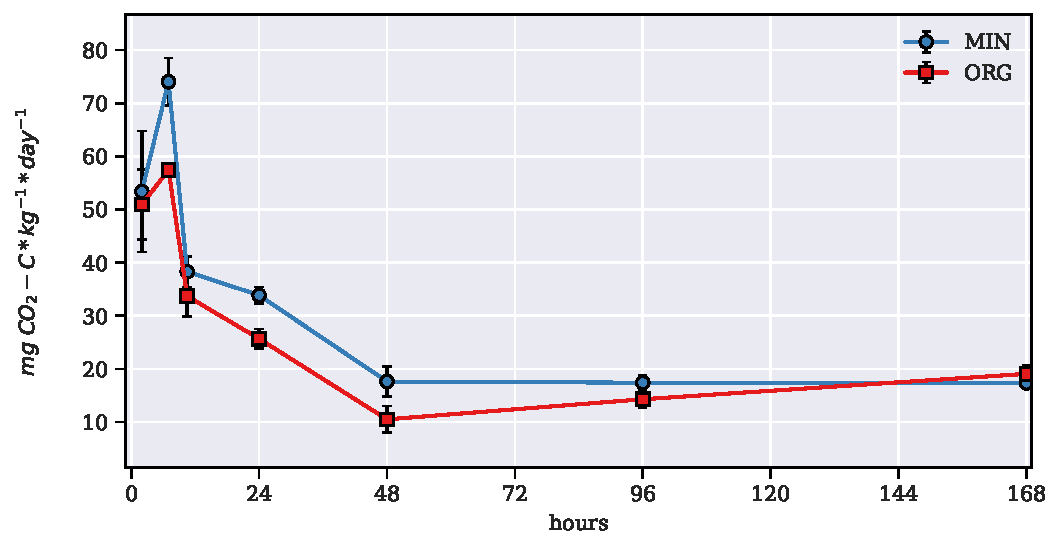
\includegraphics[scale=0.8]{thesis_figures/preliminary/control/Resp.pdf}
			\caption{$CO_2$ respiration as a function of incubation time in non-amended aoil samples of mineral (MIN) and organic (ORG) plots from the Gilat Fertility Experiment}
			\label{fig:resp_control_preliminary}
		\end{figure}
		
		\begin{figure}[H]
			\centering
			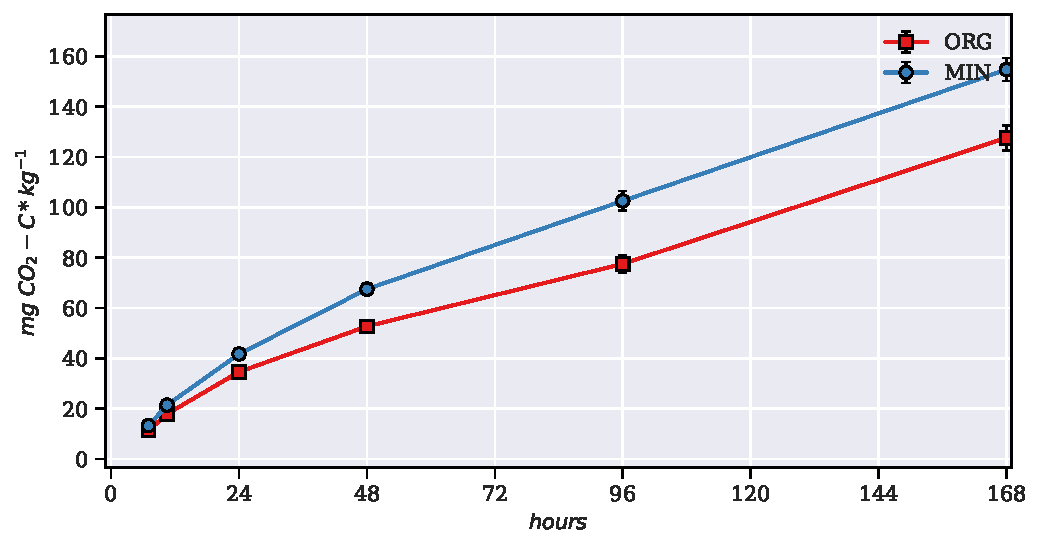
\includegraphics[scale=0.8]{thesis_figures/preliminary/Cum_Resp_CON.pdf}
			\caption{cumulative $CO_2$ respiration  as a function of incubation time in non-amended samples  of mineral (MIN) and organic (ORG) plots from the Gilat Fertility Experiment}
			\label{fig:cum_resp_control_preliminary}
		\end{figure}
		%todo fix comma appears at the begining of the line - before last words of the paragraph
		\noindent A slight increase in MBC (Fig \ref{fig:mbc_control_preliminary}) was observed in Min samples after 24 h of incubation, followed by slight decrease in the next 3 days.  In sharp contrast, in Org samples, MBC had seen a substantial increase of $ \tilde{} $100 \genericunit  between 24-48h of incubation. This increase marked a peak of MBC in Org, after which MBC levels declined sharply to reach a value of ~370 \genericunit, same as in Min.
		
		\begin{figure}[H]
			\centering
			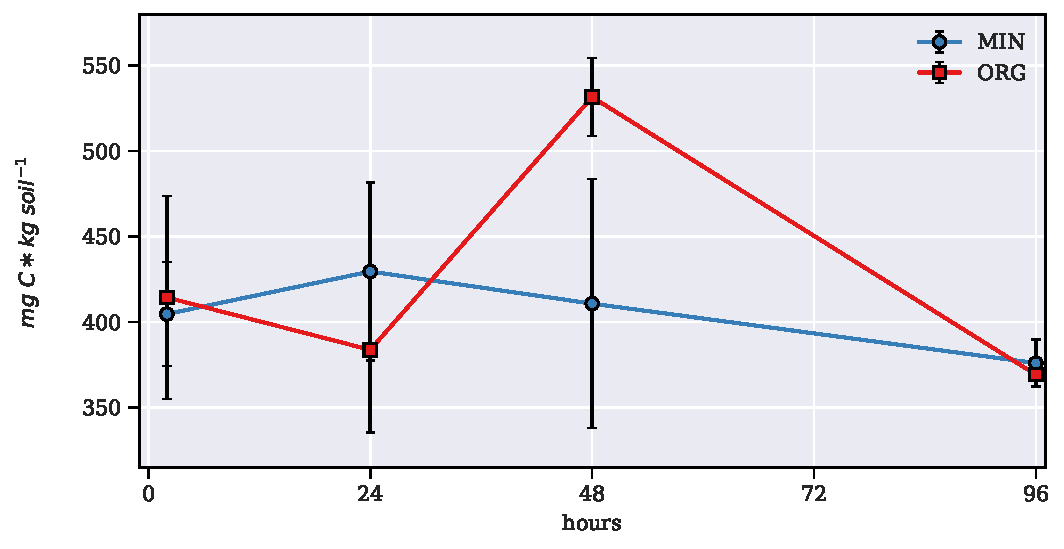
\includegraphics[scale=0.8]{thesis_figures/preliminary/control/MBC.pdf}
			\caption{MBC  as a function of incubation time in non-amended samples  of mineral (MIN) and organic (ORG) plots from the Gilat Fertility Experiment}
			\label{fig:mbc_control_preliminary}
		\end{figure}
		
		\subsubsection{WEOC}
		WEOC  (Fig \ref{fig:weoc_control_preliminary}) was higher in Org throughout the incubation, with the exception of 48h. Initial levels of WEOC were more than 50$\%$ higher in ORG, with this percentage decreasing to ~30$\%$ after 96 h of incubation. In both LTTs, WEOC was almost without change in the first 24 h, subsequently dropping sharply to reach a relatively similar value of ~20 \genericunit in both LTTs after 48 h of incubation. This sharp decrease was followed by a substantial increase in the next 48 h, finally reaching values  slightly, yet significantly higher than initial values. It is worth noting the opposite trends between \hyperref[fig:mbc_control_main]{MBC} and WEOC, particularly in  Org, whereby  a sharp decrease in WEOC between 24-48h, was accompanied by a similarly sharp increase in MBC, and the same (inverse) contrast was observed in the following 48 h.
		
		\begin{figure}[H]
			\centering
			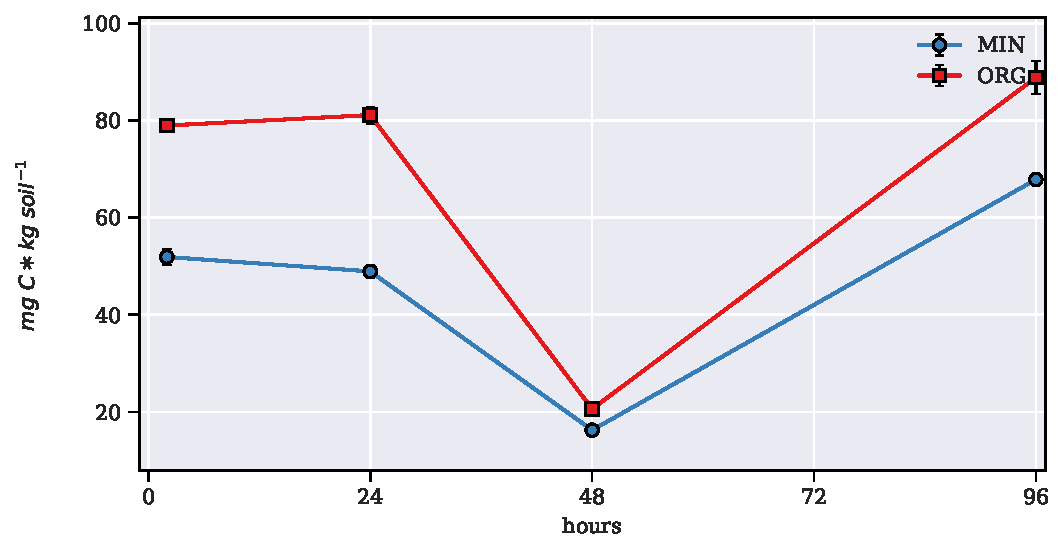
\includegraphics[scale=0.8]{thesis_figures/preliminary/control/WEOC.pdf}
			\caption{WEOC  as a function of incubation time in non-amended samples  of mineral (MIN) and organic (ORG) plots from the Gilat Fertility Experiment}
			\label{fig:weoc_control_preliminary}
		\end{figure}
		
		
		\subsubsection{HWE total Carbon and Carbohydrate-C}
		
		Org had sustained significantly higher levels of HWEC (Fig \ref{fig:hwec_control_preliminary}) and HWES-C (Fig \ref{fig:hwes-c_control_preliminary}) compared with Min throughout the entire incubation, with Org values 50 and 30$\%$ higher than Min, for HWEC and HWES-C respectivly. HWEC and HWES-C had followed very similar patterns throughout the incubation, in both LTTs, while the dynamics of HWEC fluctuated more sharply in the first 96h in Org but not so much in Min which presented strong concurrence in time dependent changes between HWEC and HWES-C (pearson r = 0.97 for first differences in Min, compared with 0.91 for Org, data not shown). These concurrent dynamics suggest that HWES-C comprised a relatively constant fraction of HWEC in control samples of these two LTT, throughout the incubation period. This fraction, calculated by averaging the ratio of HWES-C-to-HWEC across all sampling events, yielded a mean of 0.33 and 0.29 in Min and Org respectively, with a $\pm$0.01 associated error\hiddenTxt{(again data not shown)}.
		
		\begin{figure}[H]
			\centering
			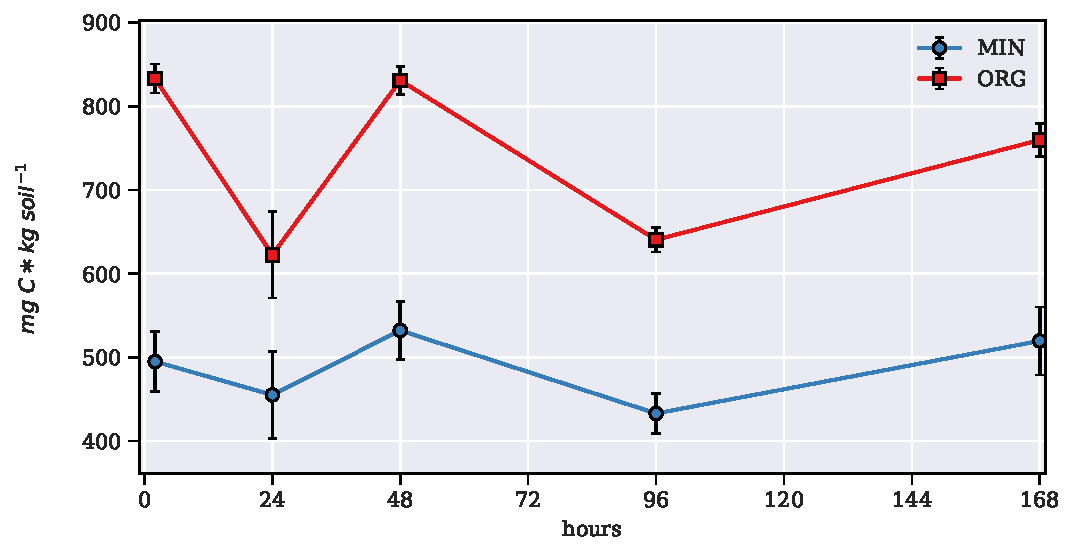
\includegraphics[scale=0.8]{thesis_figures/preliminary/control/HWEC.pdf}
			\caption{HWEC as a function of incubation time in non-amended samples  of mineral (MIN) and organic (ORG) plots from the Gilat Fertility Experiment}
			\label{fig:hwec_control_preliminary}
		\end{figure}
		
		\begin{figure}[H]
			\centering
			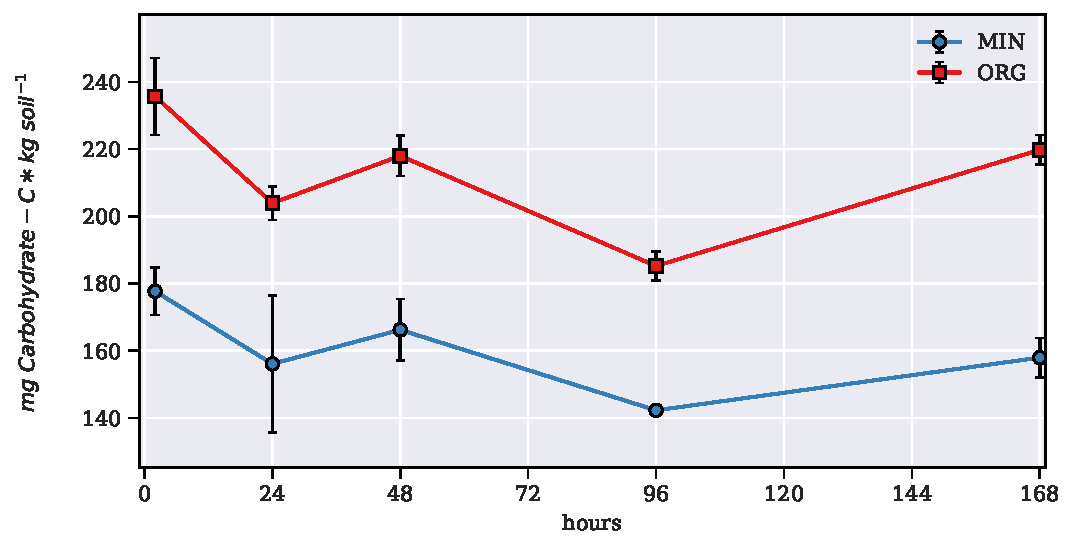
\includegraphics[scale=0.8]{thesis_figures/preliminary/control//HWES-C.pdf}
			\caption{HWES-C  as a function of incubation time in non-amended samples  of mineral (MIN) and organic (ORG) plots from the Gilat Fertility Experiment}
			\label{fig:hwes-c_control_preliminary}
		\end{figure}
		
		\subsubsection{Ergosterol}
		Min presented a slight, insignificant decrease in Erg during the incubation period, with a mean Erg concentration of ~9 \genericunit, while Org sustained a considerable reduction in Erg concentrations from ~13 \genericunit in the first 24 h to 10.5 \genericunit by the end of the incubation (Fig. \ref{fig:erg_control_preliminary}). the ratio of Erg-to-MBC saw some fluctuations in Org during the incubation, yet these were all statistically insignificant. this ratio remained practically steady in MIN samples (Fig \ref{fig:erg_to_mbc_control_preliminary}). the average Erg-to-MBC ratio in ORG and MIN samples was 3 and 2.36\% respectively.
		
		\begin{figure}[H]
			\centering
			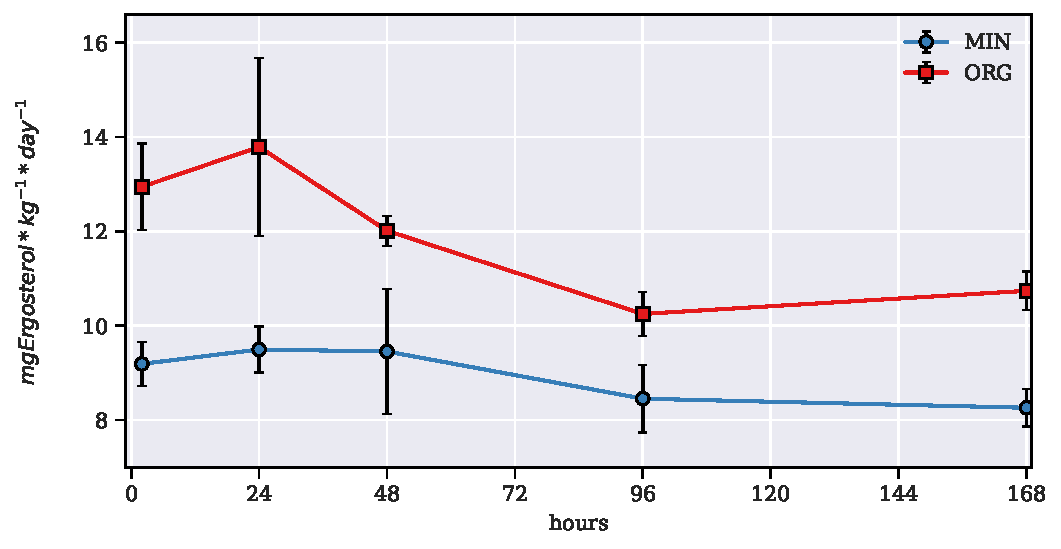
\includegraphics[scale=0.8]{thesis_figures/preliminary/control/Erg.pdf}
			\caption{Ergosterol  as a function of incubation time in non-amended samples  of mineral (MIN) and organic (ORG) plots from the Gilat Fertility Experiment}
			\label{fig:erg_control_preliminary}
		\end{figure}
		
		\begin{figure}[H]
			\centering
			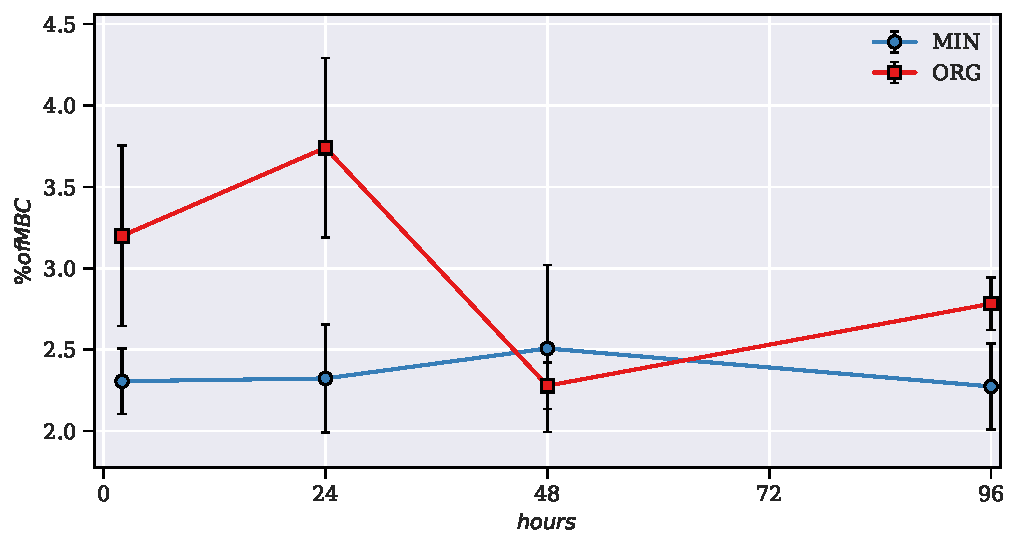
\includegraphics[scale=0.8]{thesis_figures/preliminary/control/Erg-to-MBC_.pdf}
			\caption{Ergosterol-to-MBC  as a function of incubation time in non-amended samples  of mineral (MIN) and organic (ORG) plots from the Gilat Fertility Experiment}
			\label{fig:erg_to_mbc_control_preliminary}
		\end{figure}
		%
		
		\subsection{Dynamics of \gls{som} pools in Straw and Domestic Waste Compost amended soil}
		%todo fix letter symboles overlapping with figure lines in some of the plots
		
		
		\subsubsection{Respiration and MBC}
		%todo change order of figures to fit the text
		%todo cumulative respiration
		Respiration rates and MBC were higher in ORG LTT under both KWC and Str amendment.
		Resp dynamics in the two STTs (Fig \ref{fig:resp_treated_preliminary}) seem to concur with their respective MBC dynamics(Fig \ref{fig:mbc_treated_preliminary}). KWC Resp rates peaked immediately at the onset of the incubation and subsequently decreased rapidly, reaching control normalized values of close to 20 \respunit after 48 hours in both LTTs (Fig \ref{fig:nor_resp_treated_preliminary} B), while STR Resp rates peaked 7 and 10 h after incubation began, in Min and Org respectively (Fig \ref{fig:nor_resp_treated_preliminary} A). Indeed Resp data in KWC is missing for the 7h(as well as 24 h) sampling event, so it is possible that peak rates would have been detected after 7h of incubation. Nonetheless, the substantial difference of more than 150 \genericunit (~75$\%$ ) between the 2h and 10h sampling suggest that, even if this was true, this peak would probably not have been much higher than the observed peak. This intense initial respiration response followed by rapid decline towards Control treatment respiration rates, corresponds  to an initial MBC increase in these KWC amended samples. Similarly, a somewhat delayed Resp peak in STR amended samples and relatively high Resp rates sustained throughout the larger part of the incubation, concur with substantial growth in the first 24 h of incubation as well as with the high levels of MBC sustained through the next 72 h in these samples.\\
		%todo add a note to respiration figure about the different scales in Y axis for Str and KWC amended
		%todo better to put these two plots on the same scale!!!
		\begin{figure}[H]
			\centering
			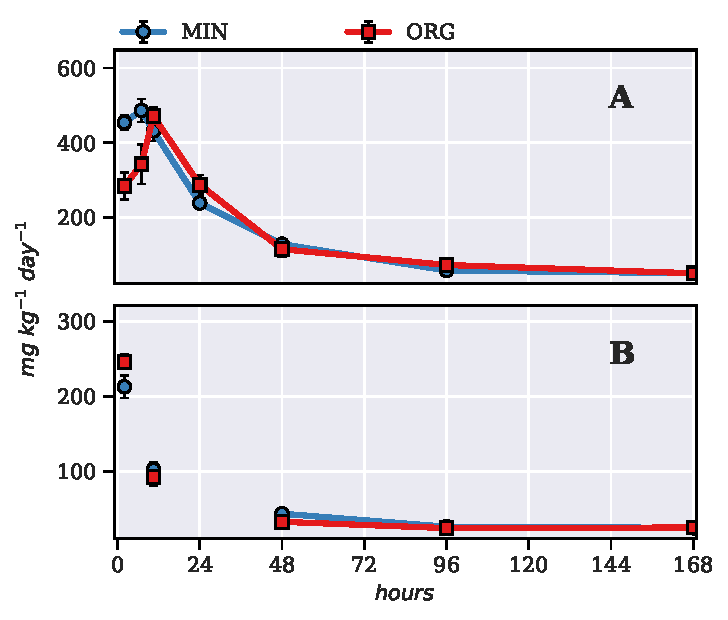
\includegraphics[width=\linewidth]{thesis_figures/preliminary/treated/Resp.pdf}
			\caption{$CO_2$ as a function of incubation time in in STR $\left(A\right)$ and KWC $\left(B\right)$ amended samples of mineral (MIN) and organic (ORG) plots from the Gilat Fertility Experiment}
			\label{fig:resp_treated_preliminary}
		\end{figure}
		
		\begin{figure}[H]
			\centering
			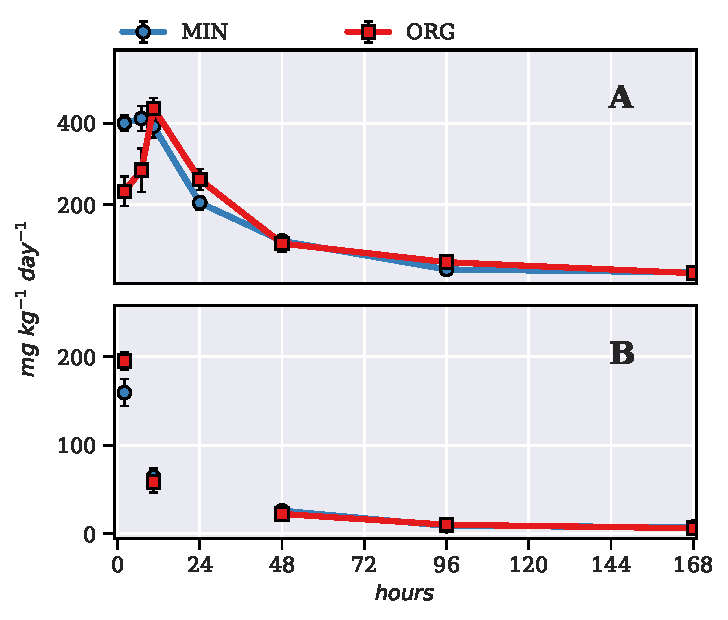
\includegraphics[width=\linewidth]{thesis_figures/preliminary/control_normalized/Resp.pdf}
			\caption{control normalized $CO_2$  as a function of incubation time in in STR $\left(A\right)$ and KWC $\left(B\right)$ amended samples of mineral (MIN) and organic (ORG) plots from the Gilat Fertility Experiment}
			\label{fig:nor_resp_treated_preliminary}
		\end{figure}
		
		\noindent Org had seen an initial increase of 200 and 400 \genericunit MBC over control samples, following the addition of both Str and KWC respectively (Fig \ref{fig:nor_mbc_treated_preliminary}) , while for Min a smaller increase was observed after Str application. Data is missing for Min on the first sampling of KWC  amended samples. Nonetheless, the otherwise parallel MBC trends between the two LTTs ( in KWC amended samples) throughout the rest of the incubation (Fig. \ref{fig:mbc_treated_preliminary}) , suggest a substantial initial increase of ~400 \genericunit over control samples (absolute value of 600 \genericunit MBC at the first sampling)  in Min+STR samples.
		In KWC amended samples, the initial MBC increase (assuming a value of 400 \genericunit MBC$_{Net}$ for Min samples) was followed by a general decrease in both LTTs, suggesting the favorable effect of KWC on MBC,  was short lived, at least in the short-term period recorded in this incubation. Org+KWC had seen a decrease in MBC$_{Net}$ from the initial 382 to 250 \genericunit after 96h of incubation, while Min saw a similar or greater decrease across 4 days of incubation finally reaching a MBC$_{Net}$ value of  110 \genericunit. Moreover, 24 h after the start of the incubation, MBC in Min+KWC samples had decreased by almost 100 \genericunit below the level of corresponding control samples,  suggesting a short-term negative effect of KWC on MBC. In contrast with KWC, STR amendment had initially caused relatively small and little-to-no increases over control samples in Org and Min respectively, while seeing a sharp increase of more than 600 \genericunit in both LTTs after 24 h (~50$\%$ higher than initial increase in KWC amended samples).\\
		
		\begin{figure}[H]
			\centering
			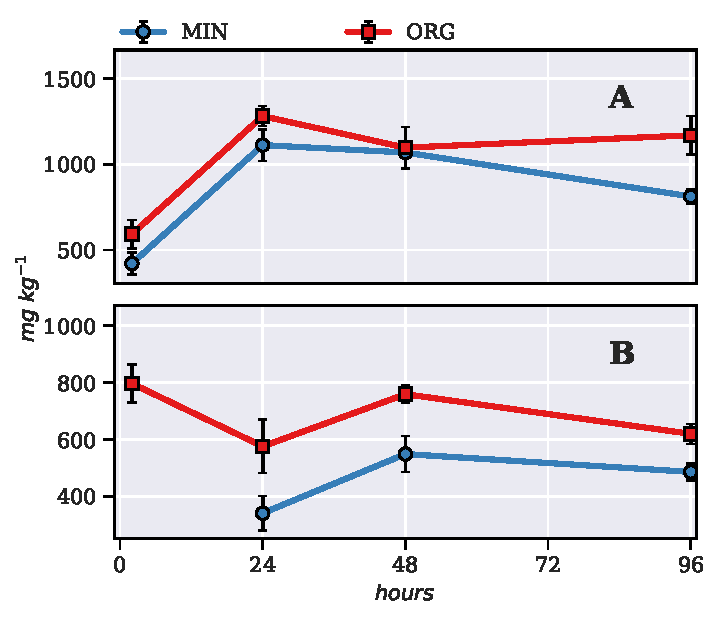
\includegraphics[width=\linewidth]{thesis_figures/preliminary/treated/MBC.pdf}
			\caption{MBC  as a function of incubation time in in STR $\left(A\right)$ and KWC $\left(B\right)$ amended samples of mineral (MIN) and organic (ORG) plots from the Gilat Fertility Experiment}
			\label{fig:mbc_treated_preliminary}
		\end{figure}
		
		\begin{figure}[H]
			\centering
			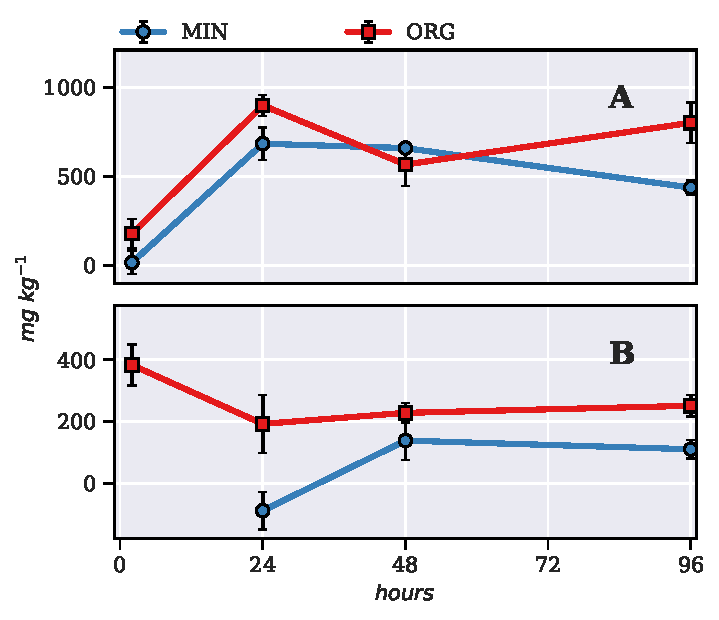
\includegraphics[width=\linewidth]{thesis_figures/preliminary/control_normalized/MBC.pdf}
			\caption{control normalized MBC  as a function of incubation time in in STR $\left(A\right)$ and KWC $\left(B\right)$ amended samples of mineral (MIN) and organic (ORG) plots from the Gilat Fertility Experiment}
			\label{fig:nor_mbc_treated_preliminary}
		\end{figure}
		%thesis_figures/preliminary/treated/Resp.pdf
		
		
		
		\subsubsection{WEOC}
		WEOC dynamics (Fig \ref{fig:weoc_treated_preliminary}) presented a general pattern in all samples, in which the initial increase in WEOC was followed by substantial decline, reaching a minimum level after 48 h and than increasing to varying degrees, depending mostly on STT.  Notably, the decline in WEOC following initial increase was much stronger in STR compared to KWC in the first 24 h, and the overall decrease, in terms of the absolute difference, between the 2h sampling and the 48 h sampling was considerably larger in STR. Additionally, in the last 48 h, KWC samples had increased WEOC levels to values close to initial values, while the corresponding increase in STR was relatively much more limited, with final nor\_WEOC values less than \%30 percent that of initial values. As mentioned earlier for WEOC dynamics of control samples, the WEOC dynamics across the incubation period seem to inversely fit with those of MBC and this observation is made even clearer when considering the variability between the two STTs in this regard. For example, it can be noticed, that in KWC amended samples, MBC levels had seen very little changes in the first 24 h corresponding to the more moderate decrease in WEOC in these samples, compared with the parallel  decrease in STR samples. Similarly, in the last 48 h, a limited increase of WEOC in STR amended samples, corresponds with high levels of MBC while a relatively much larger increase of WEOC in KWC is accompanied by decreasing levels of MBC in these samples.
		\begin{figure}[H]
			\centering
			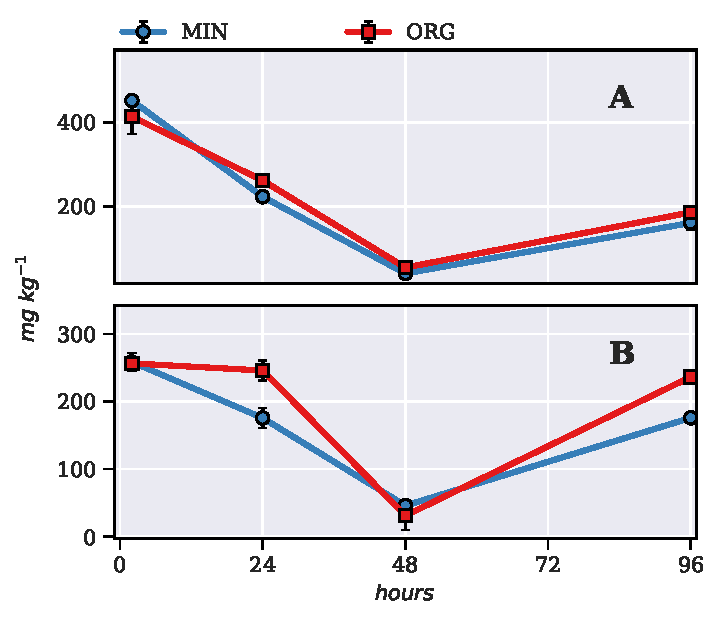
\includegraphics[width=\linewidth]{thesis_figures/preliminary/treated/WEOC.pdf}
			\caption{WEOC  as a function of incubation time in in STR $\left(A\right)$ and KWC $\left(B\right)$ amended samples of mineral (MIN) and organic (ORG) plots from the Gilat Fertility Experiment}
			\label{fig:weoc_treated_preliminary}
		\end{figure}
		similar to microbial biomass and respiration, high WOEC$_{Net}$ (Fig \ref{fig:nor_weoc_treated_preliminary}) values were observed for all treatment combinations in the first sampling. STR amended samples had higher WOEC$_{Net}$ than KWC amended samples, with values  \~{}4 and \~{}8 times higher than control values in Org+STR and Min+STR respectively, compared with \~{}2 and \~{}4 times higher than control in Org+KWC and Min+KWC respectively.
		
		
		\begin{figure}[H]
			\centering
			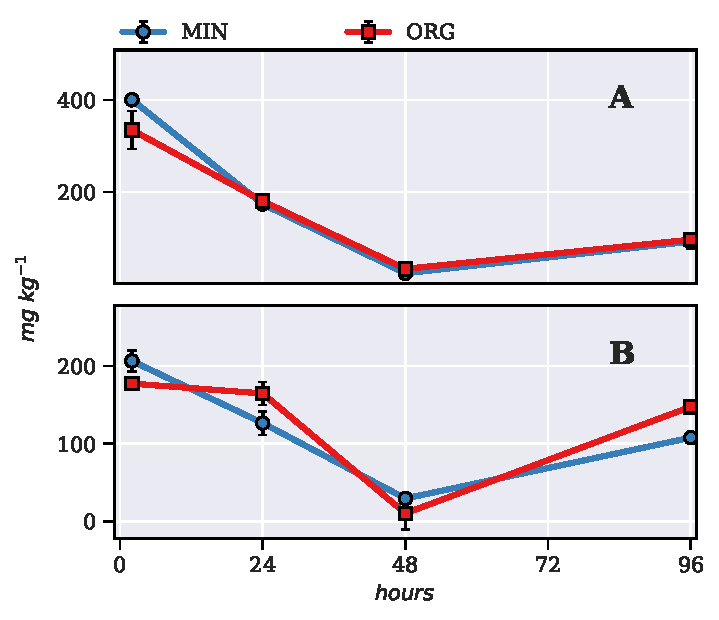
\includegraphics[scale=1]{thesis_figures/preliminary/control_normalized/WEOC.pdf}
			\caption{control normalized WEOC  as a function of incubation time in in STR $\left(A\right)$ and KWC $\left(B\right)$ amended samples of mineral (MIN) and organic (ORG) plots from the Gilat Fertility Experiment}
			\label{fig:nor_weoc_treated_preliminary}
		\end{figure}
		
		
		
		\subsubsection{HWEC and HWES-C}
		In contrast with control samples, where HWEC and HWES levels differed significantly between LTTs during the entire incubation, only few occasions showed significant differences between the two LTTs in STR or KWC amended samples, when results are normalized to control (Fig \ref{fig:nor_hwec_treated_preliminary} and \ref{fig:nor_hwes-c_treated_preliminary}). This may reflect a stronger effect of STTs over the effect of LTTs.
		in Org, KWC and STR had caused relatively small initial increases in HWEC$_{Net}$ and HWES-C$_{Net}$  , while Min amended samples had seen increases of 67 and 95 \% over control samples in KWC and STR amended samples respectively. In KWC amended samples, both Org and Min samples  had seen a reduction of HWEC (Fig. \ref{fig:hwec_treated_preliminary} B) down to levels below those of control samples after 48 h of incubation and these reductions were followed by an increase back to levels comparable to initial values.
		As observed for control samples, an almost constant ratio of HWES-C-to-HWEC was observed in all STT-LTT combinations, excluding the 48h sampling which saw a sharp increase in this ratio for KWC amended samples (in both LTTs). Although the HWES-C-to-HWEC ratio remained mostly constant, it had slightly increased under KWC and even more so under STR .
		
		\begin{figure}[H]
			\centering
			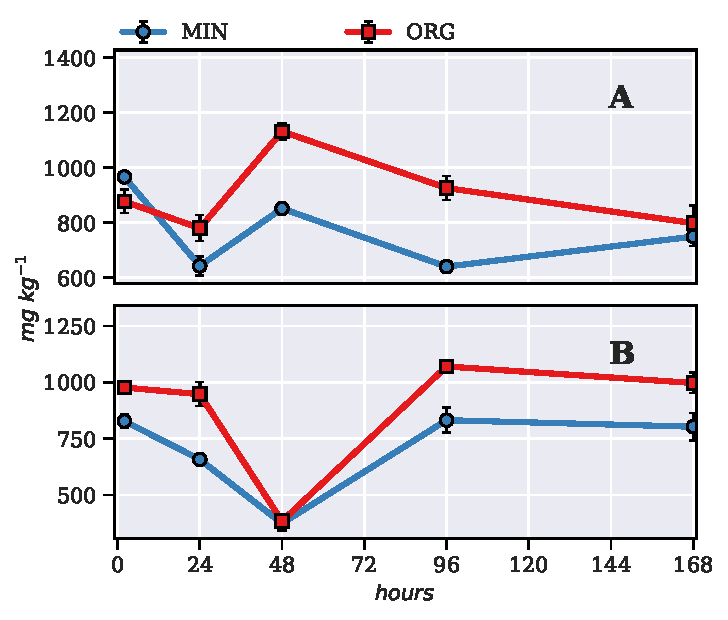
\includegraphics[width=\linewidth]{thesis_figures/preliminary/treated/HWEC.pdf}
			\caption{HWEC  as a function of incubation time in in STR $\left(A\right)$ and KWC $\left(B\right)$ amended samples of mineral (MIN) and organic (ORG) plots from the Gilat Fertility Experiment}
			\label{fig:hwec_treated_preliminary}
		\end{figure}
		
		\begin{figure}[H]
			\centering
			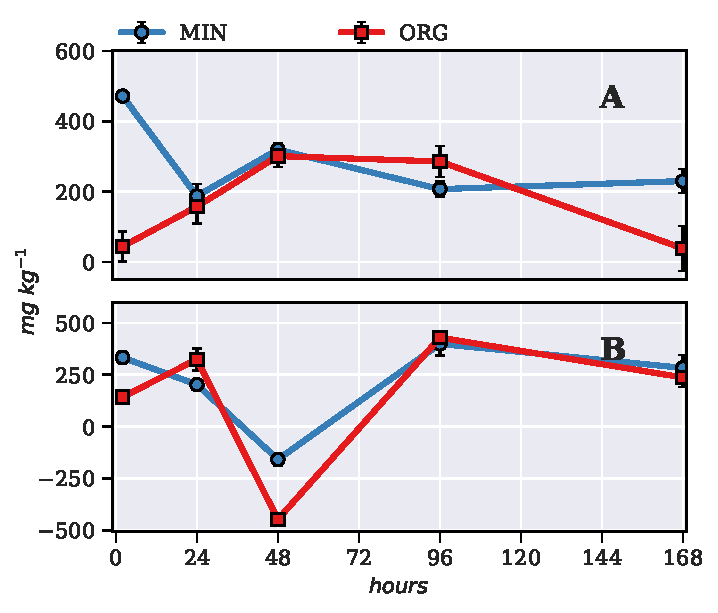
\includegraphics[width=\linewidth]{thesis_figures/preliminary/control_normalized/HWEC.pdf}
			\caption{control normalized HWEC  as a function of incubation time in in STR $\left(A\right)$ and KWC $\left(B\right)$ amended samples of mineral (MIN) and organic (ORG) plots from the Gilat Fertility Experiment}
			\label{fig:nor_hwec_treated_preliminary}
		\end{figure}
		
		\begin{figure}[H]
			\centering
			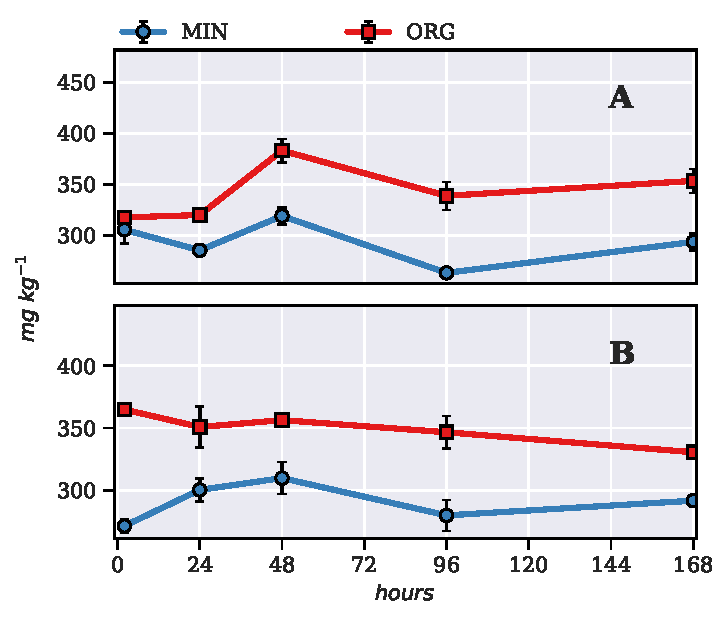
\includegraphics[width=\linewidth]{thesis_figures/preliminary/treated/HWES-C.pdf}
			\caption{HWES-C  as a function of incubation time in in STR $\left(A\right)$ and KWC $\left(B\right)$ amended samples of mineral (MIN) and organic (ORG) plots from the Gilat Fertility Experiment}
			\label{fig:hwes-c_treated_preliminary}
		\end{figure}
		
		
		\begin{figure}[H]
			\centering
			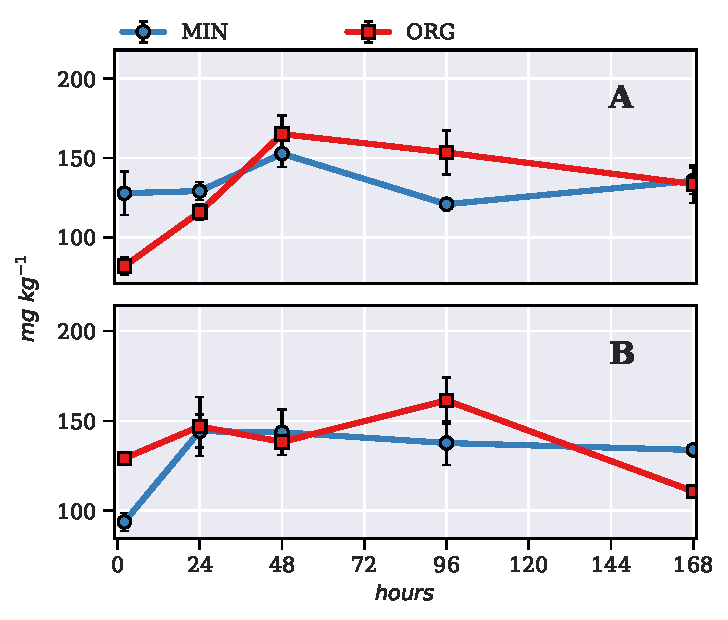
\includegraphics[width=\linewidth]{thesis_figures/preliminary/control_normalized/HWES-C.pdf}
			\caption{control normalized HWES-C  as a function of incubation time in in STR $\left(A\right)$ and KWC $\left(B\right)$ amended samples of mineral (MIN) and organic (ORG) plots from the Gilat Fertility Experiment}
			\label{fig:nor_hwes-c_treated_preliminary}
		\end{figure}
		
		\subsubsection{Ergosterol}
		In STR amended samples (Fig.\ \ref{fig:erg_treated_preliminary}, A), Ergosterol levels rose sharply during the first 96h in both LTTs and remained high up to the end of the incubation. Contrarily, in KWC amended samples (Fig.\ \ref{fig:hwec_control_preliminary}, B), no significant changes were observed throughout the incubation. in STR amended samples, despite the significant increase in ergosterol concentration, no significant increase in Erg-to-MBC (Fig.\ \ref{fig:erg_to_mbc_treated_preliminary} A) over the corresponding values in the control samples, was observed. this was similarly observed for KWC amended samples (Fig.\ \ref{fig:erg_to_mbc_treated_preliminary} B).
		
		\begin{figure}[H]
			\centering
			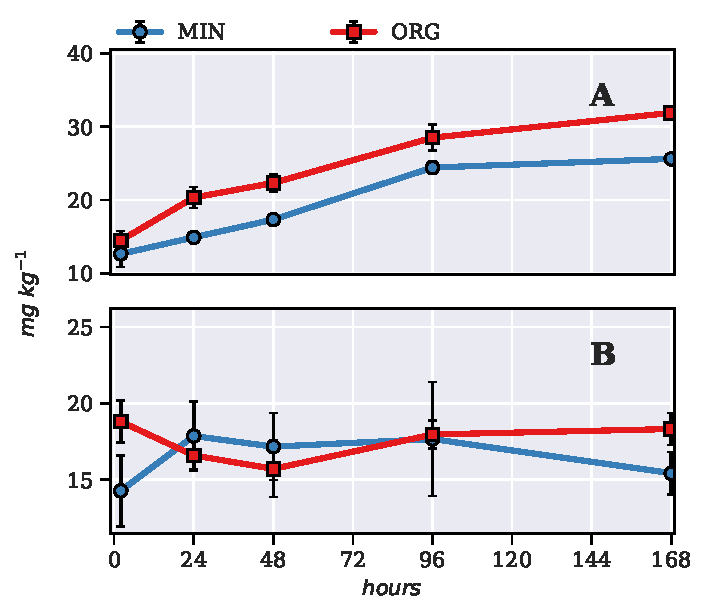
\includegraphics[width=\linewidth]{thesis_figures/preliminary/treated/Erg.pdf}
			\caption{Ergosterol  as a function of incubation time in in STR $\left(A\right)$ and KWC $\left(B\right)$ amended samples of mineral (MIN) and organic (ORG) plots from the Gilat Fertility Experiment}
			\label{fig:erg_treated_preliminary}
		\end{figure}
		
		\begin{figure}[H]
			\centering
			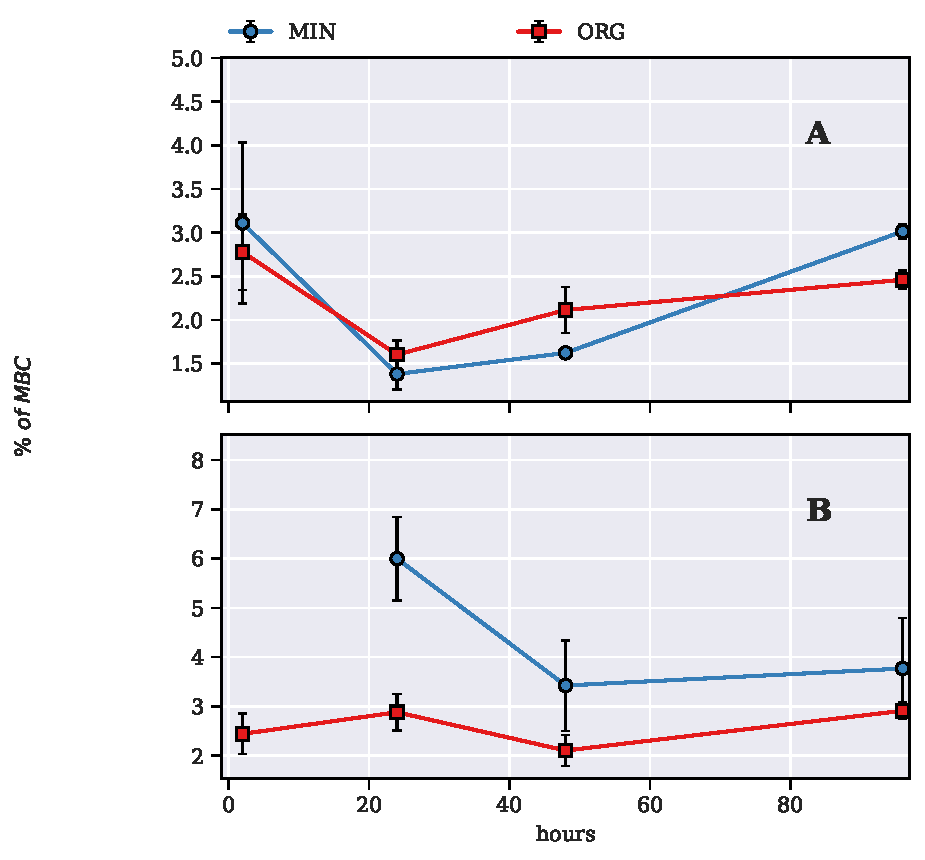
\includegraphics[width=\linewidth]{thesis_figures/preliminary/treated/Erg-to-MBC.pdf}
			\caption{Ergosterol-to-MBC  as a function of incubation time in in STR $\left(A\right)$ and KWC $\left(B\right)$ amended samples of mineral (MIN) and organic (ORG) plots from the Gilat Fertility Experiment}
			\label{fig:erg_to_mbc_treated_preliminary}
		\end{figure}
		
		
		
		
		\section{Incubation with MRE solution}
		%todo in all the figures in this section, refer to water/MRE application marks (grey triangle) in the figure descriptions
		This soil incubation experiment was designed as a 28 days incubation which allowed for a more complete evaluation of the effect of long term fertilization treatments on \gls{som} pools (objective \# 1), compared with the one week  preliminary incubation.\\
		In order to examine the effect of long term treatments on short term dynamics of \gls{som} pools (objective \# 2), a highly labile solution of carbonaceous substances was used, simulating a typical root exudate composition. Root exudates are a major source of energy for the soil microbial community. Labile substrates are rapidly processed by micro-organisms and are considerably more likely to be stabilized as minerally associated \gls{om}. This would enable a more detailed examination of the short term \gls{som} dynamics particularly with regards to substrate stabilization. \\
		MRE was applied in three consecutive pulses in order to examine the interaction between substrate load and soil microbial and pyhsical features and how it affected microbial \gls{cue}. \\
		A third LTT was introduced in this incubation in the form of an unmanaged soil, providing a reference point to which \gls{som} changes in the two other LTT's (ORG and MIN) can be compared.
		In the following section, results for soil parameters that did not include in-week samplings, were presented either as bar plots  or as tables.	weekly MRE/water additions resulted in large in-week fluctuations for the following, frequently sampled for, soil features: MBC, Resp and WEOC (detailed description follows). the remaining soil parameters were only sampled at day 0 and every week end. plotting these later data sets as connected lines implies a known variation for the dynamics between sampling events, which is not necessarily the case. Therefore a bar plot or table representation was preferred.
		
		\subsection{\gls{som} properties in non-amended soil samples}
		
		The first main objective for this work was to establish a reference point  for \gls{som} properties in the three LTTs and evaluate the effect of 5 years of different management histories on the short term dynamics of \gls{som} properties as well as their average baseline values in non-amended samples. As mentioned above, a 4 week incubation was presumed  to better represent the normal fluctuations of \gls{som} pools in a non-amended soil, compared with the results from the shorter, 1 week incubation of non-amended soil which was  included in my preliminary experiment.
		
		
		\subsubsection{short-term dynamics}
		
		the non-amended samples received distilled water as a control for MRE treated samples ( in equivalent volume $=$ 1ml per week).
		each water addition had raised the soil water content by roughly 10$\%$ WHC form 50 to 60$\%$ WHC \pdfcomment[opacity=0.3]{water addition at the begining of each week had raised the water content by about 10\% of Water Holding Capacity}.
		The first water addition was followed by sharp increases in RESP, MBC and  WEOC in all three LTTs (Figures \ref{fig:mbc_control_main}, \ref{fig:resp_control_main} and \ref{fig:weoc_control_main} respectively). Strong pulses of CO2-Respiration were also observed after the 2nd and 3rd water addition. Considerably smaller increases were observed in MBC between days 8-10 and between days 14-15 which seem to have been also related to water additions. These increases following water additions were not observed in WEOC (except for the first water addition). \\
		Regaredless of these pulses, a general trend was observed in the above mentioned parameters, entailing high values during the first part of the incubation (few days to one week depending on the parameter) followed by a decrease and then a steadying of values in later weeks. These similar patterns suggest a connection between microbial growth and activity and the concentrations of WEOC. \\
		Respiration rates rose sharply in the hours following each water addition, peaking after 4h in the 1st and 2nd water additions and after 2h in week 3 (In week 3, no sampling was preformed between 2-12 h after water addition). 4 hours after the first water addition respiration rates were increased by 30$\%$ or more, over the value for 2 h (first sampling), depending on LTT. After A $ \sim $50$\%$ decrease in the next 8 h, rates were mostly  increasing  steadily until the next water addition. The 2nd week saw another, even sharper pulse of respiration, after which respiration rates were constantly decreasing. The 3rd week, similarly saw a sharp increase and then decrease in the first 10 h after water addition and respiration rates subsequently fluctuated within a constant range until the end of that week.\\
		
		\begin{figure}[H]
			\centering
			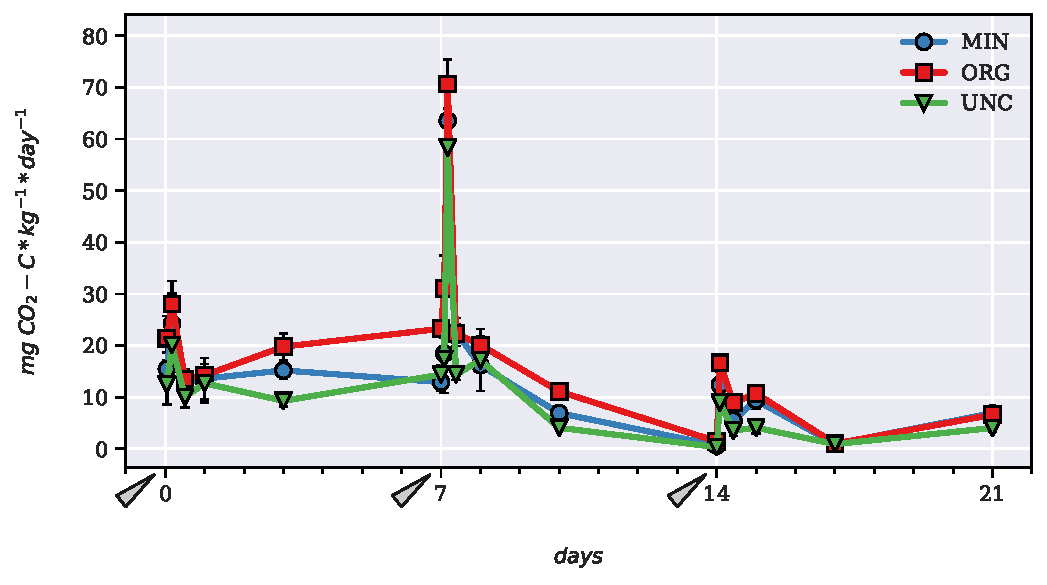
\includegraphics[scale=0.8, width=\linewidth]{thesis_figures/main_incubation/control/Resp.pdf}
			\caption{$CO_2$  as a function of incubation time in non-amended samples of mineral (MIN), organic (ORG) and uncultivated (UNC) plots from the Gilat Fertility Experiment}
			\label{fig:resp_control_main}
		\end{figure}
		\noindent MBC had increased by roughly 10 fold in all three LTTs during the first 24 h. Subsequently, MBC levels dropped rapidly, reaching levels comparable to initial values in all three LTTs by the 8th day. from then on, another, slower and more limited in size increase in MBC was observed for all three LTTs, leveling off in the range of 221-464 \genericunit, by the 10th day. A small but significant increase was again observed during the 14th day (immediately after the 3rd water addition) peaking in at 275-564 \genericunit by day 15 and subsequently decreasing slowly to reach values of between ~200-300 \genericunit by the end of the incubation.\\
		\begin{figure}[H]
			\centering
			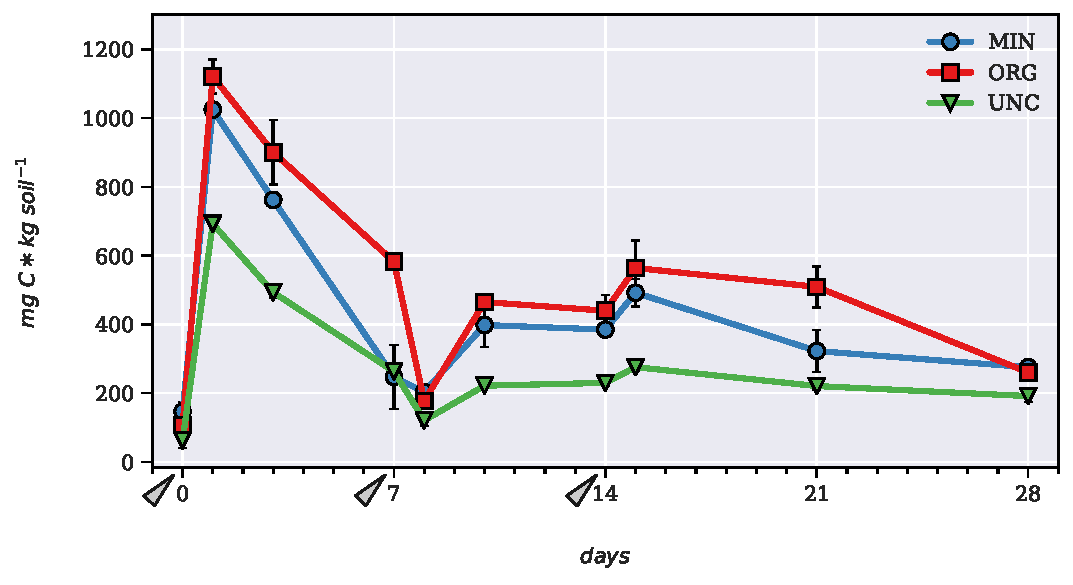
\includegraphics[scale=0.8, width=\linewidth]{thesis_figures/main_incubation/control/MBC.pdf}
			\caption{MBC  as a function of incubation time in non-amendedsamples of mineral (MIN), organic (ORG) and uncultivated (UNC) plots from the Gilat Fertility Experiment}
			\label{fig:mbc_control_main}
		\end{figure}
		\vspace{1cm}
		\noindent Similar to the dynamics of microbial growth and respiration, WEOC  levels had  sharply increased in the first 24 h of incubation (by~300$\%$ in MIN and UNC and ~400$\%$ in ORG), declining considerably during the first half of the 2nd week, and then increasing in the 2nd half and subsequently presenting steady values in the last 2 weeks. In contrast, I did not observe any increases following the 2nd and 3rd water addition, as I did with the dynamics of MBC and particularly those of RESP.  \\
		
		
		\begin{figure}[H]
			\centering
			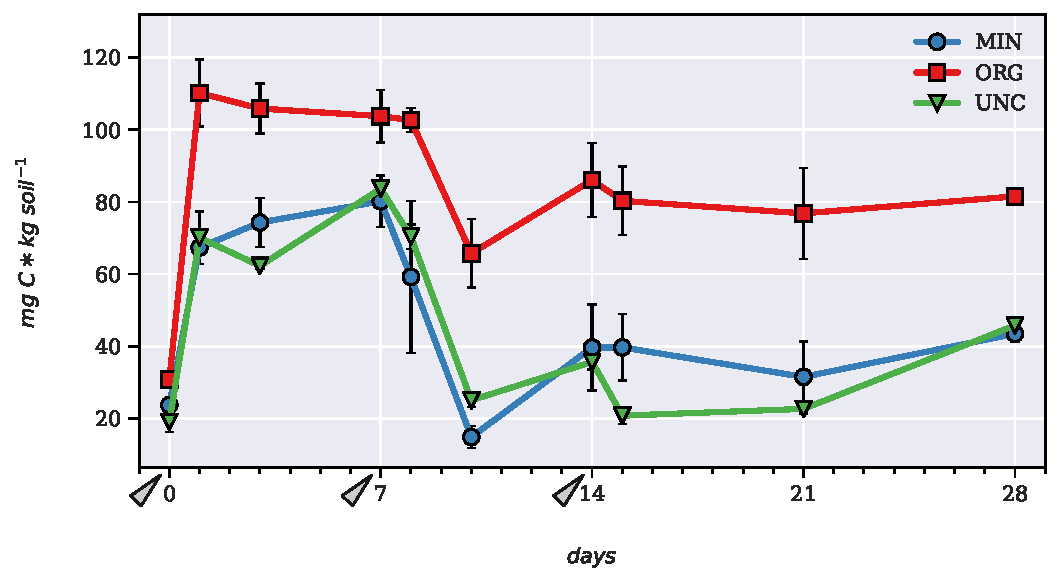
\includegraphics[scale=0.8, width=\linewidth]{thesis_figures/main_incubation/control/WEOC.pdf}
			\caption{WEOC  as a function of incubation time in non-amendedsamples of mineral (MIN), organic (ORG) and uncultivated (UNC) plots from the Gilat Fertility Experiment}
			\label{fig:weoc_control_main}
		\end{figure}
		
		\noindent HWES (Fig. \ref{fig:hwes_control_main}), in contrast with WEOC, showed only slight changes during the incubation, mostly restricted to the first half of incubation, in which a significant decrease ( particularly in MIN and UNC) and then increase back to levels similar to initial values, was observed. HWES remained practically unchanged during the 2nd half of the incubation. Arguably, HWES samplings were limited to the first and last day of each week and it is possible that more pronounced changes would have been recorded for in-week samplings, as for example, was observed for MBC in the first few days of incubation or for WEOC on day 10. Nonetheless, weekly changes in MBC and WEOC were far more considerable compared with those in HWES, with percent changes in the range of hundreds on the 1st week (MBC and WEOC) and  2nd week (WEOC) (Figs. \ref{fig:mbc_control_main} and \ref{fig:weoc_control_main} for MBC and WEOC respectively). \\
		Interestingly, the period where HWES levels decreased (1st week), correspond to a large extent, with the period of increased MBC, CO2-Resp and WEOC.\\
		Aggregate stability (Table \ref{as_main_control}), measured on days 0, 14 and 28, generally decreased throughout the incubation period, except in ORG in the 2nd half of the incubation.
		
		
		\subsubsection{Effect of management history in non-amended samples}
		
		Overall, the level of \gls{som} pools observed for control samples throughout the incubation were in the following order, $ ORG  >  MIN  >  UNC $  , However this pattern was somewhat inconsistent in some of the parameters. HWES values (Fig. \ref{fig:hwes_control_main}) for ORG were significantly and substantially higher than for the two other LTTs on every sampling day and WEOC (Fig. \ref{fig:weoc_control_main}) values significantly differentiated ORG from the two other LTTs on 6 out of 10 sampling events. A similar trend is true also for MBC (Fig. \ref{fig:resp_control_main}) concentrations and RESP (Fig. \ref{fig:resp_control_main}) although differences between ORG and MIN soil  are mostly statistically insignificant and the results are generally not as clear. As mentioned above, MIN had mostly higher values than UNC for most parameters throughout the incubation but this was clear only for HWE-S concentrations, where differences between the two soils are statistically significant on every sampling day.
		%			\myGreen{emphesize that most parameters distinguished LTTs to \gls{som}e degree}\\
		
		\begin{figure}[H]
			\centering
			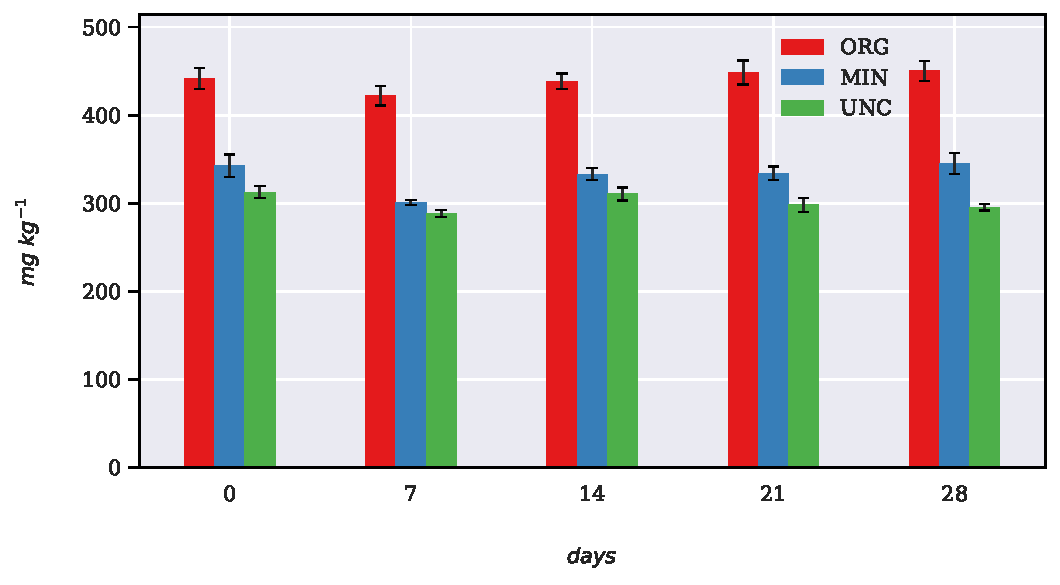
\includegraphics[scale=0.8, width=\linewidth]{thesis_figures/main_incubation/control/HWES.pdf}
			\caption{HWES as a function of incubation time in non-amended samples of mineral (MIN), organic (ORG) and uncultivated (UNC) plots from the Gilat Fertility Experiment}
			\label{fig:hwes_control_main}
		\end{figure}
		
		\noindent Considerable differences were observed between LTTs in cumulative respiration (Fig \ref{fig:cumulative_control_main} ), in the 2nd and particularly in the 3rd week, with the same order generally observed for other parameters, that is ORG $ > $ MIN $ > $ UNC. Total cumulative respiration after 3 weeks of incubation was 154, 199 and 261 in UNC, MIN and ORG respectively.
		\begin{figure}[H]
			\centering
			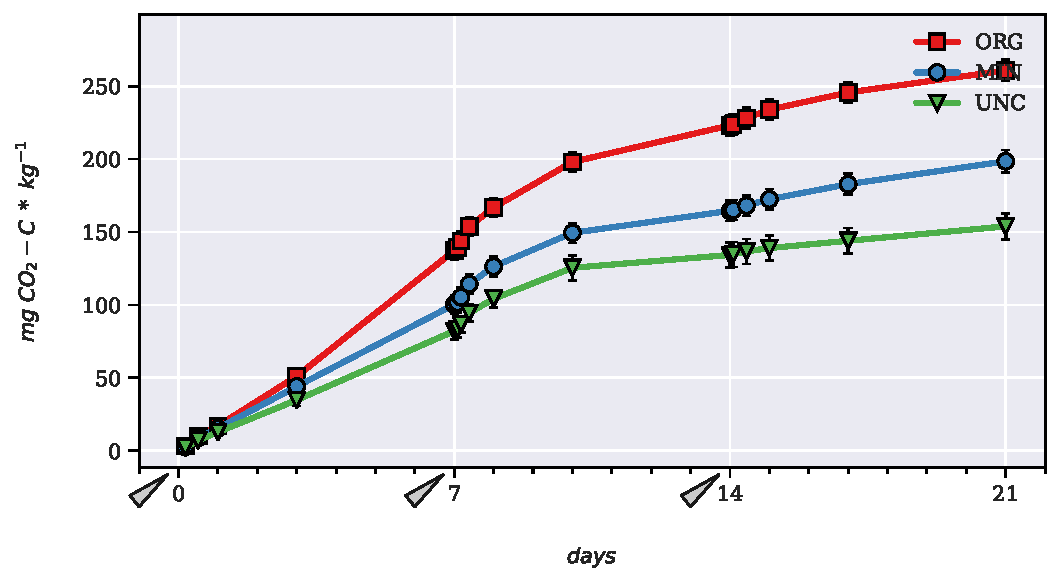
\includegraphics[scale=0.8, width=\linewidth]{thesis_figures/main_incubation/control/Cum_Resp.pdf}
			\caption{Cumulative $CO_2$ respiration  as a function of incubation time in non-amended samples of mineral (MIN), organic (ORG) and uncultivated (UNC) plots from the Gilat Fertility Experiment}
			\label{fig:cumulative_control_main}
		\end{figure}
		\noindent A slight increase in Erg (Fig. \ref{fig:erg_control_main}) was observed for Org and Min during the incubation period while UNC saw an overall slight decrease despite considerable increase in the 1st week . In contrast, Erg as a percent of MBC (Fig. \ref{fig:erg_to_biomass_control_main}) showed a clear reduction in Org and UNC during the 28 days incubation, with most of this decrease occurring in the first half of the incubation. Min samples had seen no significant change in \%Erg of MBC in the course of incubation.
		\begin{figure}[H]
			\centering
			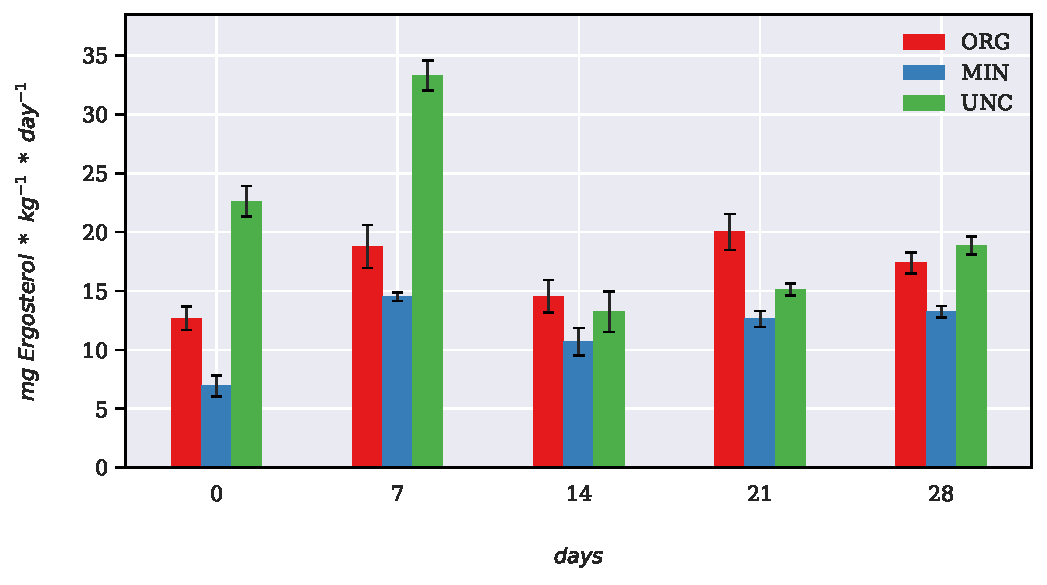
\includegraphics[scale=0.8, width=\linewidth]{thesis_figures/main_incubation/control/Erg.pdf}
			\caption{Ergosterol concentration  as a function of incubation time in non-amended samples of mineral (MIN), organic (ORG) and uncultivated (UNC) plots from the Gilat Fertility Experiment}
			\label{fig:erg_control_main}
		\end{figure}
		
		
		\begin{figure}[H]
			\centering
			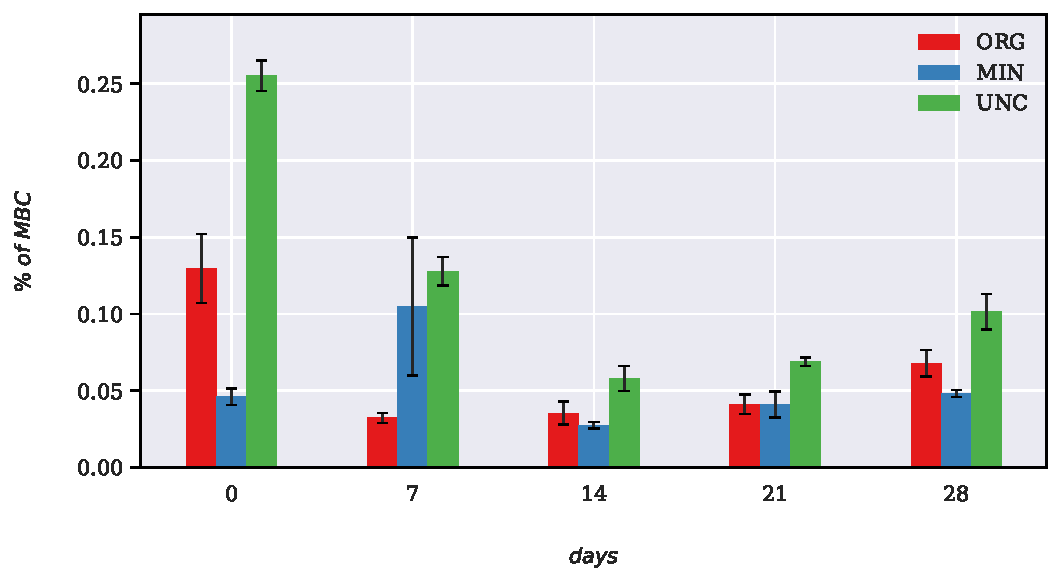
\includegraphics[scale=0.8, width=\linewidth]{thesis_figures/main_incubation/control/Erg-to-MBC.pdf}
			\caption{Ergosterol-to-MBC ratio as a function of incubation time in non-amended samples of mineral (MIN), organic (ORG) and uncultivated (UNC) plots from the Gilat Fertility Experiment}
			\label{fig:erg_to_biomass_control_main}
		\end{figure}
		\noindent as mentioned earlier, the $ \% $WSA (Table \ref{as_main_control}) generally decreased   during the incubation. This was particularly notable in ORG and MIN during the first half of the incubation, with a decrease of more than 5.5\% in both LTTs. A much more limited decrease was observed in UNC during that same period. The total decrease in MIN was roughly double the decrease observed for UNC, while ORG had actually sustained the lowest total decrease in WSA, despite large initial decrease. \\
		%			Strong AS decreases in the first half of the incubation in Org and Min, corresponded to strong microbial activity, compared with the second half of the incubation which showed much smaller decreases (and even an increase for Org) and was incidentally also characterized by a more limited microbial growth and seemingly also microbial respiration ( data for the last week not available).
		%
		
		\begin{table}[H]
\centering
\caption{Aggregate Stability, expressed as \%\gls{wsa}, at $ T_0 $, day 14 and day 28 of incubation, in non-amended samples of mineral (MIN), organic (ORG) and uncultivated (UNC) plots from the \gls{gop}}
\label{as_main_control}
\begin{tabular}{llll}
\toprule
\textbf{soil} &            \textbf{MIN} &            \textbf{ORG} &            \textbf{UNC} \\
\textbf{days} &                &                &                \\
\midrule
\textbf{0   } &  19.33 $ \pm $  0.89 &  18.90 $ \pm $  0.89 &  10.42 $ \pm $  0.81 \\
\textbf{14  } &  13.76 $ \pm $  1.63 &  13.31 $ \pm $  1.59 &   9.44 $ \pm $  1.69 \\
\textbf{28  } &  12.85 $ \pm $  0.94 &  17.01 $ \pm $  0.68 &   6.98 $ \pm $  0.35 \\
\bottomrule
\end{tabular}
\end{table}

		\subsubsection{Baseline}
		\label{Baseline}
		
		Table \ref{baseline_values_of_som_related_properties} shows average values of control samples across day 0 and every week end of the incubation for each LTT (a total of 20 replicates each). Sampling events between week ends were omitted here to eliminate the effect of water additions at the beginning of each week and provide a baseline value that will correspond as accurately as possible to a certain normal level for each parameter-LTT combination.\\
		
\begin{table}[H]
\centering
\caption{Baseline values of SOM pools and associated properties in non-amended soil samples of mineral (MIN), organic (ORG) and uncultivated (UNC) plots from the \gls{gop}}
\label{baseline_values_of_som_related_properties}

\begin{threeparttable}

\begin{tabular}{llllllllll}
\toprule
{} & MBC         &       MBN &      Resp &       HWES &      WEOC &        AS &       Erg &      TOC &      TON \\ 
{} & \scriptsize\genericunit & \scriptsize\genericunit& \scriptsize$ mg\ CO_2$\text{-}$C\ kg^{\text{-}1}\ day^{\text{\text{-}}1}$& \scriptsize\genericunit	& \scriptsize\genericunit & \scriptsize\%WSA& \scriptsize\genericunit& \scriptsize\%weight	& \scriptsize\%weight  \\ \\			
\midrule
ORG &  385.87  a &  49.70  a &  10.43  a &  440.27  a &  75.79  a &  16.69  a &  16.69  b &  1.71  a &  0.15  a \\
MIN &  279.68  a &  50.29  a &   6.81  a &  331.23  b &  43.71  b &  14.95  a &  11.60  c &  1.11  b &  0.09  c \\
UNC &  200.28  b &  32.72  b &   6.79  a &  301.01  c &  41.36  b &   8.81  b &  20.63  a &  1.08  b &  0.10  b \\

\bottomrule
\end{tabular}

\begin{tablenotes}
	\item[*] \scriptsize values represent the mean of replicates sampled throughout the incubation period  (N=20, except for AS, where N=12); Subscript letters represent significance between plots ($ \alpha = 0.05 $). 
\end{tablenotes}

\end{threeparttable}

\end{table}

		\noindent the general order of LTTs described above (i.e. $ ORG > MIN > UNC $) for the 28 days dynamics, was similarly maintained when average baseline values are calculated, though significance between LTTs did differ.
		ORG had a significantly higher baseline value in all measured parameters except Erg compared with UNC, while only MBC, AS, and HWES were significantly different between MIN and UNC.
		Differences between ORG and MIN were significant in TOC, WEOC and HWES, while no significant differences were observed in MBC, CO2-Resp and AS between these two LTTs (although all of these parameters were higher in ORG).
		The lack of significance between ORG and MIN in MBC and CO2-Resp rates, probably reflects, to a large extent, the high degree of variability in the data, due to mostly natural and minor technical sources of variability.  Statistical insignificance between ORG and MIN in AS is more likely to reflect actual closer similarity between these two LTTs, at least when compared with UNC. Differences in AS between ORG and MIN were relatively smaller than those in MBC and CO2-Resp, errors were relatively smaller, and the difference between UNC and the two other soils was roughly 40\% the maximum AS value ( observed in ORG). Thus, it seems that indeed \%WSA, at least for this aggregate size division ( $ >250\mu m$ ), was similar in ORG and MIN.\\
		to summarize, my results suggest that \gls{som} pools in ORG were different from those of the two other LTTs, despite some of these differences not being statistically significant, while MIN and UNC may have been somewhat more similar to each other in terms of \gls{som} pools, than each one of them was similar to ORG. Nonetheless, some properties, particularly AS but also MBC and respiration, suggest a considerable distinction between MIN and UNC. \\
		
		%todo format the table with 0 digits
		
		
		\subsection{Dynamics of \gls{som} pools in MRE amended soils}
		
		The results below are presented with regard to the effect of long term soil management on the short term soil reaction to labile organic input (specific objective \# 2).\\
		
		
		
		\subsubsection{Microbial Respiration}
		
		Similar to MBC (detailed in the following section), CO2-Resp dynamics (Fig \ref{fig:resp_treated_main} ) presented a weekly pulse shortly after each MRE addition, albeit, these pulses were much closer in time to MRE addition than MB growth pulses. In the first two weeks, respiration rates peaked two hours after MRE addition at an average (across LTTs) of 1183 and 623 $mg\ CO2$-$C\ kg^{-1}\ day^{-1}$ respectively, while the last week saw a considerably smaller peak at 246 $mg\ CO2$-$C\ kg^{-1}\ day^{-1}$, which was recorded 10 h after MRE addition (no sampling occurred between 2-10 h).
		The high peak respiration rate in the first week, was followed by a general trend of sharp decrease leading to values close to the final value for that week after 3 days of incubation. The second week, unlike the first week, was characterized by a much smaller peak (roughly half the first peak) as well as higher rates in the following days, compared with a similar time period in the first week. These dynamic entailed a considerably more flattened pattern of respiration in the second week. The third pulse was relatively similar to the 2nd pulse (2nd week) in the general pattern, compared with the first pulse, by having a much more limited peak respiration rate and relatively high rates in the next 24 h.\\
		
		
		\begin{figure}[H]
			\centering
			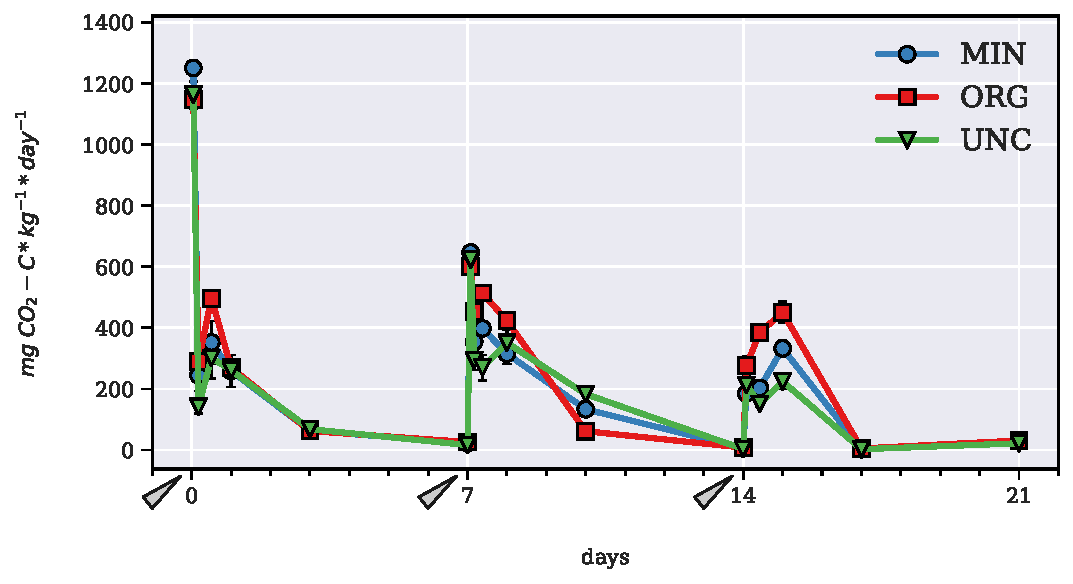
\includegraphics[scale=0.8, width=\linewidth]{thesis_figures/main_incubation/MRE_treated/Resp.pdf}
			\caption{$CO_2$ respiration as a function of incubation time in MRE amended samples of mineral (MIN), organic (ORG) and uncultivated (UNC) plots from the Gilat Fertility Experiment}
			\label{fig:resp_treated_main}
		\end{figure}
		\noindent
		% \myRed{modeling of the general respiration rate dynamics (across all three LTTs) (figure \#), clearly illustrates the changing pattern in respiration between consecutive weeks.
		% 	Using this model for each LTT separately, reveals how these changing patterns between consecutive weeks were differentially  manifested in the different LTTs. This is especially apparent in the second and third weeks. The best fit parameters for each LTT-week with their corresponding stnd error are summarized in table \#}\\
		the average weekly cumulative respiration for all three LTTs (Table \ref{weekly_microbial_growth_and_cumulative_respiration}) rose from 852 \cumrespunit in the 1st week to 1136 \cumrespunit in the 2nd week and than declined again to 659 \cumrespunit in the 3rd week. these weekly values correspond to roughly half or less of the weekly poriton of MRE-C (2200 \genericunit).
		
		
		\begin{figure}[H]
			\centering
			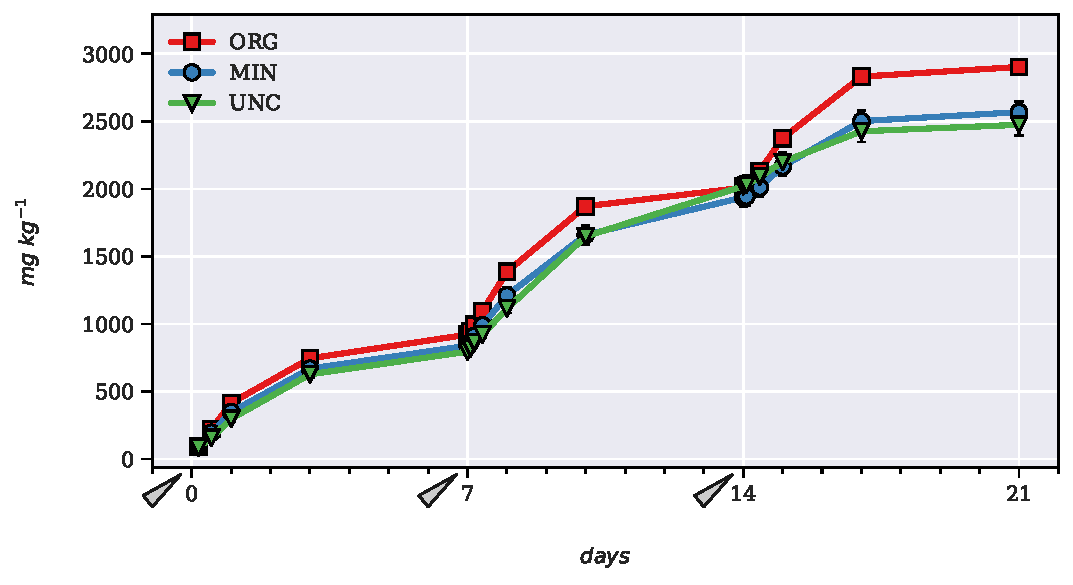
\includegraphics[scale=0.8, width=\linewidth]{thesis_figures/test/Cum_Resp.pdf}
			\caption{cumulative $CO_2$ respiration  as a function of incubation time in MRE amended samples of mineral (MIN), organic (ORG) and uncultivated (UNC) plots from the Gilat Fertility Experiment}
			\label{fig:cum_resp_treated_main}
		\end{figure}
		
		\subsubsection{Microbial Biomass Carbon}
		% todo weekly microbial features table should also include  values as percent of weekly MRE-C.
		%todo check significance between the means (across all LTTs) of each week
		The first addition of MRE had a clear and similar effect on MBC in all three soils, as evidenced from the sharp increase of more than 2000 \genericunit that was recorded in all treated soils 24 hours after the addition (figure \ref{fig:mbc_treated_main}). This increase constituted a peak of MBC in the first ­week (as well as the entire incubation) after which MBC dropped by more than a 1000 \genericunit by the beginning of the 3rd day of incubation. This decrease continued in the next few days, reaching average MBC levels of between 500 and 1000 \genericunit in the MRE treated LTTs by the end of the first week. Questionable data collected on the 8th day of incubation (24 h after the 2nd pulse) and missing data from the 17th day of incubation ( 72 h after the 3rd pulse)  make it hard to assert the precise day of peak MBC in the 2nd and 3rd  week. Nonetheless it is highly plausible that a similar trend as in the 1st week of incubation occurred in these two subsequent weeks in all soils, judging from  the more reliable existing MBC data and from RESP data. Assuming that the dynamics of MBC indeed took on the same shape in the 2nd and 3rd week as in the 1st week, it can be seen that every MRE input is followed by a pulse of microbial growth reflected in the sharp increase and then decrease in MBC and RESP.\\
		
		
		
		\begin{figure}[H]
			\centering
			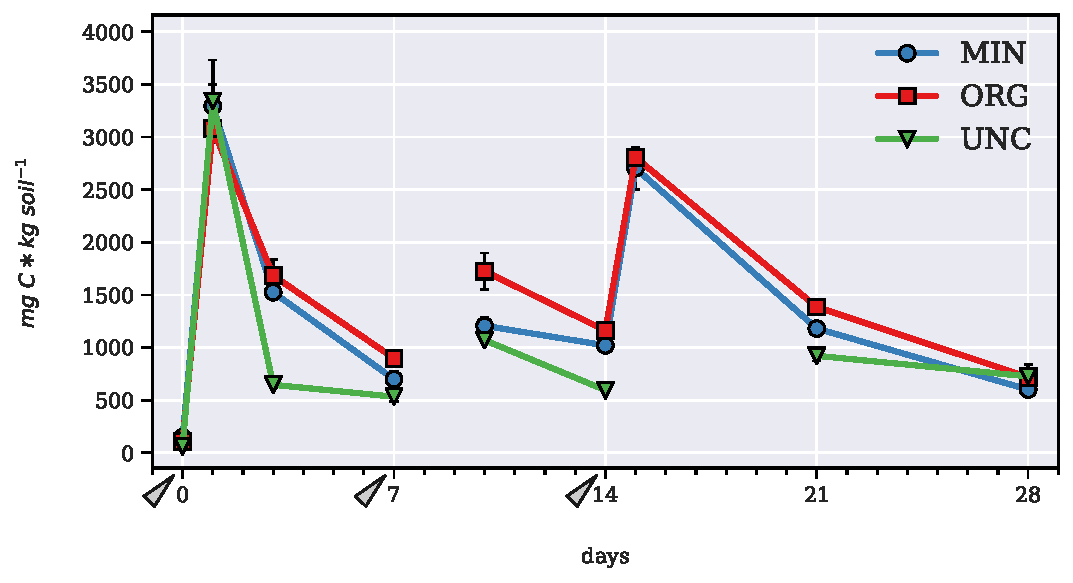
\includegraphics[scale=0.8,width=\linewidth]{thesis_figures/main_incubation/MRE_treated/MBC.pdf}
			\caption{MBC as a function of incubation time in MRE amended samples of mineral (MIN), organic (ORG) and uncultivated (UNC) plots from the Gilat Fertility Experiment}
			\label{fig:mbc_treated_main}
		\end{figure}
		\vspace{1cm}
		\noindent
		the weekly microbial growth in all three LTTs (Table \ref{weekly_microbial_growth_and_cumulative_respiration}) was highest during the 1st week and was then significantly and strongly reduced in the 2nd week,  particularly for ORG and UNC. the 3rd week saw higher growth than in the 2nd week for ORG and UNC but not for MIN. the last week, in which no input was applied, saw substantial negative growth (net decrease in MBC). weekly growth was significantly higher in ORG compared with the two other LTTs in the first week. conversely, ORG saw the strongest negative growth in the last week though this was statistically non-significant. Similar trends as described above are observed for NBC$ _{Net} $.\\
		%todo add units for table
		\begin{table}[H]
\centering
\caption{weekly microbial growth and cumulative respiration, during a 28 days incubation, in MRE amended samples of mineral (MIN), organic (ORG) and uncultivated (UNC) plots from the \gls{gop}}
\label{weekly_microbial_growth_and_cumulative_respiration}
\begin{tabular}{lllrrrr}
\toprule
    && \textbf{week} &           \textbf{1st} &            \textbf{2nd} &           \textbf{3rd} &        \textbf{mean} \\
\textbf{soil} & \textbf{feature} & \textbf{unit}           &              &             &             \\
\midrule
\textbf{MIN} & \textbf{cumulative respiration} & \cumrespunit & 839 &  1097 &  630 &  855\\
    & \textbf{microbail growth} &\genericunit&  552 &   321  & 160 &  344 \\
\textbf{ORG} & \textbf{cumulative respiration} & \cumrespunit & 921 &  1087 &  893 &  967 \\
    & \textbf{microbail growth} & \genericunit & 790 &   264 &  223 &  426 \\
\textbf{UNC} & \textbf{cumulative respiration} & \cumrespunit & 795 &  1224 &  454 &  824 \\
    & \textbf{microbail growth} & \genericunit &   470 &    61 & 326 &  286 \\
\bottomrule
\end{tabular}
\end{table}

		\noindent similar or very close values of MBC were observed for ORG and MIN soils throughout the incubation with ORG exhibiting slightly higher values on most days (significant on day 8 and 21), while MBC dynamics for UNC diverged, at least to some extent from that of the two other soils with significantly lower values observed on the 3rd and 10th day of incubation ( 3rd day of 1st and 2nd week respectively) as well as on the 14th and 21st day of incubation (end of 2nd and 3rd week respectively). Interestingly, by the end of the incubation, absolute MBC values converged to a similar level of roughly 700 \genericunit in all treated soils. compared with pre-incubation values, this value is equivalent to an increase of  roughly 500-600 \genericunit MBC in the treated soils after 4 weeks of incubation.\\
		
		
		
		
		
		\subsubsection{Water Extractable Organic Carbon}
		%todo adjust weoc_pct_change plot: vertical lines for sampling dates;
		%todo LTT markers;
		%todo add extrapolated data point for UNC at day 8 with a dotted line connecting previous and following data point
		
		%todo two seprate plots for WEOC and percent change in cumulative respiration
		Missing WEOC data on the 8th day of incubation prevent a definite description of UNC dynamics in the 2nd week and missing data on the 18th day prevents a detailed description of WEOC dynamics in the the third week for all three LTTs. \hiddenTxt{For day 8, a presumed data point was added based on the trends observed in adjacent weeks.}The dynamics of WEOC (Fig. \ref{fig:weoc_pct_change_treated_main} ) presented an interesting trend which differed significantly between LTTs. The first MRE addition saw a sharp increase of almost 1000 \genericunit in WEOC$_{Net}$ after 24 h in UNC samples whereas only a relatively slight increase of 106 and 33 \genericunit was observed for MIN and ORG respectively. This increase was almost entirely diminished by the 3rd day of incubation in all three LTTs and returned to values very close to the initial values after 7 days. These dynamics were similarly repeated in the 2nd and 3rd weeks, however, WEOC pulses following MRE input increased substantially between subsequent weeks in MIN and UNC. This meant that both the peak of WEOC pulse and its duration (I.e the time period before WEOC returned to baseline level) were increased, with peak WEOC in the second week standing at \~{}500 and \~{}1500 \genericunit for MIN and UNC (assumed) respectively, and these values almost doubled in the third week in MIN. In sharp contrast with these two LTTs, WEOC pulses after each MRE addition in ORG were considerably minor, with peak WEOC in the last week amounting to less than 150 \genericunit.
		These contrasting trends between LTTs, inversely correspond with the respective respiration trends in these LTTs. In the second week of incubation, and still more in the 3rd week, lower respiration clearly corresponded with high WEOC pulse as evident from comparing the rate of change in cumulative respiration with pattern of WEOC (Fig \ref{fig:weoc_pct_change_treated_main}).\\
		considering the intensity of these WEOC pulses immediately following MRE additions, and the above mentioned inverse relation with respiration rates, it seems highly likely that the these sharp increases in WEOC largely represent unprocessed substrate-C.
		%
		\begin{figure}[H]
			\centering
			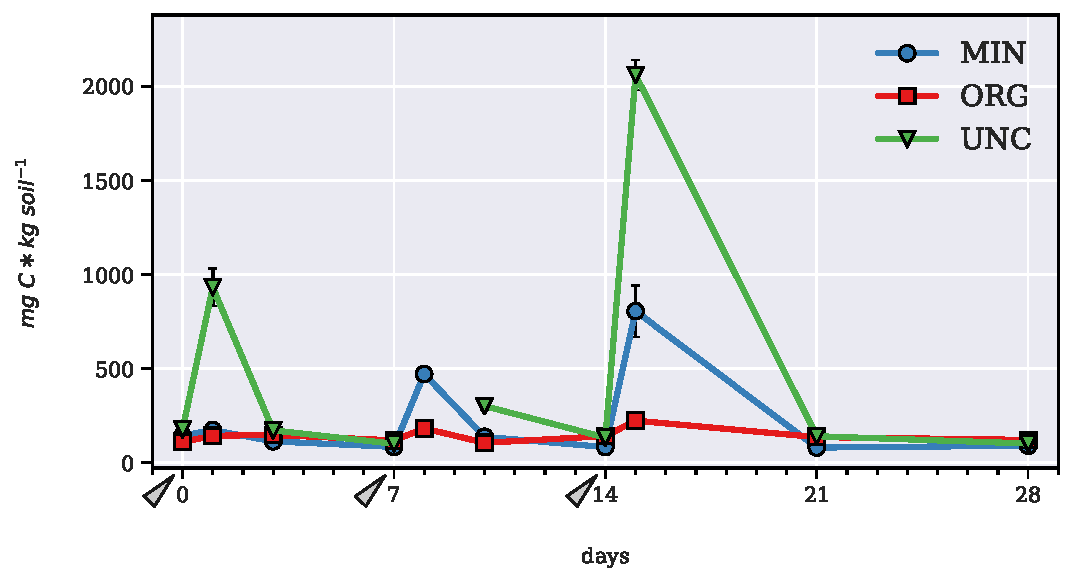
\includegraphics[scale=0.8, width=\linewidth]{thesis_figures/main_incubation/MRE_treated/WEOC.pdf}
			\caption{WEOC as a function of incubation time in MRE amended samples of mineral (MIN), organic (ORG) and uncultivated (UNC) plots from the Gilat Fertility Experiment}
			\label{fig:weoc_treated_main}
		\end{figure}
		
		\begin{figure}[H]
			\centering
			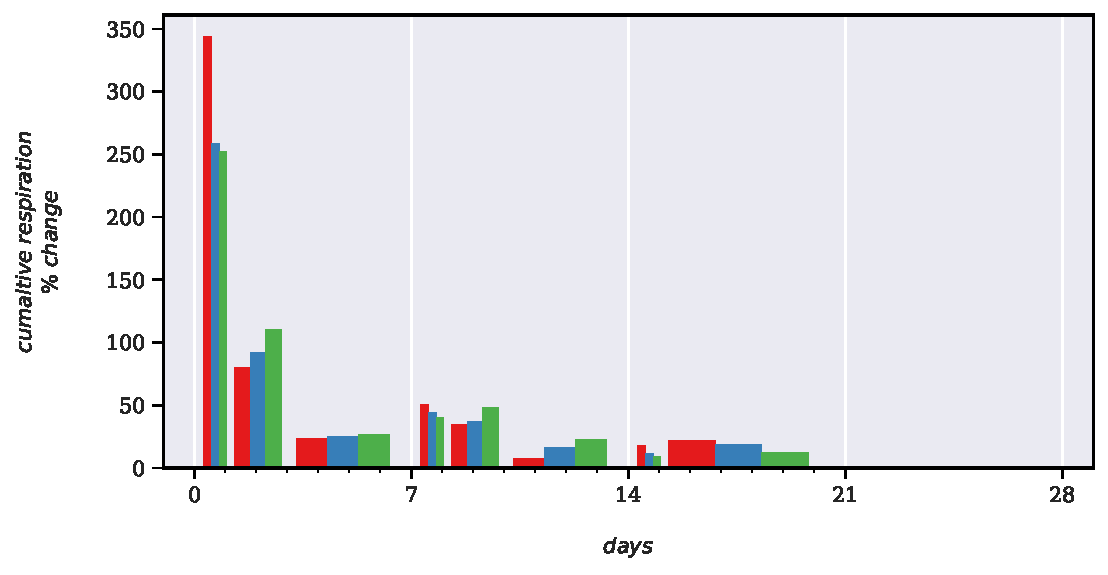
\includegraphics[scale=0.8, width=\linewidth]{thesis_figures/main_incubation/MRE_treated/weoc_pct_change.pdf}
			\caption{Percent change in cumulative respiration for every sampling interval (corresponding to WEOC sampling intervals); Although data is only available for first 3 weeks, plot includes last week of incubation to allow simple comparison with WEOC dynamics.}
			\label{fig:weoc_pct_change_treated_main}
		\end{figure}
		
		\subsubsection{Hot water extractable sugars}
		%todo add net HWES plot
		Throughout the incubation period, ORG maintained highest absolute values of HWES whereas on the final sampling date a comparable level of HWES (roughly 500 \genericunit) was observed for all treated soils (Fig \ref{fig:hwes_treated_main}). ORG  had the highest HWES at the end of the incubation but this result was highly insignificant. UNC and MIN presented similar absolute values of HWES throughout the incubation. This probably reflects, at least to a certain degree their respective \gls{som} stocks compared with ORG as HWES are often correlated with SOC.
		When these results are normalized to the control value (Fig. \ref{fig:hwes_control_normalized_treated_main}), a different prospect of the HWES dynamics emerges, whereby during the first two weeks the three LTTs maintained similar values while the last two weeks saw a clear divergence between UNC and the two other LTTs. The first week saw an increase of 100 \genericunit or less over control values in all three LTTs and the 2nd week saw a similar increase in all three LTTs. In contrast, during the third week, UNC saw a considerable increase of \~{}50 \genericunit in \gls{hwes} while insignificant changes were observed for ORG and MIN. the last week saw a very similar reduction of \~{}50 \genericunit in MIN and UNC and roughly double that reduction in ORG. significant difference was observed between UNC and the two cultivated LTTs on the the last sampling event but not between ORG and MIN.
		
		\begin{figure}[H]
			\centering
			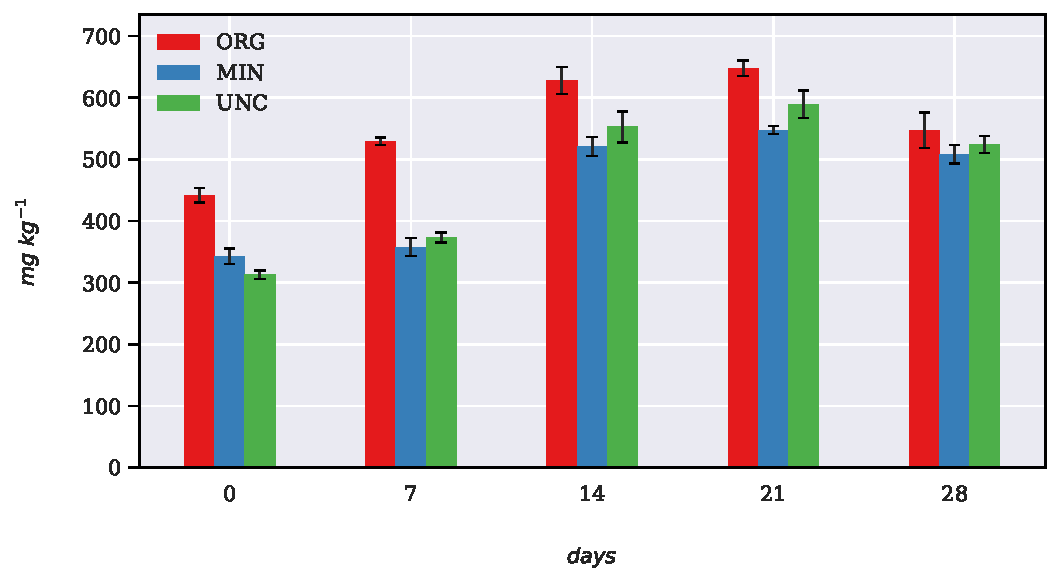
\includegraphics[scale=0.8, width=\linewidth]{thesis_figures/main_incubation/MRE_treated/HWES.pdf}
			\caption{ \footnotesize	HWES as a function of incubation time in MRE amended samples of mineral (MIN), organic (ORG) and uncultivated (UNC) plots from the Gilat Fertility Experiment}
			\label{fig:hwes_treated_main}
		\end{figure}
		
		\begin{figure}[H]
			\centering
			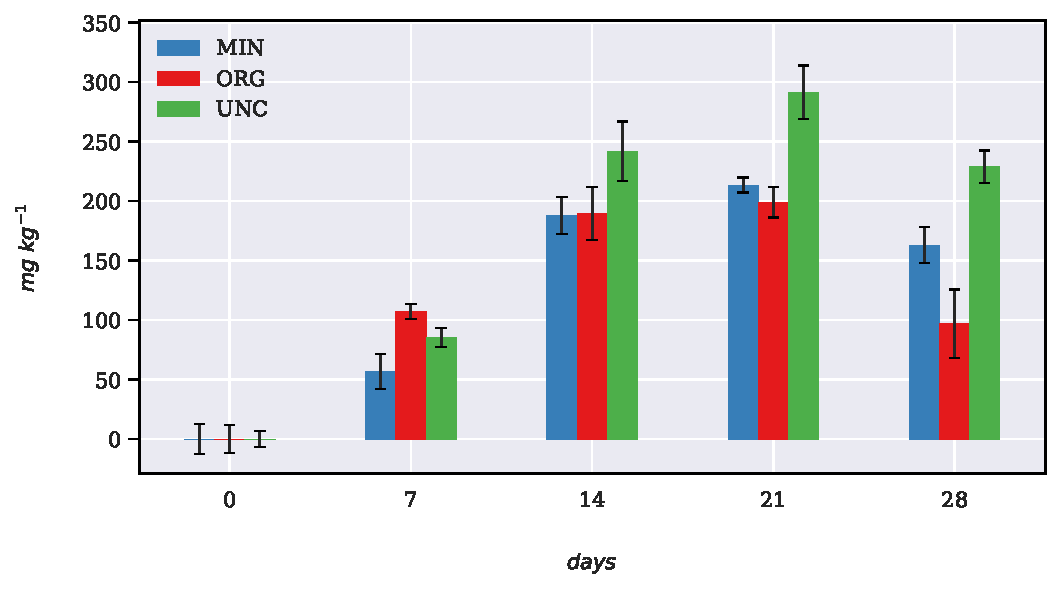
\includegraphics[scale=0.8, width=\linewidth]{thesis_figures/main_incubation/control_normalized/HWES.pdf}
			\caption{HWES normalized to control values as a function of incubation time in MRE amended samples of mineral (MIN), organic (ORG) and uncultivated (UNC) plots from the Gilat Fertility Experiment}
			\label{fig:hwes_control_normalized_treated_main}
		\end{figure}
		
		\subsubsection{Microbial biomass nitrogen and C/N ratio}
		MBN values in MRE treated soils (figure \ref{fig:mbn_treated_main}) ranged between roughly 10 to 150 \genericunit. MBN dynamics for ORG and MIN were similar in general trend. A sharp increase of roughly  7 fold was observed in first two weeks for MIN and ORG soil. In the 3rd week, increases were very small and the 4th week resulted in a slight decrease for MIN and a much larger decrease for ORG bringing the two LTT’ to a similar value of between 80-90 \genericunit.no apparent increase in MBN was observed For UNC in the 1st week. In the 2nd week an increase comparable to that of the two other soils was measured and from then on MBN levels stayed relatively steady, reaching a final value of 60 \genericunit.\\
		%			\myGreen{explain steady MBN in the 1st week for UNC while MBC increased showing extremely high C/N ratio}\\
		Microbial C-to-N ratio ranged from roughly 6 to 11 for the three soils,  throughout the incubation (fig \ref{fig:c_n_ratio_treated_main}), with the highest significant value observed for UNC (11.03) after 3 weeks of incubation.
		An increase in microbial C-to-N ratio over initial value was visible on day 7, 14 and 21 for UNC and ORG while values for MIN stayed relatively steady, with only minor increases in these sampling days. The last week of incubation resulted in a decrease in normalized C-to-N ratio,  especially for UNC and ORG. almost completely undoing the prior increases for MIN, while values for UNC remained relatively high ( differences between MIN and UNC insignificant).
		
		\begin{figure}[H]
			\centering
			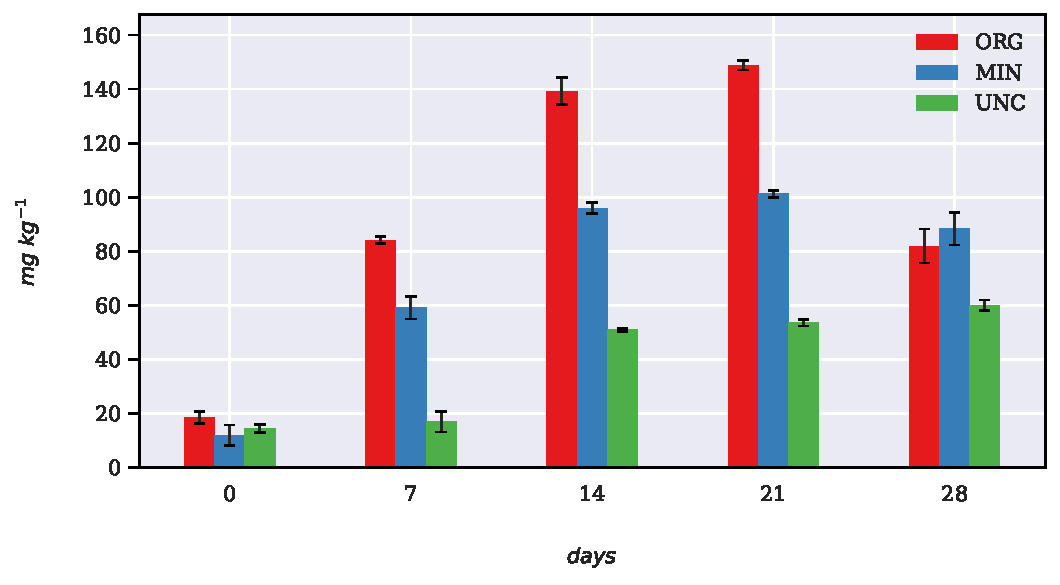
\includegraphics[scale=0.8, width=\linewidth]{thesis_figures/main_incubation/MRE_treated/MBN.pdf}
			\caption{MBN  as a function of incubation time in MRE amended samples of mineral (MIN), organic (ORG) and uncultivated (UNC) plots from the Gilat Fertility Experiment}
			\label{fig:mbn_treated_main}
		\end{figure}
		
		\begin{figure}[H]
			\centering
			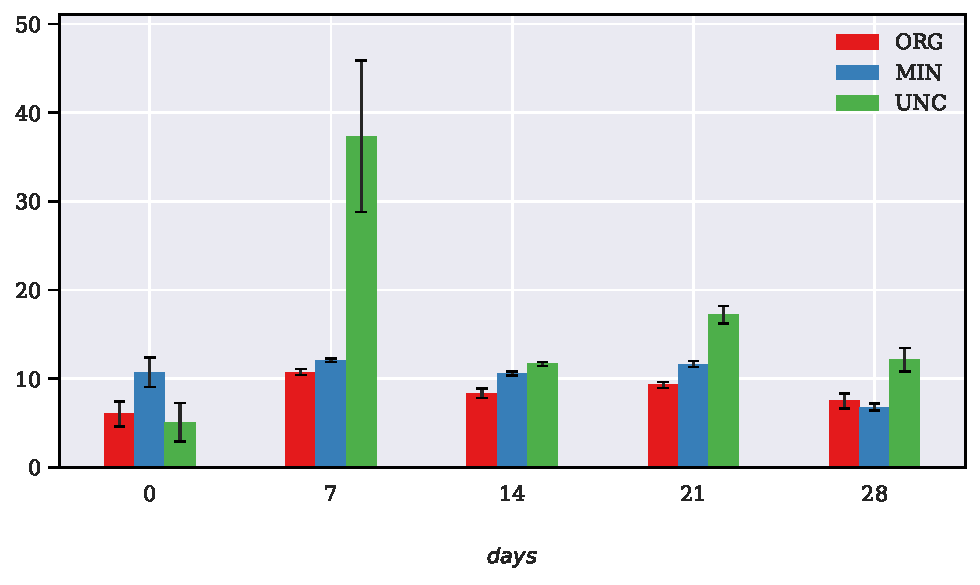
\includegraphics[scale=0.8, width=\linewidth]{thesis_figures/main_incubation/MRE_treated/C_N_ratio.pdf}
			\caption{C/N ratio  as a function of incubation time in MRE amended samples of mineral (MIN), organic (ORG) and uncultivated (UNC) plots from the Gilat Fertility Experiment}
			\label{fig:c_n_ratio_treated_main}
		\end{figure}
		
		
		
		
		
		\subsubsection{Ergosterol-to-microbial biomass (ERG-to-MBC)}
		
		The ratio of ERG-to-MBC dropped sharply in the first week of incubation in both ORG and UNC, with a more moderate decrease in 	MIN, and reached a similar value of  roughly 0.05\% in all three soils. From then onwards, ERG-to-MBC remained relatively steady, with a slight decrease and then increase in the fertilized soils, during the $2^{nd}$ and $ 4^{th} $ weeks respectively. By the end of 4 weeks of incubation,  ERG-to-MBC values were practically identical at \~{}0.03\%, again indicative of the strong effect of MRE treatment compared with the effect of long-term management treatments.
		
		\begin{figure}[H]
			
			\centering
			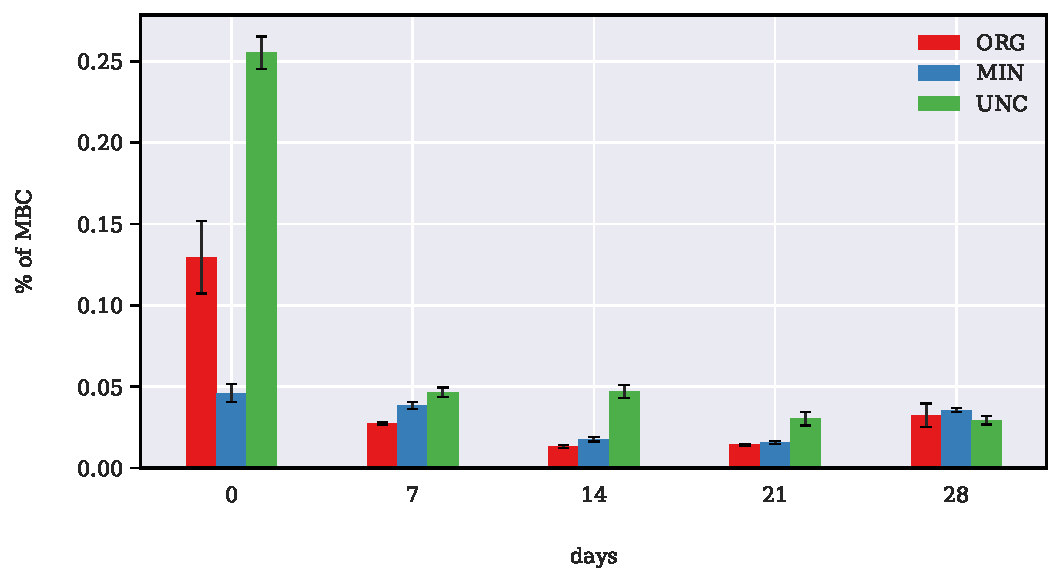
\includegraphics[scale=0.8, width=\linewidth]{thesis_figures/main_incubation/MRE_treated/Erg-to-MBC.pdf}
			\caption{Ergosterol as a function of incubation time in MRE amended samples of mineral (MIN), organic (ORG) and uncultivated (UNC) plots from the Gilat Fertility Experiment}
			\label{fig:erg_treated_main}
		\end{figure}
		
		\vspace{5cm}
		
		\subsubsection{Carbon Use Efficiency}
		The weekly trend in \gls{cue} (Table \ref{cue_treated_main}) seemed to differ between the cultivated LTTs and the non-cultivated LTT. Both cultivated LTTs presented a sharp decrease of \~{}50\% in \gls{cue} between the 1st and 2nd week with values staying practically the same between the 2nd and 3rd week. by contrast UNC saw an even more pronounced decrease in \gls{cue} between the 1st and 2nd week (about 10 fold) while the 3rd week actually saw a sharp increase compared with the 2nd week, with a \gls{cue} similar to that observed in the 1st week.
		
		
		\begin{table}[H]
\centering
\caption{weekly Carbon Use Efficiency during first three weeks of the incubation, in MRE amended samples of mineral (MIN), organic (ORG) and uncultivated (UNC) plots from the \gls{gop}}
\label{cue_treated_main}

\begin{threeparttable}


\begin{tabular}{llll}
\toprule
\textbf{soil} &           MIN &           ORG &           UNC \\
\textbf{week} &               &               &               \\
\midrule
\textbf{1   } &  0.40 $ \pm $  0.06 &  0.46 $ \pm $  0.02 &  0.37 $ \pm $  0.04 \\
\textbf{2   } &  0.23 $ \pm $  0.06 &  0.20 $ \pm $  0.03 &  0.05 $ \pm $  0.04 \\
\textbf{3   } &  0.20 $ \pm $  0.07 &  0.20 $ \pm $  0.05 &  0.42 $ \pm $  0.07 \\
\bottomrule
\end{tabular}

\begin{tablenotes}
	\item[*] \scriptsize values represent a mean of 4 replicates along with standard error;
\end{tablenotes}

\end{threeparttable}

\end{table}

		
		
		\subsubsection{Aggregate stability}
		
		Aggregate stability was measured three times during the incubation, at $ T_0 $, day 14 and day 28. The percentage of stable aggregate was increased by more than 20\% in the course of the incubation in all three soils (Table \ref{as_main_treated}). For ORG and UNC, \~{}80\% of the stable aggregates formed during the incubation period were formed in the first half of the incubation, while MIN samples presented almost similar increases in percentage of stable aggregates in the second half as in the first half of incubation. UNC had the lowest value of \%WSA in all three samplings.\\
		
		\begin{table}[H]
\centering
\caption{Aggregate Stability, expressed as \%\gls{wsa}, at $ T_0 $, day 14 and day 28 of incubation, in MRE amended samples of mineral (MIN), organic (ORG) and uncultivated (UNC) plots from the \gls{gop}}
\label{as_main_treated}
\begin{threeparttable}
\begin{tabular}{llll}
\toprule
\textbf{soil} &            MIN &            ORG &            UNC \\
\textbf{days} &                &                &                \\
\midrule
\textbf{0   } &  19.33 $ \pm $  0.89 &  18.90 $ \pm $  0.89 &  10.42 $ \pm $  0.81 \\
\textbf{14  } &  31.87 $ \pm $  2.72 &  36.71 $ \pm $  1.69 &  28.30 $ \pm $  2.45 \\
\textbf{28  } &  45.47 $ \pm $  1.92 &  41.57 $ \pm $  1.49 &  34.04 $ \pm $  1.81 \\
\bottomrule
\end{tabular}

\begin{tablenotes}
	\item[*] \scriptsize values represent a mean of 4 replicates along with standard error;
\end{tablenotes}

\end{threeparttable}
\end{table}

		
		
		%		\begin{figure}[H]
		%			\centering
		%			\includegraphics[scale=0.8]{thesis_figures/main_incubation/MRE_treated/\gls{cue}.pdf}
		%			\caption{\gls{cue} in MRE amended samples}
		%			\label{fig:cue_treated_main}
		%		\end{figure}
		%
		

	\chapter{Discussion}
		% !TeX root = ../main.tex
		
		% questions for Asher
		% 1. references for the idea that variabilty is inherntly greater in biologicL rather than chemical or physical tests.
		%todo TOC/SOC, our/my, we/I
		
		
		%\section{Preliminary incubation}
		
		\section{effect of management history on \gls{som} pools in non-amended soils}
		
		\subsection{Cultivated compared with non-cultivated}
		%todo how to cite this 'Seven-years of productivity and potential fertility in organically managed...' (ask Asher)
		Despite my expectations, both cultivated LTTs and especially ORG had resulted in higher baseline values for most parameters, compared with the non-cultivated LTT. Although agricultural intensification and long term fertilization has been repeatedly shown to diminish overall soil health and cause a reduction in \gls{som}, compared with non-cultivated soils \citep{laurance2014, mganga2016, tilman2011}, there is some evidence pointing out that this is not necessarily the case for certain agricultural management scenarios, particularly in arid and semi-arid environments.  For example, \citet{trivedi2016}, in a meta analysis, found that in arid climates, cultivated soils had on average significantly higher values of SOC compared with unmanaged soils. Similarly, repeated analysis of a large data base from soils in the US great plains area, revealed that SOC loss due to cultivation was lowest in low rainfall areas ($ \sim $300 mm MAP)\citep{miller2004, burke1989}. \citet{paz-kagan2014} conducted a research that included soils from the Migda research farm (\~{}30 km from the Gilat Research Center, with similar climatic conditions and soil properties), and found no significant improvement in Soil Quality Index(SQI) (including soil parameters such as \gls{soc}, hydraulic conductivity and surface hardness) when transitioning between agricultural land use and a natural ecosystem management. \citet{garcia-orenes2010} found no significant decrease in soil health parameters (TOC, WEOC, MBC, basal respiration) compared with an adjacent abandoned field (some natural vegetation cover) in soils from SW Portugal, treated for one year by  a number of different agricultural practices, including tillage and herbicide use. Although these different treatments were each tested separately (e.g compare tilled soil to non-cultivated soil),as opposed to combined long-term treatments in the current work (e.g. compare conventional management to unmanaged soil ), and lasted for only one year, nonetheless, the outcome of this work, clearly support the notion that certain agricultural practices may not have a detrimental effect on overall soil health when compared with non-cultivated soils in a semi-arid climate context. indeed some practices - in the case García-Orenes’s work, the return of substantial amount of oat straw – can actually cause a significant improvement in soil health parameters, not just compared with a non-cultivated soil but also compared with a natural cover soil ( Mediterranean woodland ).\\
		My results provide additional evidence supporting a similar line of evidence. Five years of intense compost application ( $ 6 m^3*year^{-1} $ ) combined with an otherwise conventional management system (Org), increased TOC by almost 60\% over an adjacent uncultivated soil (UNC). Org had also resulted in increased baseline levels of \gls{som} pools such as MBC, WEOC  and HWES-C  as well as higher basal RESP and higher AS, compared with UNC. \\
		Evidence from a number of experiments and review analysis, suggest that the net energy influx into the soil ecosystem from plants, can act as a key factor determining the rate and direction of changes in \gls{som} pools  and AS, when comparing cultivated and non-cultivated soils. \\
		Net primary productivity (NPP) is the net solar energy accumulated by vegetation per unit area and unit time. it is an important proxy of ecosystem function and carbon sequestration capacity\citep{jackson2016}. High NPP levels are likely to increase, besides plant biomass, the allocation of plant carbon and nutrients as root deposits, thus enriching the soil with labile, easily stabilized \gls{om}.  \\
		\citeauthor{trivedi2016}, compared cultivated and non-cultivated soils in the four major climatic regions of the world, and found NPP to be higher for non-cultivated soils in temperate and tropical climates and oppositely lower for non-cultivated soils in arid ecosystems. concurrently these trends where in accordance with SOC trends in soils from these two types of ecosystems, indicating the connection between the build-up of \gls{som}  and ecosystem productivty. \citet{bhardwaj2011} presented direct evidence relating the improvement in soil quality indices to increased NPP, when examining a set of long-term intensively managed row crop systems in the upper Midwest part of the USA.\\
		Considering the marked differences in management inputs between the cultivated and non-cultivated LTTs in the Gilat Organic Plots(GOP), in the form of water, fertilization and seeding, it is very possible that substantial differences in NPP between these two management systems occurred in various periods, especially during the long dry summers typical in this area, in which little  if any significant plant growth is expected in non irrigated soils. \\
		In light of these evidences, it is possible that differences in NPP between the cultivated LTTs and the non-cultivated LTT used in the current experiment, may have been at least partly responsible for the observed differences in \gls{som} related properties.
		This supposition is further supported by field observations and fertility tests from the GOP, where significantly higher crop yields were observed in ORG compared with MIN in various time points \myRed{* (\textit{Seven-years of productivity and potential fertility in organically managed Mediterranean Vertisol and semi-arid Loess soils})}. Although data for the complete calculation of NPP is missing in this long-term experiment, it is conceivable that higher crop yields were also expressed as higher NPP, eventually resulting in increased SOC (and related properties) accrual, an outcome that was observed in the current experiment. The \myRed{\textit{Seven-years of productivity and potential}} also reported increased weed coverage in Org compared with Min. This may have been an additional factor contributing to increased organic matter input in these plots.\\
		The possible importance of NPP in controling long term \gls{som} dynamics in these LTTs is in accordance with the latest emerging concepts of \gls{som} formation and preservation (\textit{ soil continuum model} ) as these views emphasize the role of a continuous flux of labile organic substances into the soil as a key feature in sustaining high levels of \gls{som} \cite{kleber2010, lehmann2015}.
		
		\subsection{Organic vs. chemical long-term fertilization}
		%todo find references for high variability in biological systems
		I expected 5 years of organic fertilization to increase \gls{som} pools over mineral-only fertilization, and indeed baseline TOC, WEOC and HWES (and HWEC, as observed in preliminary experiment) were significantly higher in ORG. on the other hand, no significant difference was observed between these LTTs in baseline MBC, CO2-Resp (actually higher in MIN samples in preliminary incubation) or AS. This statistical insignificance might be explained by management decisions applied in the GOP in the two years preceding soil sampling for the current experiment. As mentioned before, a zero fertilization period of two years, of which one year was fallow, preceded soil sampling (‘no input + fallow' period). The discontinuation of fertilization inputs practically eliminated management differences between ORG and MIN in that period, and the fallow period is likely to have caused significant reductions in biological activity and aggregate structure \citep{redmile-gordon2020, golchin1994}. this two year period may well have resulted in a ‘blurring effect’, causing any possible differences in MBC and AS to be considerably reduced.
		Statistical insignificance in microbial parameters probably also reflects high variability in the results , while it is suggested that the insignificance of differences in AS may be more expressive of actual similarity between these LTTs with regards to this particular feature.
		%	 High variability of biological soil features such as MBC and respiration is well documented.
		It is therefore suggested that the effect of contrasting fertilization schemes on AS persisted throughout this fallow period and were thus significantly detectable \hiddenTxt{effect was significantly detectable?} in my tests while microbiological parameters tended to fade away more quickly and were therefore less evident.
		
		\subsection{Microbial features}
		The average CO2-Resp rate (15.51 \respunit) and respectively the cumulative CO2-Resp (204.4 \cumrespunit) in control samples across the three LTTs, were of similar range as values reported for similar soils under similar conditions. \citet{ribeiro2010} measured 142.5 \genericunit of CO$ _2 $-C respired during a 21 day incubation, from an organically managed soil in SW Portugal (sandy soil, 9.3 $ g * kg^{-1} $ SOC). \citet{rudrappa2006} measured the CO2 mineralization of a soil subjected to different long-term combinations of organic and mineral fertilization, and found a range of between 100-150 \genericunit of cumulative CO$ _2 $-C after 21 days of incubation.
		The order of cumulative Resp between LTTs was in accordance with baseline MBC levels, indicating the link between these two features. \\
		The total cumulative respiration in the preliminary incubation, standing at 127 and 154 mg/kg after 168 h of incubation seem to be on the higher end of the literature reported range of cumulative respiration after one week of incubation without amendment. \citet{ribeiro2010} reported 52 \cumrespunit after 8 days of incubation without amendment and \citet{kemmitt2008} had reported similar values. \\
		the mean MBC across all sampling events in the preliminary incubation was \~{}400 mg/kg in both LTTs. This value is relatively high compared with some of the results from arable soils \citep{jat2020, haynes1999,garcia-orenes2010}, yet it is important to consider that extensive variation is reported for MBC depending on various edaphic and climatic features as well as temporal variability. A comparison of the initial MBC value from my preliminary and main incubations demonstrate this kind of variability. Initial MBC in the non-amended samples from the main incubation stood at \~{}200 \genericunit while the level of MBC in these corresponding samples from the preliminary incubation did not decrease below 350 \genericunit. This distinction was probably related to the effect of rapid increases in humidity level (wetting of soil samples) on the microbial population and the different time frames captured by these two experiments, due to differing pre-incubation periods (detailed discussion follows shortly).\\
		Interestingly, control samples did not show a sharp pulse of microbial growth in the first 24 h of incubation, as was observed in the main incubation. In Min samples only a small insignificant increase was observed during the first 24h while for Org, a significant and considerable increase in MBC was observed after 48h, yet this was  not nearly as large as the increase observed in the main experiment. This contrast between the controls of the main and preliminary incubation was similarly observed for Resp and WEOC. Respiration in the preliminary incubation was higher than in the main incubation during the first 24 h, thereafter presenting comparable values. initial WEOC levels in the preliminary incubation were \~{}4 times higher than initial values in the main incubation control samples. This discrepancy may have been related to the different duration of pre-incubation in these two experiments ( 48 h vs. 120 h in the preliminary and main incubation respectively). It is suggested that the shorter pre-incubation in the preliminary experiment resulted in a different snapshot of the dynamics being captured by my sampling in these two experiments. Presumably the 5 day pre-incubation in the main incubation had initially caused an increase in microbial activity and WEOC which had - by day 5 when the actual incubation was initiated ($ T_0 $)-been mostly diminished. this pulse dynamics following a rapid increase in water content was repeatedly observed, to varying degrees, in the preliminary and main incubation following water additions and is furthermore commonly reported in literature (see discussion and relevant references in section \hyperref[subsection_4.2.2]{section 4.2.2}). this presumed decline in microbial activity and WEOC can explain the relatively low levels of these soil features at $ T_0 $ in the main incubation . Contrarily, it is most likely that a similar pulse of microbial activity and WEOC in the pre-incubation of the preliminary experiment, had not already seen a such considerable decline after only 48 h. Thus, the higher levels of microbial biomass and activity as well as WEOC at $ T_0 $ in controls samples in the preliminary incubation, supposedly express the different time frame being observed. The intense pulse of microbial growth observed in the main incubation (but not in the preliminary incubation) during the first 24 h supports the above explanation.\\
		% this should be it's own subsection
		baseline MBC levels for all three LTTs were in the range of published data regarding arable soils\citep{gonzalez-quinones2011}. \citet{rotbart2018} measured the seasonal dynamics of MBC in field samples from the same plots used in this work (UNC was not included in that work) and found a range of values mostly between 100-500 \genericunit over a period of more than 3 years (excluding the temporary effect of compost application). These result are similar to the baseline values reported here.
		in line with my expectations, the long-term organically fertilized LTT, had higher control values throughout most of the main incubation period, compared with the long-term minerally fertilized soil. yet these differences were almost all statistically insignificant. The calculated baseline value for MBC was 36\% higher in ORG compared with MIN (non-significant). it is not entirely surprising that the differences between control samples from ORG and MIN in this current experiment were statistically insignificant, considering that no statistical significance was found between these  two LTTs in the majority of 12 field samples taken over a period of more than two years in the work of \citet{rotbart2018}, particularly for sampling dates outside the immediate effect of fertilizer application.\\
		%			\myGreen{statistical insignificance may also be due to 'blurring 	effect' mentioned in the above section}\\
		Other works that had examined the effect of long-term fertilization on MBC in semi-arid soils, showed a definite effect of long-term fertilization management on the levels of MBC, with most results indicating an increase of MBC for organically fertilized soils compared with chemically fertilized soils\citep{luo2015, liu2013, ghoshal1995}. it should be noted though, that these above cited results are from experiments spanning considerably longer periods, possibly increasing the likelihood of obtaining clearer and more significant results.\\
		%			Why longer periods would provide clearer results… obvious?
		ORG and MIN both caused an apparent increase in MBC compared with UNC. This interesting result, discussed earlier in the general context of the effects of cultivation on \gls{som} pools, has little support in literature with regard to MBC levels. indeed many researches present an opposite trend in which long term transition from a non-cultivated, undisturbed soil management to an agriculturally managed system, usually causes a decrease in MBC levels along with decreases in \gls{som} stocks \citep{benbi2015, yu2013,zhou2018}. it is worth noting that many of the works that examined the effect of land use on MBC have been carried out in temperate and tropical climates, in areas where NPP is often considerably higher then in semi-arid and arid climates in the Mediterranean and similar regions.\\
		%			\myGreen{xpand on the fact most works that showed higher MBC in non-cultivated soil compared with arable soils are from temperate or tropical climates, where NPP is liable to be higher in unmanaged, non-cultivated soils. }
		%
		\subsection{WEOC}
		DOC is often correlated with SOC content and has been regarded as being in equilibrium with the solid phase \gls{som} \citep{malik2013}. In this work, the number of data points was not sufficient to produce meaningful statistical relationship between these two parameters. Nonetheless, the clear separation between Org and the two other LTTs in both SOC and WEOC suggest that a considerable association existed between these two parameters for non-amended samples in this incubation. Baseline SOC level seemed to correlate with WEOC (and with HWES which likely also implies a correlation with HWEC as it has been demonstrated that HWE total carbon and carbohydrates maintiand a costant ratio in non-amended samples).
		Baseline WEOC values were comparable to literature reported results from soils of similar SOC content. Evidence from Long term fertilization plots in central china, presented WEOC concentrations in the range of 25-55 \genericunit for NPK and pig manure fertilized plots respectively\citep{xu2018}. These values are a little lower than my calculated baseline values yet they compare very similarly to the initial WEOC levels that were measured (immediately after the first water addition, that is  at the end of a 5 days pre-incubation period at a constant 50\% WHC water content). \citet{hamkalo2014} reported similar values, with an average of \~{}40 \genericunit for the 0-15cm  soil layer in a manure and NPK fertilized soil (\~{}1.6\% SOC).
		the higher levels of WEOC in Org compared with Min, observed throughout the preliminary incubation, probably reflect higher SOC stocks in Org, as WEOC levels are often closely related to \gls{som} stocks\citep{malik2013} .\\
		In the preliminary incubation, WEOC dynamics seem to inversely correspond with both Resp dynamics and MBC dynamics. This is clearly manifested in Org samples, where a substantial MBC pulse between 24 and 96 h is concurrently accompanied by a decrease-increase pattern of very similar proportions in WEOC. There seems to be a certain delay before WEOC responded to changes in Resp rate, as peak Resp is observed in the first 24 h while WEOC begins to decline just after that time period. Nonetheless there is a considerable concurrence between these two parameters, as WEOC declines rapidly during a the 24 to 48 h period when Resp are still relatively high and inversely increases between 48 and 96h, when Resp rates had mostly reached their lowest level, showing little change in that time period. These concurrent dynamics may reflect the often noted interrelation between these three soil parameters. MBC and Resp are clearly closely related, yet it is also a common view that WEOC represents a labile DOM pool that serves as an easily available energy source for micro-organisms and is thus closely associated with the dynamics of microbial activity \citep{kemmitt2008, kaiser2012, guggenberger1998}. Results from the preliminary incubation, are in accordance with this line of evidence.\\
		
		
		\subsection{Hot water extractable organic matter fractions}
		%todo maybe rephrase this title
		HWEC and HWES presented very similar dynamics throughout the preliminary incubation, implying that HWES constitutes  a more or less constant fraction of HWEC under these particular conditions. Similar observations were made by \citet{haynes2005} and \citet{ghani2000, ghani2003} though both reported higher proportions of sugar-C in HWEC. It is likely that this higher ratio is related to higher \gls{om} content and the presence of annual grasses in the soils referred to in these works, as this type of land cover has been associated with higher sugar-C content in HW extracts \citep{haynes1993}.
		notably, HWEC and HWES dynamics were not as accordant with MBC and Resp dynamics as WEOC seemed to be, and likewise, their fluctuation during the preliminary incubation relative to initial values, were not as intense as in WEOC, which had seen a \~{}70\% decrease from its initial value(after 48 h). This may reflect the sizes of these HWE carbon pools in the current experiment, which were \~{}3 to \~{}10 times larger than WEOC in control samples (for HWEC and HWES-C respectively). Additionally, the HWEC pool is less susceptible tp microbial degradation than WEOC and  considered more stable. Thus, given any control of microbial action on the dynamics of HWEC (or HWES), it would probably have been less significant than for WEOC and these possible effects would have been far less noticeable due to the large proportion of HWE fractions in comparison with the size of microbial biomass, and the extent of its activity (e.g respiration rate). Indeed, the total cumulative respiration  for the preliminary incubation, in either Org or Min was less than 200 mg/kg CO2-C and the largest increase in MBC, recorded in Org samples between 24-48 h, was \~{}150 mg/kg. These possible pools would account for no more than 25 and 40\% of the initial HWEC in Org and Min respectively. \\
		these results support the view of WEOC as a dynamic organic matter pool, easily available for microbial consumption and highly affected by microbial activity. Concurrently, the apparent contrast between HWEC dynamics and those of WEOC, suggest that this pool is considerably more stable, and more moderately affected by microbial action.\\
		Interestingly, in the main incubation, Org samples had seen larger variations in HWEC compared with Min, particularly in the first 24h. This could not be straightforwardly linked with microbial parameters, as MB size or growth rate did present any distinction between the two LTTs during the first 24 h, and moreover, respiration rates were significantly higher in Min throughout the incubation and specifically during the first 24h. This would likely preclude the possibility of microbial consumption being responsible for this larger fluctuation in HWEC.\\
		Baseline HWES concentrations were similar to those reported by other works for agricultural soils \citep{haynes2005, yousefi2008, puget1998}. HWES are considered sensitive indicators of changes in soil quality\myRed{*}. In this work this parameter was able to significantly distinguish between the different long-term treatments.\\
		Similar to my results, both \citet{yousefi2008} and \citet{bottinelli2017} had found increased levels of HWES in organically, or organically combined with chemically fertilized soils compared with chemical-only fertilized soils.
		In the work of \citet{yousefi2008}, long-term (5 years) manure fertilized soils, in three rates of application  25, 50 and 100 $ Mg * ha^{-1} * yr^{-1}  $ , increased the concentration of HWES by roughly 20, 100 and 300 \genericunit compared with a chemically fertilized soil, respectively. The chemical fertilizer treatment, in that work also differed from the manure treatments in its crop rotation scheme, which included a fallow period between consecutive crops. The \~{}100 \genericunit increase in HWES observed in ORG compared with MIN in the current experiment, is comparable to the results presented by \citeauthor{yousefi2008} for the 50 Mg/ha manure treatment, which was similar to the 38 $ Mg * ha^{-1} * yr^{-1}  $ of compost applied annually in ORG.
		\citet{bottinelli2017}, compared soils treated for 7 years with either ammonium nitrate or poultry manure (manure was supplemented with mineral N to yield equivalent amounts of nitrogen), their results  showed a significant increase (\~{}100 \genericunit) in HWES for the poultry manure treatment compared with the mineral fertilizer-only treatment.
		Compared with the difference observed between ORG and MIN in this current work, which amounted to more than 30\% increase, the increase as a percent of the  chemically treated soil, presented by Bottinelli, was much smaller at 7\%. This was attributed to the low annual application rate of manure ( 17 $ Mg * ha^{-1} * yr^{-1}  $ ) as well as high initial HWES and \gls{om} content in that soil.
		
		\subsection{Ergosterol}
		the reduction in ergosterol in Org samples in the preliminary incubation, suggests a decline in fungal biomass, possibly through the effect of water addition as soil moisture has been shown to affect the abundance of fungal populations \citep{drenovsky2004, griffin1963}. the decline in Ergosterol as a \% of MBC suggest that fungal biomass was preferentially impaired as opposed to bacterial species, yet this observation can not be backed by statistical evidence, mainly due to the large errors associated with MBC data in the first 2 samplings.\\
		the Erg-to-MBC ratio, was the only parameter for which UNC had a significantly higher baseline value compared with the two other LTTs (roughly 50\% higher than baseline Erg-to-MBC value in ORG or MIN).
		ORG had a higher ratio than MIN, though this difference was not significant. The ERG-to-MBC reflects, with certain limitations, the ratio of fungal biomass to the total microbial biomass. Ergosterol does not represent arbuscular micorhyzal fungi (AMF), however, Since the experiments included in this work were performed without any living plants, it is reasonable to assume that the fraction of AMF and other plant symbiotic species, from the total funagl biomass is negligible.
		It is generally agreed that changes in land use will have significant effects on microbial community composition\myRed{*}. agricultural intensification, especially but not exclusively increased tillage, can cause a reduction in overall fungal biomass and consequently a reduction in the fungi-to-bacteria ratio\myRed{*} although some results showed no significant differences\myRed{*}.
		the current result, showing a significant reduction in ERG-to-MBC as a consequence of long-term cultivation practices, compared to a non-cultivated soil, is therefore mostly supported by prior evidences.
		studies have shown contrasting results regarding the effect of long-term organic or mineral fertilization on the ERG-to-MBC ratio. \citet{heinze2010} found an increase in ERG-to-MBC in long-term chemically, compared with organically, fertilized soils, yet the mineral treatment was accompanied by a high straw return while the organic treatment was not, indicating that these differences might not have been  singularly affected by synthetic nitrogen application. A recent work by \citet{knoblauch2017} also found significantly higher values of ERG-to-MBC in long-term chemically fertilized grasslands, compared to soil subjected to organic amendments in the form of cattle slurry. However, cattle slurry has been shown to increase bacterial over fungal biomass \citet{knoblauch2017}.
		\citet{probst2008} found a significant increase in ERG-to-MBC in organically managed vineyard soils receiving occasional compost doses, compared with conventionally managed soils receiving customary amounts of NPK. This extensive work included four pairs of organically and conventionally managed vineyards yet it is hard to determine the specific effect of the contrasting fertilization schemes since these were not separated from other variables such as tillage, certainly an important factor with potential influence. A more recent work by \citet{mackie2015} , also performed with vineyard soils, evaluated the effect of a one time compost application on ergosterol and found a significant increase after 6 months compared with a non-amended control soil. It is not entirely clear whether a similar effect was found for the ERG-to-MBC ratio since these results were not reported explicitly and it is was not possible to establish them from the provided data.
		Given the unresolved nature of these evidences, it is not surprising that no significant difference in the ERG-to-MBC ratio was observed between ORG and MIN in this current work. However a clear distinction was observed between the two cultivated soils and UNC suggesting that factors other than fertilization, such as tillage, irrigation and plant productivity might have had a more substantial effect on the proportion of fungal biomass to the total microbial biomass.
		the Erg-to-MBC ratio, was the only parameter for which UNC had a significantly higher baseline value compared with the two other LTTs (roughly 50\% higher than baseline Erg-to-MBC value in ORG or MIN).
		ORG had a higher ratio than MIN, though this difference was not significant. The ERG-to-MBC reflects, with certain limitations, the ratio of fungal biomass to the total microbial biomass. Ergosterol does not represent arbuscular micorhyzal fungi (AMF), however, Since the experiments included in this work were performed without any living plants, it is reasonable to assume that the fraction of AMF and other plant symbiotic species, from the total funagl biomass is negligible.
		It is generally agreed that changes in land use will have significant effects on microbial community composition\myRed{*}. agricultural intensification, especially but not exclusively increased tillage, can cause a reduction in overall fungal biomass and consequently a reduction in the fungi-to-bacteria ratio\myRed{*} although some results showed no significant differences\myRed{*}.
		the current result, showing a significant reduction in ERG-to-MBC as a consequence of long-term cultivation practices, compared to a non-cultivated soil, is therefore mostly supported by prior evidences.
		studies have shown contrasting results regarding the effect of long-term organic or mineral fertilization on the ERG-to-MBC ratio. \citet{heinze2010} found an increase in ERG-to-MBC in long-term chemically, compared with organically, fertilized soils, yet the mineral treatment was accompanied by a high straw return while the organic treatment was not, indicating that these differences might not have been  singularly affected by synthetic nitrogen application. A recent work by \citet{knoblauch2017} also found significantly higher values of ERG-to-MBC in long-term chemically fertilized grasslands, compared to soil subjected to organic amendments in the form of cattle slurry. However, cattle slurry has been shown to increase bacterial over fungal biomass \citet{knoblauch2017}.
		\citet{probst2008} found a significant increase in ERG-to-MBC in organically managed vineyard soils receiving occasional compost doses, compared with conventionally managed soils receiving customary amounts of NPK. This extensive work included four pairs of organically and conventionally managed vineyards yet it is hard to determine the specific effect of the contrasting fertilization schemes since these were not separated from other variables such as tillage, certainly an important factor with potential influence. A more recent work by \citet{mackie2015} , also performed with vineyard soils, evaluated the effect of a one time compost application on ergosterol and found a significant increase after 6 months compared with a non-amended control soil. It is not entirely clear whether a similar effect was found for the ERG-to-MBC ratio since these results were not reported explicitly and it is was not possible to establish them from the provided data.
		Given the unresolved nature of these evidences, it is not surprising that no significant difference in the ERG-to-MBC ratio was observed between ORG and MIN in this current work. However a clear distinction was observed between the two cultivated soils and UNC suggesting that factors other than fertilization, such as tillage, irrigation and plant productivity might have had a more substantial effect on the proportion of fungal biomass to the total microbial biomass.
		
		\subsection{Aggregate Stability}
		A significantly higher baseline AS was observed for the cultivated LTTs in my experiment. This is in line with the other results reported here, showing a clear advantage for agricultural management (particularly when combined with compost fertilization) compared with non-cultivated soil in this specific context, with regard to increasing \gls{som} stocks and enhancing related soil properties (such as biological activity, i.e MBC and respiration). Long term fertilization treatments (ORG and MIN), on the other hand, could not be statistically separated based on AS values. ORG had a higher AS baseline value than MIN, yet this difference was not significant, possibly due to the \textit{blurring effect} mentioned earlier. \\
		\citep{golchin1994} proposed a mechanism for organic matter input decomposition, suggesting that the formation and persistence of soil aggregate depends on the continuous input of organic matter into the soil. In line with this mechanism, the works of \citep{li2007} and \citep{redmile-gordon2020} provided evidence from field experiments showing a decrease in both SOC and aggregate stability during both long and short term periods of reduced or eliminated organic input.\\
		Results from the current work support this kind of evidence, showing  a marked decrease in AS in non-amended samples (Control) during a one month incubation ,compared with significant increases in AS when organic substrate (MRE) has been applied.
		Whatever significant differences in AS that might have been observed between ORG and MIN during the early period after LTTs were  effectively ceased (begining of the \textit{no input plus fallow period} ), it is \myRed{very} possible that these differences had been considerably diminished by the end of this two year period.\\
		
		\subsection{Short term dynamics of \gls{som} pools in non amended samples}\hypertarget{subsection_4.2.2}{}
		
		large increases in respiration rate were observed following each water addition. it is likely that these respiration pulses were due to the effect of water additions, considering the tight temporal proximity between these events. the first water addition was followed by a sharp increase in MBC and WEOC (roughly an order of magnitude increase between $ T_0 $ and $ T_{24h} $). while subsequent water additions were also followed by significant increases in MBC, these were much smaller and they diminished considerably between the 2nd and 3rd water addition. for WEOC there seemed to be no apparent response to the 2nd and 3rd water additions.
		studies have reported substantial increases in microbial activity (biomass and respiration) as well as in DOM\citep{fierer2003}, also accompanied by decreases in aggregate stability measures\citep{cosentino2006}, after a drying-wetting cycle, as opposed to constant water content. These phenomenon are sometimes referred to as the ‘birch effect’.  My results are in line with these evidences, as significant increases (for all LTTs) in  $CO_2 $, MBC and WEOC  were observed in the 24 hours following the first wetting event as well as a significant decrease in AS during the first half of the incubation (and similarly during the second half, except for ORG). Although the current experiment did not include a typical drying-wetting cycle as common in  studies on the subject, including those cited above, my soil samples did experience a period of air dry conditions (3-4 months in the field  and then another 1-3 months in air tight bags at 4C) followed by wetting to moderate water content for 5 days(50\% WHC during pre-incubation) and then another wetting event at the onset of the incubation. It is therefore suggested that the observed changes following the second wetting event, i.e at $ T_0$, begining of incubation, were of similar essence as those described in the above mentioned studies, as this type of soil response has also been observed following a rapid increase in water content even when the soil was already in wet conditions\citep{xiang2008, rey2005}.
		enhanced microbial activity following increases in water content can be relalted to a number of different underlying causes, among them the release of \gls{som} into available forms, due to either aggregate disruption caused by slacking,  or desorption and redistribution effects due to water flow inside soil pores \citep{xiang2008}. the later mechanism was explained by \citeauthor{xiang2008} as being the result of diffusion limited \gls{om}, being protected from microbial attack under constant water content and subsequently made available upon rewetting by the flow of water causing desorption and redistribution of this material. \\
		%\myGreen{why later water additions did not result in substantial increases in MBC and no increase in WEOC?}\\
		WEOC levels had seen a sharp increase in the 24 h following the first wetting event followed by relatively steady concentrations in the next few days and then a sharp decrease following the next wetting event.
		These  dynamics and the dynamics of microbial activity (MBC and CO2-Resp) could be explained by a cascade of processes driven by the the first wetting event. These processes involve the physical action of water addition and the biological action of micro-organisms, both acting simultaneously as a possible enhancing agent as well as a possible sink for DOM. It is possible that the rapid increase in WEOC observed during the first 24 h, was the result of water addition causing desorption and redistribution of available \gls{om}, thus increasing WEOC levels. These increasing WEOC levels may have been used by micro-organisms to fuel the observed growth burst during the first 24 hours, possibly causing further enhancement of DOM replenishment.  A period of relatively steady WEOC concentrations as well as respiration rates then follows until day 7 or 8 (depending on LTT), from which time WEOC concentrations fell sharply, especially in the lower SOC LTTs, MIN and UNC.
		One possible explanation for this sharp decrease in WEOC content could be enhanced microbial activity, rapidly consuming any available DOM (and thus increasing the diffusion potential for \gls{som} solubilization), combined with a simultaneous decline in the availability of solid phase \gls{som} for desorption and solubilization, ultimately limiting the supply of additional \gls{om} into the dissolved pool.
		%		It is possible that during the first week of incubation, desorption by wetting effect combined with increased solubilization by the enhanced microbial population, had reduced substantially the \gls{som} constituents  most readily available for desorption or microbial solubilization by extracellular enzyms \myRed{*}. \\
		The dynamics of AS concur with this kind of explanation. A significant and clear reduction of AS in control samples was particularly evident in MIN and UNC, both sustaining considerably lower SOC levels compared with ORG. It is suggested that the higher SOC stocks in ORG, producing higher concentrations of labile WEOC that could sustain microbial activity throughout the incubation period , was thus able to ensure continued aggregate formation and buildup. Contrarily, in the two other LTTs, where initial SOC stocks were considerably lower, it is suggested that microbial activity had exhausted most of the easily available WEOC, possibly inducing the microbial population to direct their efforts for energy extraction to other carbon sources such as those involved in stabilizing soil aggregates. This could explain the more drastic reduction in AS observed in UNC and MIN and furthermore supports the notion that maintained aggregate stability requires some degree of continues inflow of easily available organic matter \citep{golchin1994}. \citet{cook1992} had observed a decreased microbial utilization of DOC after two weeks of incubation despite high contents of DOC, suggesting the preferential accumulation of recalcitrant DOC.\\
		HWES are often regarded as a potentially biologically available \gls{om} pool which also has an important role as an aggregation agent. Nevertheless, only a slight reduction in HWES concentration was observed during the incubation, and this was in the first week of incubation. It seems therefore, that AS decline could not be primarily attributed to the degradation of HWES. Since total HWE carbon data is not available for this incubation, it remains unknown whether the degradation of other HWE components may have been related to AS decline and whether this degradation was indeed initiated by  the exhaustion of easily available carbon fraction such as WEOC.\\
		%		\myGreen{here: literature supporting the above mechanisim}  \citet{cook1992}\\
		\hypertarget{weoc_decrease}{}
		Contrasting dynamics between ORG and the two other LTTS was also observed for WEOC. The decrease in WEOC levels in ORG was delayed compared with the two other LTTs as it started on the 8th and not the 7th day of incubation, and was furthermore significantly smaller, as WEOC dropped by \~{}40mg/kg compared with the \~{}80 mg/kg drop observed for MIN and UNC. This delayed and limited decrease can be attributed to the higher \gls{som} stocks in ORG which might have allowed the solid phase \gls{som} to continue in sustaining relatively high WEOC concentrations despite increased solubilization of \gls{som} through microbial action and possibly increased water content effect.\\
		The above explanation (‘DOM first’ rational) implies  the reduction in microbial activity is largely driven by decreased substrate availability, as easily degradable DOM supply was supposedly significantly reduced during the first week of incubation. The relatively concurrent variations in WEOC and CO2-Resp seems to be in agreement with this kind of description, particularly for UNC and MIN LTTs, in which CO2-Resp dynamics between days 7-10 (excluding the first few hours after the 2nd and 3rd water additions) appear to follow the dynamics of WEOC, albeit with a delay of 24 hour. some  degree of discordance with this reasoning is expressed in MBC dynamics, as the decrease in its concentration preceded that of WEOC and  CO2-Resp by several days, which might suggest an alternative explanation for their subsequent decline, namely that a considerable reduction in microbial activity and the consequent decrease in \gls{som} solubilization, was the primary driver for the observed decline in WEOC ( ‘microbial activity first’ rational) as opposed to DOM levels dictating the degree of microbial activity as suggested in the \textit{DOM first} rationalization.\\
		It is a common view, that only a certain fraction of the total MB  is involved in the important processes of biogeochemical transformations in the soil \citep{blagodatskaya2013, salazar-villegas2016} and that this fraction is much more accurately reflected in microbial respiration values than it is in total microbial biomass (TMB) estimations (e.g. MBC)\citep{salazar-villegas2016}. It is therefore suggested that although MBC levels started to decline several days before any decrease in WEOC was observed, this does not necessarily imply a causational relationship. Considering the high level of CO2 production rates during the first week of incubation, even when MBC had declined significantly, it is suggested that an active fraction of the TMB had kept microbial activity levels, particularly with regard to \gls{som} decomposition, at relatively constant intensity, despite the large die off in the overall population. \\
		
		
		\subsubsection{Ergosterol}
		
		except for a single sampling event (KWC amended MIN samples at 24h) none of the four treatment combinations had shown any significant difference in the \% Erg from MBC, compared with their respective control samples. this is regardless of the sharp increase in Erg concentrations in STR amended samples. for these STR amended samples, it seems that any increase in Erg was accompanied by an equivalent increase in bacterial biomass, which precluded any significant changes in the Erg-to-MBC ratio. for KWC amended samples, both the overall biomass as well as the Erg concentration remained relatively constant throughout the incubation. \\
		
		
		\section{Effect of consecutive MRE additions}
		Apart from studying the effect of long-term management history on \gls{som} pools, I set out to examine the effect of consecutive applications of labile organic substrate on the short term dynamics of different \gls{som} pools (research objective \#3). In particular, I wanted to see how this sequential introduction of high load labile substrate will effect microbial substrate use efficiency.\\
		This section examines the results from MRE amended soil samples, specifically relating them to the effect of the short term treatment and setting the discussion of long term management history effects to a later section. Thus any reference to the results or trends that appear in this section is relevant to all three LTTs unless otherwise mentioned.\\
		All three LTTs were strongly affected by MRE additions as evident from the high microbial activity ( MBC growth, CO2-Resp) that was measured 24h after each MRE addition (peak MBC after the 2nd MRE addition is \myRed{extrapolated} \hiddenTxt{maybe assumed?}). This sharp microbial growth during the first 24h was then followed by a somewhat similarly sharp decrease  in the next two days and a steadying of MBC up to day 7 when a new input was applied. This pulse of microbial growth and respiration is a common phenomenon for labile substrate decomposition in soils.
		Strong microbial activity was  observed by various other works shortly after applying either glucose or mixtures of labile organic substances (e.g MRE) as a substrate \citep{hill2008, landi2006, traore2000}.
		This strong treatment effect was expected since MRE application rates used in this experiment were considerably high, representing at least 10\% of SOC depending on LTT. These rates were also high compared with most estimates of the average flux of exudates secreted by plant roots. Early works, focusing on the single root scale, have estimated the total rhizodeposition flux to be in the range of 50-100 $ \mu g * g\ soil^{-1} * day^{-1} $, roughly 3 times lower than the rate used in my experiment. A more recent work by \citet{pausch2018}, aimed at evaluating rhizodeposition rate at the field scale, had predicted even lower rates. These disagreements express the inherent difficulties in obtaining realistic assessments of rhizodeposition fluxes, resulting from both methodological limitations and the intrinsically variable nature of this flux, which can change rapidly in magnitude depending  on the complex interactions between the plant and its environment.
		
		\subsection{Reduced weekly \gls{cue} following consecutive MRE additions}
		
		A clear reduction in the weekly microbial growth was observed for all three LTTs during the 2nd and 3rd weeks, compared with the 1st week of incubation.
		Weekly cumulative Resp on the other hand, had increased considerably between the 1st and 2nd weeks, while decreasing once more between week 2 and 3.
		the use of these microbiological features to calculate the weekly \gls{cue}, presented a clear pattern for ORG and MIN, whereby the weekly \gls{cue} was substantially reduced following the 2nd MRE addition (by roughly 50\%) and remained similarly low in the 3rd week (\gls{cue} was not calculated for the 4th week since respiration data was not available. for UNC the trend in weekly \gls{cue} was rather less obvious.\\
		\myRed{As noted earlier/as noted in Materials and Methods chapter}, the appropriate derivation of \gls{cue} from unlabelled data requires the satisfaction of two assumptions regarding the relevant time frame:
		\begin{enumerate}
			\item \label{item: complete_uptake}\textbf{complete uptake} - that the large majority of input-C had undergone microbial uptake.
			\item \label{item: negligible_priming}\textbf{negligible priming} - that the proportion of primed carbon inside newly formed MB or its share in the total respired $ CO_2 $, is negligible.
		\end{enumerate}
		Assumption (1) can be partly justified, at least regarding the first week, by  my own results,  observing the fact that peak net MBC (peak growth) for that week stood at \~{}2000 \genericunit for all three soils, similar to the 2200 \genericunit of MRE input-C applied at $ T_0 $. this implies that most of the  input-C had been used for microbial growth 24h after the 1st MRE application. Evidently, at least some of this MBC had originated from \gls{som} or from existing MBC (priming effect), hence the satisfaction of assumption (2) is valuable for supporting assumption (1). regardless of the origin of the carbon observed as peak growth, a  number of studies had shown glucose-C inputs of varying intensities to be completely decomposed after 2-3 days of incubation by the most\citep{hill2008, landi2006}, further supporting the notion that little if any input-C could have been recovered untransformed by the end of the 1st or for the matter also the 2nd and 3rd week.
		regarding the priming of existing MB (assumption 2), it should be noted that the high t peak growth observed in all three LTTs for the first week, far exceeds the initial MBC, indicating a low contribution for this component at least in the first week.
		As to the \gls{som} derived C as a substantial source of MBC growth and/or CO2 efflux during each of the 1st 3 weeks of incubation ( assumption 2),  support for its relatively small contribution in this particular situation is given by a number of recent experiments demonstrating the negative correlation between substrate-C load and the magnitude of priming effect\citep{blagodatskaya2011, schneckenberger2008, wu1993}.
		given the above considerations, it is assumed that the specific utilization of the \gls{cue} index in the current work, is justified and reasonable.\\
		Evidently, the specific application of \gls{cue} in this work and particularly it's application on a weekly basis, limits the resolution by which the controls of \gls{cue} can be discerned. Regardless, at least for ORG and MIN, these \gls{cue} trends clearly indicate that the consecutive additions of a large pulse of highly labile organic substrate resulted in a considerable reduction in the overall soil efficiency of substrate utilization. Consequently this reduced \gls{cue} implies a reduced carbon stabilization as \gls{som}, to the extent that efficient micorbial growth is translated to increased carbon stabilization.
		
		\vspace{\textheight }
		\subsection{A conceptual framework for the decomposition and potential stabilization of labile organic substrate}
		To explain the differential soil response between consecutive weeks, particularly between week 1 and 2, a conceptual framework is proposed, based on other works as well as results from the current work.\\ \
		Glucose is often used as a model substance when studying the decomposition of labile organic carbon inputs in soils\citep{kuzyakov2010}. glucose and other labile substrates are rapidly consumed by microorganisms as they enter the soil, so that after a couple of days, most, if not all glucose-C is either microbially assimilated, respired or otherwise transformed and released into the soil matrix\citep{fischer2010}. A pulse of microbial growth and respiration following glucose addition is commonly reported.
		Experiments have demonstrated that the amount of glucose applied, and more specifically its proportion to the size of existing microbial biomass (‘substrate-to-biomass ratio’), is often a primary control over principal features of the processes following  glucose addition. Higher substrate-to-biomass ratio has been found to increase the fraction of glucose-C recovered as CO2, while decreasing the fraction of glucose-C incorporated as MBC (i.e decreased \gls{cue})\citep{schneckenberger2008, tian2015}.
		another process that has been found to correlate with the substrate-to-biomass ratio is priming effect. decomposition of extant \gls{som} due to the addition of easily available organic substrates, known as priming effect, is a common phenomenon in soil \citep{kuzyakov2010}. a number of studies have found  high glucose application rate resulted in significantly lower levels of primed carbon being recovered in MB or in the  CO2 pool in the short term (\~{}one week), when compared with lower glucose rates \citep{blagodatskaya2011, schneckenberger2008, wu1993}.
		it seems then, that increased substrate-to-biomass ratio could induce preferential use of substrate carbon rather than \gls{som} derived carbon while reducing the efficiency of microbial substrate use, causing higher proportions of substrate C to be respired as CO2.
		Soil mineral and structural features such as, surface area, pore size distribution and clay content and mineralogy have also been shown to act as powerful determinants of the decomposition dynamics of labile carbon. \citet{saggar1999} examined, in a series of New-Zealand pasture soils, the correlation between soil physical properties (clay content and surface area) and what they referred to as the biophysical quotient , i.e the ratio of respired glucose-C to the amount of glucose-C that remained in the soil. Their results showed a clear negative correlation between these two parameters, meaning that higher clay content and surface area allowed for higher fraction of applied glucose to remain in the soil. Sagger et al. additionally found the Mean Residence Time of microbially assimilated glucose-C to be significantly and positively correlated with clay content and surface area. These results taken together, led them to conclude that ‘Clay and surface area played a major role in controlling the decomposition of added substrate through the stabilization and protection of the microbial biomass’\citep[p. 12]{saggar1999}. The recent works of \citet{kravchenko2019, kravchenko2015} provided strong evidence for the importance of spatial configuration of soil surface area in the $ \mu m $ level for determining the fate of organic matter decomposition products. They had shown that the proximity of microbial sites of increased activity to soil pores and surfaces that can provide optimal conditions for the physical and/or chemical protection of organic molecules, can have a critical effect on the fate of microbial decomposition products.
		\citet{sokol2019c}, demonstrates the important role of temporal distribution of carbon input into the soil, showing that frequent, low volume glucose-C inputs, were more efficiently stabilized than infrequent , high volume pulse inputs. They specifically found that the fraction of glucose-C originated MBC, that was eventually stabilized as mineral associated SOC, was lower in the infrequent, high volume, pulse input scheme.\\
		% stabilization model
		based on the evidence presented above,  a simplified conceptual model is outlined, describing the interactions between the principal components assumed to control labile organic substrate decomposition and potential stabilization(stabilization model). The model is composed of three variables interacting in a confined system:
		\begin{enumerate}
			\item [(1)] the number of microbial cells.
			\item [(2)] the number of stabilization sites.
			\item [(3)]the number of substrate molecules.
		\end{enumerate}
		
		the model relies \myRed{strongly} on the idea of probability to speculate on the outcome of a given scenario.
		For the sake of clarity it is assumed that the members of any variable are homogeneous within themselves,( e.g. all microbial cells are identical), yet it is suggested that this conceptual framework could also be applied for more general situations.\\
		if we simplify the multidimensional soil matrix and imagine it as a horizontal 2D plane, we can picture a certain restricted number of holes or cavities in the surface of this plane, which would represent sites where microbial products can be stabilized and protected from further breakdown (stabilization sites or 'carbon traps'). at the level of the plane itself, microbial cells occupy the surface and any given number of incoming labile organic molecules (e.g glucose) would be subject to microbial consumption and further partitioning into either biomass, CO2 or microbial products (i.e either necromass or exudates)(in accordance with the works of \citeauthor{fischer2010} and \citeauthor{gunina2014}). Whether microbial products will indeed be stabilized inside these carbon traps, ultimately depends on the likelihood of these products actually reaching stabilization sites (implied in the work of \citeauthor{kravchenko2015}). This in turn is hereby assumed to be determined by:
		\begin{enumerate*}[label=(\arabic*)]
			\item the proximity of any given microbial cell to any of these carbon traps at the moment when exudation or cell death occurs and
			\item the likelihood of these decomposition products escaping further uptake by other microbial cells.
		\end{enumerate*}\\
		in a scenario where the numbers of each of these three model variables are in fair proportion to each other, the percentage of substrate molecules stabilized inside carbon traps ($ \%stabilization $) is assumed to be high, as any given microbial cell is likely to be near a carbon trap with no other cell around him to use up any metabolites it exudes or the remains of the cell itself upon microbial expiration (scenario \# 0). Otherwise, if for instance the number of microbial cells is much higher than the number of carbon traps, $ \%stabilization  $ is likely to be low, as a greater proportion of microbial cells are likely to be situated further away from a carbon trap and the likelihood of other adjacent microbial cells ingesting and respiring decomposition products would increase (scenario \# 1). A high proportion of substrate molecules to microbial cells (high substrate-to-biomass ratio),  is similarly assumed to result in low stabilization efficiency, as it would lead to a surge  of microbial growth eventually culminating in a similar situation described in scenario \# 1. A third scenario would entail a high number of carbon traps relative to the number of microbial cells and the number of substrate molecules and this scenario is assumed to result in higher $ \%stabilization $.\\
		in conclusion, this simplified model suggests that any given situation in which either substrate or microbial biomass are considerably high in proportion to the spatial soil availability for interaction and protection of incoming \gls{om} decomposition products, will result in lower stabilization efficiency. Evidently, various important factors that could significantly affect the fate of organic inputs in the soil, such as microbial community composition and  chemical features of mineralogy (clay type etc.), have not been considered in the model. More importantly, the solid phase in the model is assumed to act as a sink exclusively. the model is therefore most suitable for situations where assumption \ref{item: negligible_priming}, i.e negligible priming is applicable (e.g. high rate labile carbon input). Figure \ref{fig:stabilization_model_scenarios} summarizes the possible scenarios in the model and their respective outcomes in terms of stabilization efficiency.\\
		
		\begin{figure}[H]
			\centering
			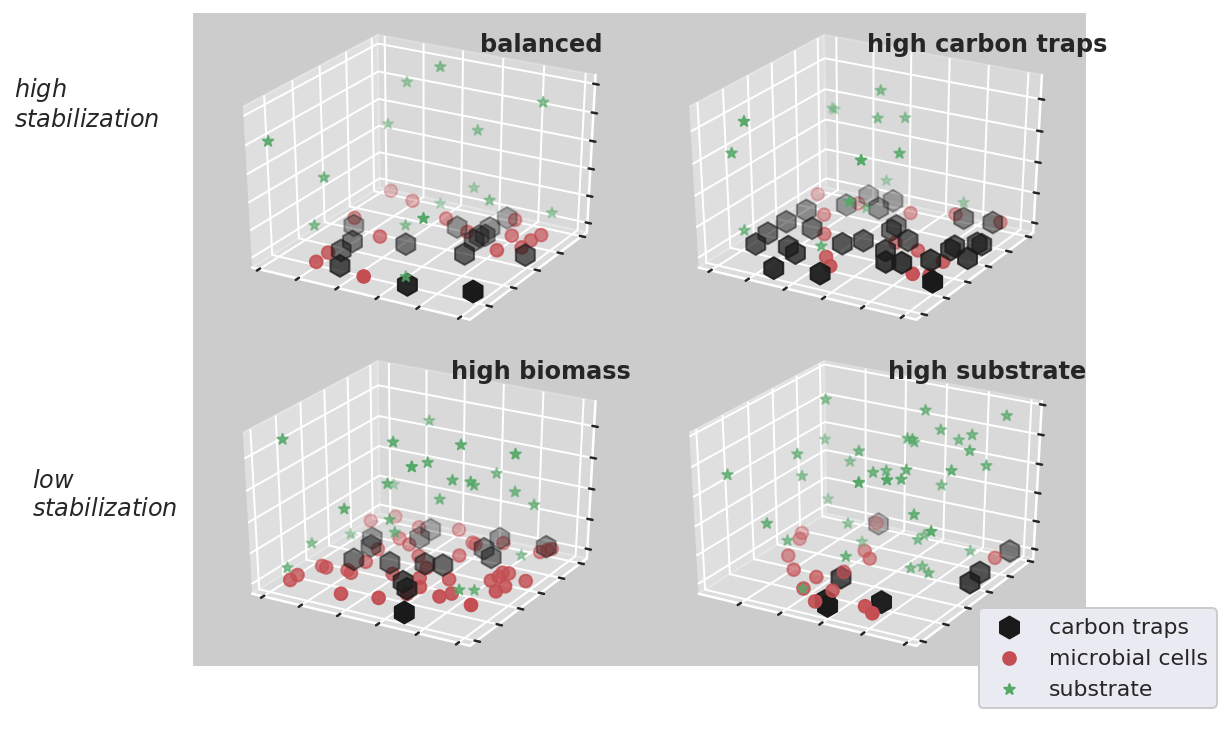
\includegraphics[scale=0.8]{thesis_figures/test/model_scenarios.png}
			\caption{examples of the different model scenarios with their corresponding outcome on the far left side of the figure}
			\label{fig:stabilization_model_scenarios}
		\end{figure}
		
		In the current experiment, a series of three consecutive, high rate applications of highly labile organic substrate was setup, each portion causing a rapid increase in microbial biomass followed by period of diminishing MB. In the first week for example, this strong microbial turnover likely yielded a large quantity of available carbonaceous organic substances in the form of necromass and other microbial products in the days following peak microbial growth
		(‘secondary pulse’),
		% microbial death
		and It is reasonable to assume that a substantial portion of this secondary pulse was still present in some sort of readily available form 7 days after MRE application (‘leftover carbon’), when a subsequent input was applied.
		% 	 \myRed{Substantial increases in net HWES during week 1 and 2 seem to correspond with such 'leftover carbon'}.
		Evidently, in all three LTTs, also the live microbial biomass as well as  aggregate structure had changed considerably between one MRE application and the next, particularly in the first and second weeks of incubation.\\
		Examined in light of the proposed stabilization model, these changes imply a modified setting into which MRE is applied in the 2nd and 3rd week. the large amount of labile carbon applied at $ T_0 $ had caused a surge of microbial growth (model variable (1)) which as suggested above, consequently resulted in a secondary pulse of large quantities of readily available microbial products (model variable (2)) yet proposedly, these pulses were not accompanied by proportional increases in potential sites of OM stabilization(variable (3)). considering the soil system right after the 2nd MRE application it is suggested that the sum of leftover carbon from the first application, along with newly introduced MRE carbon, resulted in a situation corresponding to scenario (1) in the stabilization model,  in which a high substrate-to-biomass ratio but especially high proportion of substrate to available stabilization sites would result in lower \gls{cue}.
		Direct meaningful  assessment of \gls{om} stabilization was not possible using data from the current experiment,
		it is assumed therefore that my \gls{cue} results provide a viable indication of the efficiency of short term \gls{om} stabilization (i.e the fraction of substrate-C remaining in the soil).\\
		%			 microbial products and necromass as primary source of stable \gls{som}
		microbial growth and respiration data in the 1st incubation week, seems to be in full agreement with the above proposed mechanism for reduced \gls{cue}. all three LTTs had seen a considerable increase in the weekly cumulative respiration while simultaneously presenting a notable decrease in the weekly microbial growth. the proportion of weekly respired $ CO_2 $-$ C $ to the weekly MRE-C applied had increased by roughly 10\% between the 1st and 2nd week while this same proportion for weekly microbial growth, decreased by more than tenfold for ORG and UNC and by a little more than half for MIN. given the validty of assumptions \ref{item: complete_uptake} and \ref{item: negligible_priming} of complete uptake and neglible priming, the inefficient use of MRE input in the 2nd, compared with the 1st week becomes evident. \\
		%	 \myRed{how exactly is the efficiency of microbial growth related to the efficiency of carbon stabilization, i.e \%stabilization?}\\
		according to the suggested 'stabilization model', higher substrate-to-biomass and a higher proportion of these two features to the availability of stabilization sites (or 'carbon traps'), would results in a smaller fraction of substrate-C remaining in the soil matrix, not necessarily less MBC being accumulated (as was observed in my results). however, it is suggested here that, besides ensuring carbon stabilization efficiency, a balanced proportion of available substrate, microbial biomass and soil pore availability for carbon protection, will also be reflected in more efficient accumulation of MB which would presumably result in a higher \%stabilization.\\
		%todo why higher biomass accumulation results in higher stabilization
		another soil feature that presented a strong reaction to consecutive MRE additions was the WEOC fraction. large pulses of WEOC were observed after each MRE addition (for the first week mainly in UNC) and these pulses increased considerably ( particularly for UNC and MIN) with consecutive additions. likewise the extent of these pulses was positively correlated with lower respiration rate and lower biomass among the three LTTs. this clearly points out to a phenomena mentioned earlier, whereby reduced microbial activity is reflected in greater accumulation of labile organic carbon, at least in the short term of a couple of days. in the 2nd week these trends in WEOC coincide with greatly reduced \gls{cue} in all three LTTs, and especialy in UNC, which incidently also had the highest WEOC accumaltion 24 h after MRE addition on that week. it seems that, mainly for UNC and MIN, the surge of easily available organic substrate ( from both 'leftover carbon' as well as from newly introduced MRE) has caused the microbial biomass to be overwhelmed, considerably reducing the uptake and utilization rate of available substrate in the first day or two after MRE addition and concurently also resulting in reduced weekly \gls{cue}.
		This was not the case for ORG, as the clear reduction in \gls{cue} was not accompanied by substantial pulses of WEOC.
		
		\section{Short term dynamics of \gls{som} pools in amended soils}
		%todo rephrase above title
		%todo rewrite opening section. shorter recap of the previuos section and include the opening of next subsection
		
		In this work, I’ve attributed particular importance to the proportion of Microbial growth to microbial respiration, expressed as the \gls{cue} index, as it was postulated to reflect to a large degree, the efficiency of incoming \gls{om} stabilization and incorporation into \gls{som}. This approach has proven to be at least partially successful in illustrating the effect of sequential labile substrate applications, as it indicated a reduction in \gls{cue} with each subsequent MRE addition. A much more limited success was achieved in trying to distinguish the effect of management history on the short term dynamics of \gls{som} pools, using  the \gls{cue} index. As noted earlier, ORG and MIN displayed a very similar  reduction in \gls{cue} throughout the incubation, while a somewhat erratic pattern was observed for UNC. Additionally, large uncertainties are associated with the weekly \gls{cue} results making it hard to assert  meaningful distinction between LTTs.\\ \pdfmargincomment[height=40pt]{I meant this opening section to lead to the fact that other parameters (like WEOC and HWES) revealed the effect of management history as opposed to CUE...}
		
		\subsection{Variability in WEOC removal}
		The dynamics of MBC by itself, also did not seem to reveal any significant differences between LTTs in their response to MRE input.
		However, the dynamics of CO2-Resp and moreover those of WEOC, in MRE amended samples, suggest a notable effect of management history on \gls{som} dynamics in this short term incubation. WEOC levels had peaked at almost 1000 mg/kg  24 h after the first MRE addition in UNC samples and the corresponding peak 24 h after the third MRE application in these UNC samples was almost double the size of the first peak. Data is missing for the second peak in UNC samples, yet it is assumed to have followed the trend suggested by the large differences between the first and third WEOC peak. This trend is similarly observed in MIN samples, albeit with a significantly lower intensity. Remarkably, these sharp increases in WEOC 24 h after MRE addition, were not observed in ORG on any sampling event.\\
		The intensity of WEOC pulses after each MRE addition increased both in time ( with consecutive MRE applications) and also between LTTs, in the following order, UNC $ > $ MIN $ > $ ORG. This order of response intensity between the three LTTs, most clearly notable 1 day after MRE additions, seems to be largely opposite to the order of baseline SOC content and baseline MBC between these LTTs, which were as follows, ORG $ > $ MIN $ > $ UNC (differences in MBC between ORG and MIN and between MIN and UNC in SOC, are not significant). This suggest  that higher initial \gls{som} content and/or higher extant microbial biomass may have been related to moderated fluctuations in WEOC following MRE additions and to moderated increases in the intensity of these fluctuations as the incubation preceded. \\
		Results from the preliminary incubation are indicative of the important role of microbial respiration in the removal of WEOC from the soil. Both Str or KWC amended soils as well as non-amended samples from the preliminary incubation presented an inverse trend between WEOC and Resp dynamics. However, no significant difference between ORG and MIN (in Str or KWC amended soils) was observed in terms of the efficiency of WEOC removal. In the MRE incubation, a comparison of WEOC dynamics with those of Resp revealed an opposite trend in the order of LTTs throughout most of the incubation. In this way soil samples in which Resp was high presented low WEOC pulses and vice versa. Although the sample size of different LTTs was quite low (N=3), the relation between microbial activity (Resp) and WEOC removal seems apparent. \\
		%	additionally, cumulative respiration in the three LTTs suggests the connection between elevated microbial activity (i.e respiration) and the quick removal of labile organic carbon.
		
		In the current experiment, an exceptionally high load of labile organics was applied with each MRE addition, roughly an order of magnitude higher than baseline MBC values.  Although labile DOM is usually rapidly consumed by the soil microbial population\myRed{*} it is possible that in situations were a proportionally large amount of labile substrate is rapidly introduced, the microbial population would be unable to process it completely\myRed{*} in the very short term of several hours to a day or two, and thus considerable amounts of substrate could be accumulated as WEOM. This seems to have been the case in the current experiment, where in the first week of incubation both ORG and MIN, presumably possessing a significantly higher reserve of active and potentially active microbial biomass, presented a very low increase in WEOC 24 h after MRE addition . This is suggestive of the metabolic capacity of these soil microbial populations allowing them to rapidly consume and break down the input substrate to the extent that it is unrecoverable as WEOM, either by mineralization of the substrate into CO2, its immobilization as MB or its transformation into metabolic products that would have been bound to the solid soil phase.
		%, rendering it unextractable with water.
		In the subsequent MRE additions, it is assumed that-although MRE input load was unchanged-the conditions with regard to microbial biomass and overall labile \gls{om} availability had been altered significantly, resulting in the increased intensity of WEOC pulses in these subsequent MRE additions (in MIN and UNC). As discussed in a previous section, it is suggested that by the end of the first week of incubation, the levels of labile \gls{om} availability had increased substantially (\textit{leftover carbon}). While MBC also increased  considerably in all three LTTs during the first week, it is proposed that the substrate-to-biomass  ratio had increased considerably between the first and second MRE additions in MIN and UNC, which may have been the primary reason for the observed pulses of WEOC following MRE addition, as the microbial populations in these soil samples were ineffective in removing the large influx of DOM during the first 24 h.
		
		In line with the proposed \textit{stabilization model} as well as the evidence presented earlier regarding the nature of DOM, I propose three  major drivers which controlled the dynamics of WEOC in the days following each MRE addition, each one represented by a measured soil feature:
		\begin{enumerate}
			\item microbial assimilation (MBC)
			\item microbial mineralization (CO2-Resp)
			\item potential for \gls{om} stabilization (AS, expressing the potential availability of the soil mineral phase for interaction with incoming decomposition products).
		\end{enumerate}
		
		
		while  CO2 mineralization can explain some of the variation in WEOC between LTTs, it is clearly not enough to explain all of the variation, as evident when comparing cumulative Resp trends with those of WEOC. The largest difference by far between LTT's in the percent change of cumulative respiration, is observed during the first pulse while subsequent pulses presented a much smaller and relatively minor difference between LTTs in terms of percent change in cumulative respiration.
		Microbial assimilation might have accounted for some of the variation yet no significant differences between LTT's were observed during the incubation.
		It seems therefore, that neither microbial growth (anabolism) nor microbial respiration (catabolism) can fully account for the variation between LTTs. The third driver listed above, namely soil potential for \gls{om} stabilization, remains thus as a possible candidate to account for the primary share of this observed variability. It is noted here that my analysis of soil aggregate stability provides only inferential information regarding the dynamics of soil stabilization potential, both due the low sampling frequency during the incubation as well as the nature of the test itself which provides a general indication of the aggregation status of the soil rather than a more detailed characterization of soil spatial organization. For example, an elaborate description of soil pore architecture including for example, pore size distribution and connectivity, could have been much more effective in examining the relation between stabilization potential and microbial efficiency in general and the short term removal of labile \gls{om} from soil solution in particular. \\
		Despite these limitations, AS is nonetheless presumed to provide valuable indications of a soil stabilization potential. The significantly lower \%WSA in UNC compared with the two other LTTs, throughout the incubation, is in accordance with the higher intensity of WEOC pulses in that LTT, suggesting structural features may have been a significant factor in this regard. However, differences between ORG and MIN did not correspond with the variations between these LTTs in terms of WEOC dynamics.  \\
		
		%\section{conclusions \hiddenTxt{limitations of the experimental setup}and suggestions for further research}
		%
		%		This research examined the effect of long term soil management and particularly fertilization management, on \gls{som} pools and related soil features such as AS. Our analysis of the dynamics as well baseline values of non-amended samples, provided strong evidence for the effect of 5 years of contrasting fertilization schemes on \gls{som} pools. These results indicated a clear distinction between organically and mineraly fertilized soil in both total SOC as well as biological \gls{som} pools. That this distinction was observed in soil samples obtained after a substantial resting period (\textit{no input + fallow}) in the original long-term experiment (GOP) is of particular interest.      , results from our MRE as well as Str and KWC amended samples were far more ambiguous.
		
		%The dynamics of WEOC in MRE amended samples present a definite distinction between LTTs, and this distinction matches clearly, though inversely, the variation between LTTs in baseline MBC and Resp. This \myRed{seemingly} negative correlation between WEOC on the one hand and extant microbial biomass on the other hand, similarly observed in all of the incubations during this research, provides strong evidence of the close association of microbial activity and WEOC. It is highly likely then, that increased microbial biomass and particularly active microbial biomass (as reflected in Resp) in the cultivated LTTs as opposed to UNC, had an essential role in driving this differential response between LTTS. This was corroborated to \gls{som}e extent by Resp dynamics during the MRE incubation itself, though not so much by MBC. The fact that microbial respiration is more strongly indicative of the active share of microbial biomass has been discussed earlier in this work. It is therefore not unlikely that the differential response of microbial biomass in terms of removal of WEOC for example, was not significantly reflected in MBC data.
		
		%preliminary incubation
		%	all treatment combinations presented a significant increase in WEOC on the first sampling event which was shortly after followed by a steep decline. the initial increase in WEOC was likely the result of substrate solubilization by water addition and/or microbial action, producing substantial amounts of WEOC. this easily available carbon pool was rapidly and continuously removed in the following days by microbial consumption, resulting in decreased WEOC. this decrease closely coincides with the time frame of maximum respiration, between 0-48 h, after which respiration rates had mostly leveled off. concurrence of WEOC removal with increased Resp levels, also observed for control samples in the preliminary experiment, effectively illustrates the  notion of WEOC as an immediate and labile source of energy for micro-organisms.
		
		
		The dynamics of HWES had also presented considerable variation between LTTs during the 28 days MRE incubation. The hot water extractable fraction of \gls{som} is often associated with aggregation processes, particularly its carbohydrate portion.  However HWEC and specifically HWES are also regarded as a labile source of energy utilized by the microbial population. In the current work, HWES dynamics during the MRE incubation mostly seemed to accord with the later view. When examining the net HWES accumulation in the course of the incubation, there appears to be a similar relation between HWES accumulation and the metabolic capacity of the soil (represented by MBC and moreover microbial Resp), as described above for WEOC. Although this relation is evidently not as clear as for WEOC, it does become more evident at day 21 and certainly at day 28 wherein the order of HWES content between LTTs is opposite with the general order of MBC and Resp as observed throughout my experiments. Clearly the significantly higher net HWES in UNC at days 14, 21 and 28, compared with both cultivated LTTs, is indicative of the lower metabolic capacity of this soil, as was also observed for WEOC. Here again, it remains unclear whether and in what way, the variation in HWES consumption and removal from DOM fraction is connected with microbial \gls{cue} and the carbon stabilization potential. However it appears that microbial capacity for labile carbon removal from DOM fraction is at least to some extent positively related with \gls{cue}, as evident from the inverse general trend in \gls{cue} as opposed to WEOC and HWES across the incubation period.
		

	\chapter{Conclusions}
		% !TeX root = ../main.tex
		
		% questions for Asher
		% 1. references for the idea that variabilty is inherntly greater in biologicL rather than chemical or physical tests.
		%todo TOC/SOC, our/my, we/I
		
		
		%\section{Preliminary incubation}
		
		\section{effect of management history on \gls{som} pools in non-amended soils}
		
		\subsection{Cultivated compared with non-cultivated}
		%todo how to cite this 'Seven-years of productivity and potential fertility in organically managed...' (ask Asher)
		Despite my expectations, both cultivated LTTs and especially ORG had resulted in higher baseline values for most parameters, compared with the non-cultivated LTT. Although agricultural intensification and long term fertilization has been repeatedly shown to diminish overall soil health and cause a reduction in \gls{som}, compared with non-cultivated soils \citep{laurance2014, mganga2016, tilman2011}, there is some evidence pointing out that this is not necessarily the case for certain agricultural management scenarios, particularly in arid and semi-arid environments.  For example, \citet{trivedi2016}, in a meta analysis, found that in arid climates, cultivated soils had on average significantly higher values of SOC compared with unmanaged soils. Similarly, repeated analysis of a large data base from soils in the US great plains area, revealed that SOC loss due to cultivation was lowest in low rainfall areas ($ \sim $300 mm MAP)\citep{miller2004, burke1989}. \citet{paz-kagan2014} conducted a research that included soils from the Migda research farm (\~{}30 km from the Gilat Research Center, with similar climatic conditions and soil properties), and found no significant improvement in Soil Quality Index(SQI) (including soil parameters such as \gls{soc}, hydraulic conductivity and surface hardness) when transitioning between agricultural land use and a natural ecosystem management. \citet{garcia-orenes2010} found no significant decrease in soil health parameters (TOC, WEOC, MBC, basal respiration) compared with an adjacent abandoned field (some natural vegetation cover) in soils from SW Portugal, treated for one year by  a number of different agricultural practices, including tillage and herbicide use. Although these different treatments were each tested separately (e.g compare tilled soil to non-cultivated soil),as opposed to combined long-term treatments in the current work (e.g. compare conventional management to unmanaged soil ), and lasted for only one year, nonetheless, the outcome of this work, clearly support the notion that certain agricultural practices may not have a detrimental effect on overall soil health when compared with non-cultivated soils in a semi-arid climate context. indeed some practices - in the case García-Orenes’s work, the return of substantial amount of oat straw – can actually cause a significant improvement in soil health parameters, not just compared with a non-cultivated soil but also compared with a natural cover soil ( Mediterranean woodland ).\\
		My results provide additional evidence supporting a similar line of evidence. Five years of intense compost application ( $ 6 m^3*year^{-1} $ ) combined with an otherwise conventional management system (Org), increased TOC by almost 60\% over an adjacent uncultivated soil (UNC). Org had also resulted in increased baseline levels of \gls{som} pools such as MBC, WEOC  and HWES-C  as well as higher basal RESP and higher AS, compared with UNC. \\
		Evidence from a number of experiments and review analysis, suggest that the net energy influx into the soil ecosystem from plants, can act as a key factor determining the rate and direction of changes in \gls{som} pools  and AS, when comparing cultivated and non-cultivated soils. \\
		Net primary productivity (NPP) is the net solar energy accumulated by vegetation per unit area and unit time. it is an important proxy of ecosystem function and carbon sequestration capacity\citep{jackson2016}. High NPP levels are likely to increase, besides plant biomass, the allocation of plant carbon and nutrients as root deposits, thus enriching the soil with labile, easily stabilized \gls{om}.  \\
		\citeauthor{trivedi2016}, compared cultivated and non-cultivated soils in the four major climatic regions of the world, and found NPP to be higher for non-cultivated soils in temperate and tropical climates and oppositely lower for non-cultivated soils in arid ecosystems. concurrently these trends where in accordance with SOC trends in soils from these two types of ecosystems, indicating the connection between the build-up of \gls{som}  and ecosystem productivty. \citet{bhardwaj2011} presented direct evidence relating the improvement in soil quality indices to increased NPP, when examining a set of long-term intensively managed row crop systems in the upper Midwest part of the USA.\\
		Considering the marked differences in management inputs between the cultivated and non-cultivated LTTs in the Gilat Organic Plots(GOP), in the form of water, fertilization and seeding, it is very possible that substantial differences in NPP between these two management systems occurred in various periods, especially during the long dry summers typical in this area, in which little  if any significant plant growth is expected in non irrigated soils. \\
		In light of these evidences, it is possible that differences in NPP between the cultivated LTTs and the non-cultivated LTT used in the current experiment, may have been at least partly responsible for the observed differences in \gls{som} related properties.
		This supposition is further supported by field observations and fertility tests from the GOP, where significantly higher crop yields were observed in ORG compared with MIN in various time points \myRed{* (\textit{Seven-years of productivity and potential fertility in organically managed Mediterranean Vertisol and semi-arid Loess soils})}. Although data for the complete calculation of NPP is missing in this long-term experiment, it is conceivable that higher crop yields were also expressed as higher NPP, eventually resulting in increased SOC (and related properties) accrual, an outcome that was observed in the current experiment. The \myRed{\textit{Seven-years of productivity and potential}} also reported increased weed coverage in Org compared with Min. This may have been an additional factor contributing to increased organic matter input in these plots.\\
		The possible importance of NPP in controling long term \gls{som} dynamics in these LTTs is in accordance with the latest emerging concepts of \gls{som} formation and preservation (\textit{ soil continuum model} ) as these views emphasize the role of a continuous flux of labile organic substances into the soil as a key feature in sustaining high levels of \gls{som} \cite{kleber2010, lehmann2015}.
		
		\subsection{Organic vs. chemical long-term fertilization}
		%todo find references for high variability in biological systems
		I expected 5 years of organic fertilization to increase \gls{som} pools over mineral-only fertilization, and indeed baseline TOC, WEOC and HWES (and HWEC, as observed in preliminary experiment) were significantly higher in ORG. on the other hand, no significant difference was observed between these LTTs in baseline MBC, CO2-Resp (actually higher in MIN samples in preliminary incubation) or AS. This statistical insignificance might be explained by management decisions applied in the GOP in the two years preceding soil sampling for the current experiment. As mentioned before, a zero fertilization period of two years, of which one year was fallow, preceded soil sampling (‘no input + fallow' period). The discontinuation of fertilization inputs practically eliminated management differences between ORG and MIN in that period, and the fallow period is likely to have caused significant reductions in biological activity and aggregate structure \citep{redmile-gordon2020, golchin1994}. this two year period may well have resulted in a ‘blurring effect’, causing any possible differences in MBC and AS to be considerably reduced.
		Statistical insignificance in microbial parameters probably also reflects high variability in the results , while it is suggested that the insignificance of differences in AS may be more expressive of actual similarity between these LTTs with regards to this particular feature.
		%	 High variability of biological soil features such as MBC and respiration is well documented.
		It is therefore suggested that the effect of contrasting fertilization schemes on AS persisted throughout this fallow period and were thus significantly detectable \hiddenTxt{effect was significantly detectable?} in my tests while microbiological parameters tended to fade away more quickly and were therefore less evident.
		
		\subsection{Microbial features}
		The average CO2-Resp rate (15.51 \respunit) and respectively the cumulative CO2-Resp (204.4 \cumrespunit) in control samples across the three LTTs, were of similar range as values reported for similar soils under similar conditions. \citet{ribeiro2010} measured 142.5 \genericunit of CO$ _2 $-C respired during a 21 day incubation, from an organically managed soil in SW Portugal (sandy soil, 9.3 $ g * kg^{-1} $ SOC). \citet{rudrappa2006} measured the CO2 mineralization of a soil subjected to different long-term combinations of organic and mineral fertilization, and found a range of between 100-150 \genericunit of cumulative CO$ _2 $-C after 21 days of incubation.
		The order of cumulative Resp between LTTs was in accordance with baseline MBC levels, indicating the link between these two features. \\
		The total cumulative respiration in the preliminary incubation, standing at 127 and 154 mg/kg after 168 h of incubation seem to be on the higher end of the literature reported range of cumulative respiration after one week of incubation without amendment. \citet{ribeiro2010} reported 52 \cumrespunit after 8 days of incubation without amendment and \citet{kemmitt2008} had reported similar values. \\
		the mean MBC across all sampling events in the preliminary incubation was \~{}400 mg/kg in both LTTs. This value is relatively high compared with some of the results from arable soils \citep{jat2020, haynes1999,garcia-orenes2010}, yet it is important to consider that extensive variation is reported for MBC depending on various edaphic and climatic features as well as temporal variability. A comparison of the initial MBC value from my preliminary and main incubations demonstrate this kind of variability. Initial MBC in the non-amended samples from the main incubation stood at \~{}200 \genericunit while the level of MBC in these corresponding samples from the preliminary incubation did not decrease below 350 \genericunit. This distinction was probably related to the effect of rapid increases in humidity level (wetting of soil samples) on the microbial population and the different time frames captured by these two experiments, due to differing pre-incubation periods (detailed discussion follows shortly).\\
		Interestingly, control samples did not show a sharp pulse of microbial growth in the first 24 h of incubation, as was observed in the main incubation. In Min samples only a small insignificant increase was observed during the first 24h while for Org, a significant and considerable increase in MBC was observed after 48h, yet this was  not nearly as large as the increase observed in the main experiment. This contrast between the controls of the main and preliminary incubation was similarly observed for Resp and WEOC. Respiration in the preliminary incubation was higher than in the main incubation during the first 24 h, thereafter presenting comparable values. initial WEOC levels in the preliminary incubation were \~{}4 times higher than initial values in the main incubation control samples. This discrepancy may have been related to the different duration of pre-incubation in these two experiments ( 48 h vs. 120 h in the preliminary and main incubation respectively). It is suggested that the shorter pre-incubation in the preliminary experiment resulted in a different snapshot of the dynamics being captured by my sampling in these two experiments. Presumably the 5 day pre-incubation in the main incubation had initially caused an increase in microbial activity and WEOC which had - by day 5 when the actual incubation was initiated ($ T_0 $)-been mostly diminished. this pulse dynamics following a rapid increase in water content was repeatedly observed, to varying degrees, in the preliminary and main incubation following water additions and is furthermore commonly reported in literature (see discussion and relevant references in section \hyperref[subsection_4.2.2]{section 4.2.2}). this presumed decline in microbial activity and WEOC can explain the relatively low levels of these soil features at $ T_0 $ in the main incubation . Contrarily, it is most likely that a similar pulse of microbial activity and WEOC in the pre-incubation of the preliminary experiment, had not already seen a such considerable decline after only 48 h. Thus, the higher levels of microbial biomass and activity as well as WEOC at $ T_0 $ in controls samples in the preliminary incubation, supposedly express the different time frame being observed. The intense pulse of microbial growth observed in the main incubation (but not in the preliminary incubation) during the first 24 h supports the above explanation.\\
		% this should be it's own subsection
		baseline MBC levels for all three LTTs were in the range of published data regarding arable soils\citep{gonzalez-quinones2011}. \citet{rotbart2018} measured the seasonal dynamics of MBC in field samples from the same plots used in this work (UNC was not included in that work) and found a range of values mostly between 100-500 \genericunit over a period of more than 3 years (excluding the temporary effect of compost application). These result are similar to the baseline values reported here.
		in line with my expectations, the long-term organically fertilized LTT, had higher control values throughout most of the main incubation period, compared with the long-term minerally fertilized soil. yet these differences were almost all statistically insignificant. The calculated baseline value for MBC was 36\% higher in ORG compared with MIN (non-significant). it is not entirely surprising that the differences between control samples from ORG and MIN in this current experiment were statistically insignificant, considering that no statistical significance was found between these  two LTTs in the majority of 12 field samples taken over a period of more than two years in the work of \citet{rotbart2018}, particularly for sampling dates outside the immediate effect of fertilizer application.\\
		%			\myGreen{statistical insignificance may also be due to 'blurring 	effect' mentioned in the above section}\\
		Other works that had examined the effect of long-term fertilization on MBC in semi-arid soils, showed a definite effect of long-term fertilization management on the levels of MBC, with most results indicating an increase of MBC for organically fertilized soils compared with chemically fertilized soils\citep{luo2015, liu2013, ghoshal1995}. it should be noted though, that these above cited results are from experiments spanning considerably longer periods, possibly increasing the likelihood of obtaining clearer and more significant results.\\
		%			Why longer periods would provide clearer results… obvious?
		ORG and MIN both caused an apparent increase in MBC compared with UNC. This interesting result, discussed earlier in the general context of the effects of cultivation on \gls{som} pools, has little support in literature with regard to MBC levels. indeed many researches present an opposite trend in which long term transition from a non-cultivated, undisturbed soil management to an agriculturally managed system, usually causes a decrease in MBC levels along with decreases in \gls{som} stocks \citep{benbi2015, yu2013,zhou2018}. it is worth noting that many of the works that examined the effect of land use on MBC have been carried out in temperate and tropical climates, in areas where NPP is often considerably higher then in semi-arid and arid climates in the Mediterranean and similar regions.\\
		%			\myGreen{xpand on the fact most works that showed higher MBC in non-cultivated soil compared with arable soils are from temperate or tropical climates, where NPP is liable to be higher in unmanaged, non-cultivated soils. }
		%
		\subsection{WEOC}
		DOC is often correlated with SOC content and has been regarded as being in equilibrium with the solid phase \gls{som} \citep{malik2013}. In this work, the number of data points was not sufficient to produce meaningful statistical relationship between these two parameters. Nonetheless, the clear separation between Org and the two other LTTs in both SOC and WEOC suggest that a considerable association existed between these two parameters for non-amended samples in this incubation. Baseline SOC level seemed to correlate with WEOC (and with HWES which likely also implies a correlation with HWEC as it has been demonstrated that HWE total carbon and carbohydrates maintiand a costant ratio in non-amended samples).
		Baseline WEOC values were comparable to literature reported results from soils of similar SOC content. Evidence from Long term fertilization plots in central china, presented WEOC concentrations in the range of 25-55 \genericunit for NPK and pig manure fertilized plots respectively\citep{xu2018}. These values are a little lower than my calculated baseline values yet they compare very similarly to the initial WEOC levels that were measured (immediately after the first water addition, that is  at the end of a 5 days pre-incubation period at a constant 50\% WHC water content). \citet{hamkalo2014} reported similar values, with an average of \~{}40 \genericunit for the 0-15cm  soil layer in a manure and NPK fertilized soil (\~{}1.6\% SOC).
		the higher levels of WEOC in Org compared with Min, observed throughout the preliminary incubation, probably reflect higher SOC stocks in Org, as WEOC levels are often closely related to \gls{som} stocks\citep{malik2013} .\\
		In the preliminary incubation, WEOC dynamics seem to inversely correspond with both Resp dynamics and MBC dynamics. This is clearly manifested in Org samples, where a substantial MBC pulse between 24 and 96 h is concurrently accompanied by a decrease-increase pattern of very similar proportions in WEOC. There seems to be a certain delay before WEOC responded to changes in Resp rate, as peak Resp is observed in the first 24 h while WEOC begins to decline just after that time period. Nonetheless there is a considerable concurrence between these two parameters, as WEOC declines rapidly during a the 24 to 48 h period when Resp are still relatively high and inversely increases between 48 and 96h, when Resp rates had mostly reached their lowest level, showing little change in that time period. These concurrent dynamics may reflect the often noted interrelation between these three soil parameters. MBC and Resp are clearly closely related, yet it is also a common view that WEOC represents a labile DOM pool that serves as an easily available energy source for micro-organisms and is thus closely associated with the dynamics of microbial activity \citep{kemmitt2008, kaiser2012, guggenberger1998}. Results from the preliminary incubation, are in accordance with this line of evidence.\\
		
		
		\subsection{Hot water extractable organic matter fractions}
		%todo maybe rephrase this title
		HWEC and HWES presented very similar dynamics throughout the preliminary incubation, implying that HWES constitutes  a more or less constant fraction of HWEC under these particular conditions. Similar observations were made by \citet{haynes2005} and \citet{ghani2000, ghani2003} though both reported higher proportions of sugar-C in HWEC. It is likely that this higher ratio is related to higher \gls{om} content and the presence of annual grasses in the soils referred to in these works, as this type of land cover has been associated with higher sugar-C content in HW extracts \citep{haynes1993}.
		notably, HWEC and HWES dynamics were not as accordant with MBC and Resp dynamics as WEOC seemed to be, and likewise, their fluctuation during the preliminary incubation relative to initial values, were not as intense as in WEOC, which had seen a \~{}70\% decrease from its initial value(after 48 h). This may reflect the sizes of these HWE carbon pools in the current experiment, which were \~{}3 to \~{}10 times larger than WEOC in control samples (for HWEC and HWES-C respectively). Additionally, the HWEC pool is less susceptible tp microbial degradation than WEOC and  considered more stable. Thus, given any control of microbial action on the dynamics of HWEC (or HWES), it would probably have been less significant than for WEOC and these possible effects would have been far less noticeable due to the large proportion of HWE fractions in comparison with the size of microbial biomass, and the extent of its activity (e.g respiration rate). Indeed, the total cumulative respiration  for the preliminary incubation, in either Org or Min was less than 200 mg/kg CO2-C and the largest increase in MBC, recorded in Org samples between 24-48 h, was \~{}150 mg/kg. These possible pools would account for no more than 25 and 40\% of the initial HWEC in Org and Min respectively. \\
		these results support the view of WEOC as a dynamic organic matter pool, easily available for microbial consumption and highly affected by microbial activity. Concurrently, the apparent contrast between HWEC dynamics and those of WEOC, suggest that this pool is considerably more stable, and more moderately affected by microbial action.\\
		Interestingly, in the main incubation, Org samples had seen larger variations in HWEC compared with Min, particularly in the first 24h. This could not be straightforwardly linked with microbial parameters, as MB size or growth rate did present any distinction between the two LTTs during the first 24 h, and moreover, respiration rates were significantly higher in Min throughout the incubation and specifically during the first 24h. This would likely preclude the possibility of microbial consumption being responsible for this larger fluctuation in HWEC.\\
		Baseline HWES concentrations were similar to those reported by other works for agricultural soils \citep{haynes2005, yousefi2008, puget1998}. HWES are considered sensitive indicators of changes in soil quality\myRed{*}. In this work this parameter was able to significantly distinguish between the different long-term treatments.\\
		Similar to my results, both \citet{yousefi2008} and \citet{bottinelli2017} had found increased levels of HWES in organically, or organically combined with chemically fertilized soils compared with chemical-only fertilized soils.
		In the work of \citet{yousefi2008}, long-term (5 years) manure fertilized soils, in three rates of application  25, 50 and 100 $ Mg * ha^{-1} * yr^{-1}  $ , increased the concentration of HWES by roughly 20, 100 and 300 \genericunit compared with a chemically fertilized soil, respectively. The chemical fertilizer treatment, in that work also differed from the manure treatments in its crop rotation scheme, which included a fallow period between consecutive crops. The \~{}100 \genericunit increase in HWES observed in ORG compared with MIN in the current experiment, is comparable to the results presented by \citeauthor{yousefi2008} for the 50 Mg/ha manure treatment, which was similar to the 38 $ Mg * ha^{-1} * yr^{-1}  $ of compost applied annually in ORG.
		\citet{bottinelli2017}, compared soils treated for 7 years with either ammonium nitrate or poultry manure (manure was supplemented with mineral N to yield equivalent amounts of nitrogen), their results  showed a significant increase (\~{}100 \genericunit) in HWES for the poultry manure treatment compared with the mineral fertilizer-only treatment.
		Compared with the difference observed between ORG and MIN in this current work, which amounted to more than 30\% increase, the increase as a percent of the  chemically treated soil, presented by Bottinelli, was much smaller at 7\%. This was attributed to the low annual application rate of manure ( 17 $ Mg * ha^{-1} * yr^{-1}  $ ) as well as high initial HWES and \gls{om} content in that soil.
		
		\subsection{Ergosterol}
		the reduction in ergosterol in Org samples in the preliminary incubation, suggests a decline in fungal biomass, possibly through the effect of water addition as soil moisture has been shown to affect the abundance of fungal populations \citep{drenovsky2004, griffin1963}. the decline in Ergosterol as a \% of MBC suggest that fungal biomass was preferentially impaired as opposed to bacterial species, yet this observation can not be backed by statistical evidence, mainly due to the large errors associated with MBC data in the first 2 samplings.\\
		the Erg-to-MBC ratio, was the only parameter for which UNC had a significantly higher baseline value compared with the two other LTTs (roughly 50\% higher than baseline Erg-to-MBC value in ORG or MIN).
		ORG had a higher ratio than MIN, though this difference was not significant. The ERG-to-MBC reflects, with certain limitations, the ratio of fungal biomass to the total microbial biomass. Ergosterol does not represent arbuscular micorhyzal fungi (AMF), however, Since the experiments included in this work were performed without any living plants, it is reasonable to assume that the fraction of AMF and other plant symbiotic species, from the total funagl biomass is negligible.
		It is generally agreed that changes in land use will have significant effects on microbial community composition\myRed{*}. agricultural intensification, especially but not exclusively increased tillage, can cause a reduction in overall fungal biomass and consequently a reduction in the fungi-to-bacteria ratio\myRed{*} although some results showed no significant differences\myRed{*}.
		the current result, showing a significant reduction in ERG-to-MBC as a consequence of long-term cultivation practices, compared to a non-cultivated soil, is therefore mostly supported by prior evidences.
		studies have shown contrasting results regarding the effect of long-term organic or mineral fertilization on the ERG-to-MBC ratio. \citet{heinze2010} found an increase in ERG-to-MBC in long-term chemically, compared with organically, fertilized soils, yet the mineral treatment was accompanied by a high straw return while the organic treatment was not, indicating that these differences might not have been  singularly affected by synthetic nitrogen application. A recent work by \citet{knoblauch2017} also found significantly higher values of ERG-to-MBC in long-term chemically fertilized grasslands, compared to soil subjected to organic amendments in the form of cattle slurry. However, cattle slurry has been shown to increase bacterial over fungal biomass \citet{knoblauch2017}.
		\citet{probst2008} found a significant increase in ERG-to-MBC in organically managed vineyard soils receiving occasional compost doses, compared with conventionally managed soils receiving customary amounts of NPK. This extensive work included four pairs of organically and conventionally managed vineyards yet it is hard to determine the specific effect of the contrasting fertilization schemes since these were not separated from other variables such as tillage, certainly an important factor with potential influence. A more recent work by \citet{mackie2015} , also performed with vineyard soils, evaluated the effect of a one time compost application on ergosterol and found a significant increase after 6 months compared with a non-amended control soil. It is not entirely clear whether a similar effect was found for the ERG-to-MBC ratio since these results were not reported explicitly and it is was not possible to establish them from the provided data.
		Given the unresolved nature of these evidences, it is not surprising that no significant difference in the ERG-to-MBC ratio was observed between ORG and MIN in this current work. However a clear distinction was observed between the two cultivated soils and UNC suggesting that factors other than fertilization, such as tillage, irrigation and plant productivity might have had a more substantial effect on the proportion of fungal biomass to the total microbial biomass.
		the Erg-to-MBC ratio, was the only parameter for which UNC had a significantly higher baseline value compared with the two other LTTs (roughly 50\% higher than baseline Erg-to-MBC value in ORG or MIN).
		ORG had a higher ratio than MIN, though this difference was not significant. The ERG-to-MBC reflects, with certain limitations, the ratio of fungal biomass to the total microbial biomass. Ergosterol does not represent arbuscular micorhyzal fungi (AMF), however, Since the experiments included in this work were performed without any living plants, it is reasonable to assume that the fraction of AMF and other plant symbiotic species, from the total funagl biomass is negligible.
		It is generally agreed that changes in land use will have significant effects on microbial community composition\myRed{*}. agricultural intensification, especially but not exclusively increased tillage, can cause a reduction in overall fungal biomass and consequently a reduction in the fungi-to-bacteria ratio\myRed{*} although some results showed no significant differences\myRed{*}.
		the current result, showing a significant reduction in ERG-to-MBC as a consequence of long-term cultivation practices, compared to a non-cultivated soil, is therefore mostly supported by prior evidences.
		studies have shown contrasting results regarding the effect of long-term organic or mineral fertilization on the ERG-to-MBC ratio. \citet{heinze2010} found an increase in ERG-to-MBC in long-term chemically, compared with organically, fertilized soils, yet the mineral treatment was accompanied by a high straw return while the organic treatment was not, indicating that these differences might not have been  singularly affected by synthetic nitrogen application. A recent work by \citet{knoblauch2017} also found significantly higher values of ERG-to-MBC in long-term chemically fertilized grasslands, compared to soil subjected to organic amendments in the form of cattle slurry. However, cattle slurry has been shown to increase bacterial over fungal biomass \citet{knoblauch2017}.
		\citet{probst2008} found a significant increase in ERG-to-MBC in organically managed vineyard soils receiving occasional compost doses, compared with conventionally managed soils receiving customary amounts of NPK. This extensive work included four pairs of organically and conventionally managed vineyards yet it is hard to determine the specific effect of the contrasting fertilization schemes since these were not separated from other variables such as tillage, certainly an important factor with potential influence. A more recent work by \citet{mackie2015} , also performed with vineyard soils, evaluated the effect of a one time compost application on ergosterol and found a significant increase after 6 months compared with a non-amended control soil. It is not entirely clear whether a similar effect was found for the ERG-to-MBC ratio since these results were not reported explicitly and it is was not possible to establish them from the provided data.
		Given the unresolved nature of these evidences, it is not surprising that no significant difference in the ERG-to-MBC ratio was observed between ORG and MIN in this current work. However a clear distinction was observed between the two cultivated soils and UNC suggesting that factors other than fertilization, such as tillage, irrigation and plant productivity might have had a more substantial effect on the proportion of fungal biomass to the total microbial biomass.
		
		\subsection{Aggregate Stability}
		A significantly higher baseline AS was observed for the cultivated LTTs in my experiment. This is in line with the other results reported here, showing a clear advantage for agricultural management (particularly when combined with compost fertilization) compared with non-cultivated soil in this specific context, with regard to increasing \gls{som} stocks and enhancing related soil properties (such as biological activity, i.e MBC and respiration). Long term fertilization treatments (ORG and MIN), on the other hand, could not be statistically separated based on AS values. ORG had a higher AS baseline value than MIN, yet this difference was not significant, possibly due to the \textit{blurring effect} mentioned earlier. \\
		\citep{golchin1994} proposed a mechanism for organic matter input decomposition, suggesting that the formation and persistence of soil aggregate depends on the continuous input of organic matter into the soil. In line with this mechanism, the works of \citep{li2007} and \citep{redmile-gordon2020} provided evidence from field experiments showing a decrease in both SOC and aggregate stability during both long and short term periods of reduced or eliminated organic input.\\
		Results from the current work support this kind of evidence, showing  a marked decrease in AS in non-amended samples (Control) during a one month incubation ,compared with significant increases in AS when organic substrate (MRE) has been applied.
		Whatever significant differences in AS that might have been observed between ORG and MIN during the early period after LTTs were  effectively ceased (begining of the \textit{no input plus fallow period} ), it is \myRed{very} possible that these differences had been considerably diminished by the end of this two year period.\\
		
		\subsection{Short term dynamics of \gls{som} pools in non amended samples}\hypertarget{subsection_4.2.2}{}
		
		large increases in respiration rate were observed following each water addition. it is likely that these respiration pulses were due to the effect of water additions, considering the tight temporal proximity between these events. the first water addition was followed by a sharp increase in MBC and WEOC (roughly an order of magnitude increase between $ T_0 $ and $ T_{24h} $). while subsequent water additions were also followed by significant increases in MBC, these were much smaller and they diminished considerably between the 2nd and 3rd water addition. for WEOC there seemed to be no apparent response to the 2nd and 3rd water additions.
		studies have reported substantial increases in microbial activity (biomass and respiration) as well as in DOM\citep{fierer2003}, also accompanied by decreases in aggregate stability measures\citep{cosentino2006}, after a drying-wetting cycle, as opposed to constant water content. These phenomenon are sometimes referred to as the ‘birch effect’.  My results are in line with these evidences, as significant increases (for all LTTs) in  $CO_2 $, MBC and WEOC  were observed in the 24 hours following the first wetting event as well as a significant decrease in AS during the first half of the incubation (and similarly during the second half, except for ORG). Although the current experiment did not include a typical drying-wetting cycle as common in  studies on the subject, including those cited above, my soil samples did experience a period of air dry conditions (3-4 months in the field  and then another 1-3 months in air tight bags at 4C) followed by wetting to moderate water content for 5 days(50\% WHC during pre-incubation) and then another wetting event at the onset of the incubation. It is therefore suggested that the observed changes following the second wetting event, i.e at $ T_0$, begining of incubation, were of similar essence as those described in the above mentioned studies, as this type of soil response has also been observed following a rapid increase in water content even when the soil was already in wet conditions\citep{xiang2008, rey2005}.
		enhanced microbial activity following increases in water content can be relalted to a number of different underlying causes, among them the release of \gls{som} into available forms, due to either aggregate disruption caused by slacking,  or desorption and redistribution effects due to water flow inside soil pores \citep{xiang2008}. the later mechanism was explained by \citeauthor{xiang2008} as being the result of diffusion limited \gls{om}, being protected from microbial attack under constant water content and subsequently made available upon rewetting by the flow of water causing desorption and redistribution of this material. \\
		%\myGreen{why later water additions did not result in substantial increases in MBC and no increase in WEOC?}\\
		WEOC levels had seen a sharp increase in the 24 h following the first wetting event followed by relatively steady concentrations in the next few days and then a sharp decrease following the next wetting event.
		These  dynamics and the dynamics of microbial activity (MBC and CO2-Resp) could be explained by a cascade of processes driven by the the first wetting event. These processes involve the physical action of water addition and the biological action of micro-organisms, both acting simultaneously as a possible enhancing agent as well as a possible sink for DOM. It is possible that the rapid increase in WEOC observed during the first 24 h, was the result of water addition causing desorption and redistribution of available \gls{om}, thus increasing WEOC levels. These increasing WEOC levels may have been used by micro-organisms to fuel the observed growth burst during the first 24 hours, possibly causing further enhancement of DOM replenishment.  A period of relatively steady WEOC concentrations as well as respiration rates then follows until day 7 or 8 (depending on LTT), from which time WEOC concentrations fell sharply, especially in the lower SOC LTTs, MIN and UNC.
		One possible explanation for this sharp decrease in WEOC content could be enhanced microbial activity, rapidly consuming any available DOM (and thus increasing the diffusion potential for \gls{som} solubilization), combined with a simultaneous decline in the availability of solid phase \gls{som} for desorption and solubilization, ultimately limiting the supply of additional \gls{om} into the dissolved pool.
		%		It is possible that during the first week of incubation, desorption by wetting effect combined with increased solubilization by the enhanced microbial population, had reduced substantially the \gls{som} constituents  most readily available for desorption or microbial solubilization by extracellular enzyms \myRed{*}. \\
		The dynamics of AS concur with this kind of explanation. A significant and clear reduction of AS in control samples was particularly evident in MIN and UNC, both sustaining considerably lower SOC levels compared with ORG. It is suggested that the higher SOC stocks in ORG, producing higher concentrations of labile WEOC that could sustain microbial activity throughout the incubation period , was thus able to ensure continued aggregate formation and buildup. Contrarily, in the two other LTTs, where initial SOC stocks were considerably lower, it is suggested that microbial activity had exhausted most of the easily available WEOC, possibly inducing the microbial population to direct their efforts for energy extraction to other carbon sources such as those involved in stabilizing soil aggregates. This could explain the more drastic reduction in AS observed in UNC and MIN and furthermore supports the notion that maintained aggregate stability requires some degree of continues inflow of easily available organic matter \citep{golchin1994}. \citet{cook1992} had observed a decreased microbial utilization of DOC after two weeks of incubation despite high contents of DOC, suggesting the preferential accumulation of recalcitrant DOC.\\
		HWES are often regarded as a potentially biologically available \gls{om} pool which also has an important role as an aggregation agent. Nevertheless, only a slight reduction in HWES concentration was observed during the incubation, and this was in the first week of incubation. It seems therefore, that AS decline could not be primarily attributed to the degradation of HWES. Since total HWE carbon data is not available for this incubation, it remains unknown whether the degradation of other HWE components may have been related to AS decline and whether this degradation was indeed initiated by  the exhaustion of easily available carbon fraction such as WEOC.\\
		%		\myGreen{here: literature supporting the above mechanisim}  \citet{cook1992}\\
		\hypertarget{weoc_decrease}{}
		Contrasting dynamics between ORG and the two other LTTS was also observed for WEOC. The decrease in WEOC levels in ORG was delayed compared with the two other LTTs as it started on the 8th and not the 7th day of incubation, and was furthermore significantly smaller, as WEOC dropped by \~{}40mg/kg compared with the \~{}80 mg/kg drop observed for MIN and UNC. This delayed and limited decrease can be attributed to the higher \gls{som} stocks in ORG which might have allowed the solid phase \gls{som} to continue in sustaining relatively high WEOC concentrations despite increased solubilization of \gls{som} through microbial action and possibly increased water content effect.\\
		The above explanation (‘DOM first’ rational) implies  the reduction in microbial activity is largely driven by decreased substrate availability, as easily degradable DOM supply was supposedly significantly reduced during the first week of incubation. The relatively concurrent variations in WEOC and CO2-Resp seems to be in agreement with this kind of description, particularly for UNC and MIN LTTs, in which CO2-Resp dynamics between days 7-10 (excluding the first few hours after the 2nd and 3rd water additions) appear to follow the dynamics of WEOC, albeit with a delay of 24 hour. some  degree of discordance with this reasoning is expressed in MBC dynamics, as the decrease in its concentration preceded that of WEOC and  CO2-Resp by several days, which might suggest an alternative explanation for their subsequent decline, namely that a considerable reduction in microbial activity and the consequent decrease in \gls{som} solubilization, was the primary driver for the observed decline in WEOC ( ‘microbial activity first’ rational) as opposed to DOM levels dictating the degree of microbial activity as suggested in the \textit{DOM first} rationalization.\\
		It is a common view, that only a certain fraction of the total MB  is involved in the important processes of biogeochemical transformations in the soil \citep{blagodatskaya2013, salazar-villegas2016} and that this fraction is much more accurately reflected in microbial respiration values than it is in total microbial biomass (TMB) estimations (e.g. MBC)\citep{salazar-villegas2016}. It is therefore suggested that although MBC levels started to decline several days before any decrease in WEOC was observed, this does not necessarily imply a causational relationship. Considering the high level of CO2 production rates during the first week of incubation, even when MBC had declined significantly, it is suggested that an active fraction of the TMB had kept microbial activity levels, particularly with regard to \gls{som} decomposition, at relatively constant intensity, despite the large die off in the overall population. \\
		
		
		\subsubsection{Ergosterol}
		
		except for a single sampling event (KWC amended MIN samples at 24h) none of the four treatment combinations had shown any significant difference in the \% Erg from MBC, compared with their respective control samples. this is regardless of the sharp increase in Erg concentrations in STR amended samples. for these STR amended samples, it seems that any increase in Erg was accompanied by an equivalent increase in bacterial biomass, which precluded any significant changes in the Erg-to-MBC ratio. for KWC amended samples, both the overall biomass as well as the Erg concentration remained relatively constant throughout the incubation. \\
		
		
		\section{Effect of consecutive MRE additions}
		Apart from studying the effect of long-term management history on \gls{som} pools, I set out to examine the effect of consecutive applications of labile organic substrate on the short term dynamics of different \gls{som} pools (research objective \#3). In particular, I wanted to see how this sequential introduction of high load labile substrate will effect microbial substrate use efficiency.\\
		This section examines the results from MRE amended soil samples, specifically relating them to the effect of the short term treatment and setting the discussion of long term management history effects to a later section. Thus any reference to the results or trends that appear in this section is relevant to all three LTTs unless otherwise mentioned.\\
		All three LTTs were strongly affected by MRE additions as evident from the high microbial activity ( MBC growth, CO2-Resp) that was measured 24h after each MRE addition (peak MBC after the 2nd MRE addition is \myRed{extrapolated} \hiddenTxt{maybe assumed?}). This sharp microbial growth during the first 24h was then followed by a somewhat similarly sharp decrease  in the next two days and a steadying of MBC up to day 7 when a new input was applied. This pulse of microbial growth and respiration is a common phenomenon for labile substrate decomposition in soils.
		Strong microbial activity was  observed by various other works shortly after applying either glucose or mixtures of labile organic substances (e.g MRE) as a substrate \citep{hill2008, landi2006, traore2000}.
		This strong treatment effect was expected since MRE application rates used in this experiment were considerably high, representing at least 10\% of SOC depending on LTT. These rates were also high compared with most estimates of the average flux of exudates secreted by plant roots. Early works, focusing on the single root scale, have estimated the total rhizodeposition flux to be in the range of 50-100 $ \mu g * g\ soil^{-1} * day^{-1} $, roughly 3 times lower than the rate used in my experiment. A more recent work by \citet{pausch2018}, aimed at evaluating rhizodeposition rate at the field scale, had predicted even lower rates. These disagreements express the inherent difficulties in obtaining realistic assessments of rhizodeposition fluxes, resulting from both methodological limitations and the intrinsically variable nature of this flux, which can change rapidly in magnitude depending  on the complex interactions between the plant and its environment.
		
		\subsection{Reduced weekly \gls{cue} following consecutive MRE additions}
		
		A clear reduction in the weekly microbial growth was observed for all three LTTs during the 2nd and 3rd weeks, compared with the 1st week of incubation.
		Weekly cumulative Resp on the other hand, had increased considerably between the 1st and 2nd weeks, while decreasing once more between week 2 and 3.
		the use of these microbiological features to calculate the weekly \gls{cue}, presented a clear pattern for ORG and MIN, whereby the weekly \gls{cue} was substantially reduced following the 2nd MRE addition (by roughly 50\%) and remained similarly low in the 3rd week (\gls{cue} was not calculated for the 4th week since respiration data was not available. for UNC the trend in weekly \gls{cue} was rather less obvious.\\
		\myRed{As noted earlier/as noted in Materials and Methods chapter}, the appropriate derivation of \gls{cue} from unlabelled data requires the satisfaction of two assumptions regarding the relevant time frame:
		\begin{enumerate}
			\item \label{item: complete_uptake}\textbf{complete uptake} - that the large majority of input-C had undergone microbial uptake.
			\item \label{item: negligible_priming}\textbf{negligible priming} - that the proportion of primed carbon inside newly formed MB or its share in the total respired $ CO_2 $, is negligible.
		\end{enumerate}
		Assumption (1) can be partly justified, at least regarding the first week, by  my own results,  observing the fact that peak net MBC (peak growth) for that week stood at \~{}2000 \genericunit for all three soils, similar to the 2200 \genericunit of MRE input-C applied at $ T_0 $. this implies that most of the  input-C had been used for microbial growth 24h after the 1st MRE application. Evidently, at least some of this MBC had originated from \gls{som} or from existing MBC (priming effect), hence the satisfaction of assumption (2) is valuable for supporting assumption (1). regardless of the origin of the carbon observed as peak growth, a  number of studies had shown glucose-C inputs of varying intensities to be completely decomposed after 2-3 days of incubation by the most\citep{hill2008, landi2006}, further supporting the notion that little if any input-C could have been recovered untransformed by the end of the 1st or for the matter also the 2nd and 3rd week.
		regarding the priming of existing MB (assumption 2), it should be noted that the high t peak growth observed in all three LTTs for the first week, far exceeds the initial MBC, indicating a low contribution for this component at least in the first week.
		As to the \gls{som} derived C as a substantial source of MBC growth and/or CO2 efflux during each of the 1st 3 weeks of incubation ( assumption 2),  support for its relatively small contribution in this particular situation is given by a number of recent experiments demonstrating the negative correlation between substrate-C load and the magnitude of priming effect\citep{blagodatskaya2011, schneckenberger2008, wu1993}.
		given the above considerations, it is assumed that the specific utilization of the \gls{cue} index in the current work, is justified and reasonable.\\
		Evidently, the specific application of \gls{cue} in this work and particularly it's application on a weekly basis, limits the resolution by which the controls of \gls{cue} can be discerned. Regardless, at least for ORG and MIN, these \gls{cue} trends clearly indicate that the consecutive additions of a large pulse of highly labile organic substrate resulted in a considerable reduction in the overall soil efficiency of substrate utilization. Consequently this reduced \gls{cue} implies a reduced carbon stabilization as \gls{som}, to the extent that efficient micorbial growth is translated to increased carbon stabilization.
		
		\vspace{\textheight }
		\subsection{A conceptual framework for the decomposition and potential stabilization of labile organic substrate}
		To explain the differential soil response between consecutive weeks, particularly between week 1 and 2, a conceptual framework is proposed, based on other works as well as results from the current work.\\ \
		Glucose is often used as a model substance when studying the decomposition of labile organic carbon inputs in soils\citep{kuzyakov2010}. glucose and other labile substrates are rapidly consumed by microorganisms as they enter the soil, so that after a couple of days, most, if not all glucose-C is either microbially assimilated, respired or otherwise transformed and released into the soil matrix\citep{fischer2010}. A pulse of microbial growth and respiration following glucose addition is commonly reported.
		Experiments have demonstrated that the amount of glucose applied, and more specifically its proportion to the size of existing microbial biomass (‘substrate-to-biomass ratio’), is often a primary control over principal features of the processes following  glucose addition. Higher substrate-to-biomass ratio has been found to increase the fraction of glucose-C recovered as CO2, while decreasing the fraction of glucose-C incorporated as MBC (i.e decreased \gls{cue})\citep{schneckenberger2008, tian2015}.
		another process that has been found to correlate with the substrate-to-biomass ratio is priming effect. decomposition of extant \gls{som} due to the addition of easily available organic substrates, known as priming effect, is a common phenomenon in soil \citep{kuzyakov2010}. a number of studies have found  high glucose application rate resulted in significantly lower levels of primed carbon being recovered in MB or in the  CO2 pool in the short term (\~{}one week), when compared with lower glucose rates \citep{blagodatskaya2011, schneckenberger2008, wu1993}.
		it seems then, that increased substrate-to-biomass ratio could induce preferential use of substrate carbon rather than \gls{som} derived carbon while reducing the efficiency of microbial substrate use, causing higher proportions of substrate C to be respired as CO2.
		Soil mineral and structural features such as, surface area, pore size distribution and clay content and mineralogy have also been shown to act as powerful determinants of the decomposition dynamics of labile carbon. \citet{saggar1999} examined, in a series of New-Zealand pasture soils, the correlation between soil physical properties (clay content and surface area) and what they referred to as the biophysical quotient , i.e the ratio of respired glucose-C to the amount of glucose-C that remained in the soil. Their results showed a clear negative correlation between these two parameters, meaning that higher clay content and surface area allowed for higher fraction of applied glucose to remain in the soil. Sagger et al. additionally found the Mean Residence Time of microbially assimilated glucose-C to be significantly and positively correlated with clay content and surface area. These results taken together, led them to conclude that ‘Clay and surface area played a major role in controlling the decomposition of added substrate through the stabilization and protection of the microbial biomass’\citep[p. 12]{saggar1999}. The recent works of \citet{kravchenko2019, kravchenko2015} provided strong evidence for the importance of spatial configuration of soil surface area in the $ \mu m $ level for determining the fate of organic matter decomposition products. They had shown that the proximity of microbial sites of increased activity to soil pores and surfaces that can provide optimal conditions for the physical and/or chemical protection of organic molecules, can have a critical effect on the fate of microbial decomposition products.
		\citet{sokol2019c}, demonstrates the important role of temporal distribution of carbon input into the soil, showing that frequent, low volume glucose-C inputs, were more efficiently stabilized than infrequent , high volume pulse inputs. They specifically found that the fraction of glucose-C originated MBC, that was eventually stabilized as mineral associated SOC, was lower in the infrequent, high volume, pulse input scheme.\\
		% stabilization model
		based on the evidence presented above,  a simplified conceptual model is outlined, describing the interactions between the principal components assumed to control labile organic substrate decomposition and potential stabilization(stabilization model). The model is composed of three variables interacting in a confined system:
		\begin{enumerate}
			\item [(1)] the number of microbial cells.
			\item [(2)] the number of stabilization sites.
			\item [(3)]the number of substrate molecules.
		\end{enumerate}
		
		the model relies \myRed{strongly} on the idea of probability to speculate on the outcome of a given scenario.
		For the sake of clarity it is assumed that the members of any variable are homogeneous within themselves,( e.g. all microbial cells are identical), yet it is suggested that this conceptual framework could also be applied for more general situations.\\
		if we simplify the multidimensional soil matrix and imagine it as a horizontal 2D plane, we can picture a certain restricted number of holes or cavities in the surface of this plane, which would represent sites where microbial products can be stabilized and protected from further breakdown (stabilization sites or 'carbon traps'). at the level of the plane itself, microbial cells occupy the surface and any given number of incoming labile organic molecules (e.g glucose) would be subject to microbial consumption and further partitioning into either biomass, CO2 or microbial products (i.e either necromass or exudates)(in accordance with the works of \citeauthor{fischer2010} and \citeauthor{gunina2014}). Whether microbial products will indeed be stabilized inside these carbon traps, ultimately depends on the likelihood of these products actually reaching stabilization sites (implied in the work of \citeauthor{kravchenko2015}). This in turn is hereby assumed to be determined by:
		\begin{enumerate*}[label=(\arabic*)]
			\item the proximity of any given microbial cell to any of these carbon traps at the moment when exudation or cell death occurs and
			\item the likelihood of these decomposition products escaping further uptake by other microbial cells.
		\end{enumerate*}\\
		in a scenario where the numbers of each of these three model variables are in fair proportion to each other, the percentage of substrate molecules stabilized inside carbon traps ($ \%stabilization $) is assumed to be high, as any given microbial cell is likely to be near a carbon trap with no other cell around him to use up any metabolites it exudes or the remains of the cell itself upon microbial expiration (scenario \# 0). Otherwise, if for instance the number of microbial cells is much higher than the number of carbon traps, $ \%stabilization  $ is likely to be low, as a greater proportion of microbial cells are likely to be situated further away from a carbon trap and the likelihood of other adjacent microbial cells ingesting and respiring decomposition products would increase (scenario \# 1). A high proportion of substrate molecules to microbial cells (high substrate-to-biomass ratio),  is similarly assumed to result in low stabilization efficiency, as it would lead to a surge  of microbial growth eventually culminating in a similar situation described in scenario \# 1. A third scenario would entail a high number of carbon traps relative to the number of microbial cells and the number of substrate molecules and this scenario is assumed to result in higher $ \%stabilization $.\\
		in conclusion, this simplified model suggests that any given situation in which either substrate or microbial biomass are considerably high in proportion to the spatial soil availability for interaction and protection of incoming \gls{om} decomposition products, will result in lower stabilization efficiency. Evidently, various important factors that could significantly affect the fate of organic inputs in the soil, such as microbial community composition and  chemical features of mineralogy (clay type etc.), have not been considered in the model. More importantly, the solid phase in the model is assumed to act as a sink exclusively. the model is therefore most suitable for situations where assumption \ref{item: negligible_priming}, i.e negligible priming is applicable (e.g. high rate labile carbon input). Figure \ref{fig:stabilization_model_scenarios} summarizes the possible scenarios in the model and their respective outcomes in terms of stabilization efficiency.\\
		
		\begin{figure}[H]
			\centering
			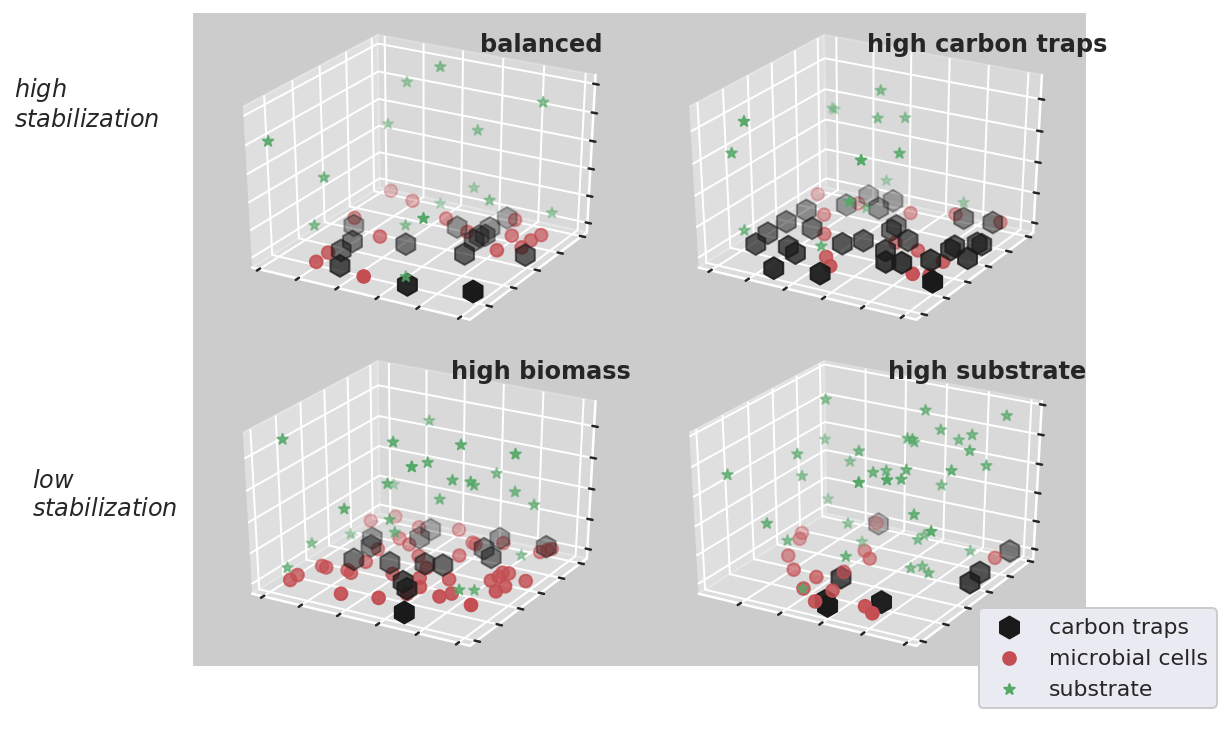
\includegraphics[scale=0.8]{thesis_figures/test/model_scenarios.png}
			\caption{examples of the different model scenarios with their corresponding outcome on the far left side of the figure}
			\label{fig:stabilization_model_scenarios}
		\end{figure}
		
		In the current experiment, a series of three consecutive, high rate applications of highly labile organic substrate was setup, each portion causing a rapid increase in microbial biomass followed by period of diminishing MB. In the first week for example, this strong microbial turnover likely yielded a large quantity of available carbonaceous organic substances in the form of necromass and other microbial products in the days following peak microbial growth
		(‘secondary pulse’),
		% microbial death
		and It is reasonable to assume that a substantial portion of this secondary pulse was still present in some sort of readily available form 7 days after MRE application (‘leftover carbon’), when a subsequent input was applied.
		% 	 \myRed{Substantial increases in net HWES during week 1 and 2 seem to correspond with such 'leftover carbon'}.
		Evidently, in all three LTTs, also the live microbial biomass as well as  aggregate structure had changed considerably between one MRE application and the next, particularly in the first and second weeks of incubation.\\
		Examined in light of the proposed stabilization model, these changes imply a modified setting into which MRE is applied in the 2nd and 3rd week. the large amount of labile carbon applied at $ T_0 $ had caused a surge of microbial growth (model variable (1)) which as suggested above, consequently resulted in a secondary pulse of large quantities of readily available microbial products (model variable (2)) yet proposedly, these pulses were not accompanied by proportional increases in potential sites of OM stabilization(variable (3)). considering the soil system right after the 2nd MRE application it is suggested that the sum of leftover carbon from the first application, along with newly introduced MRE carbon, resulted in a situation corresponding to scenario (1) in the stabilization model,  in which a high substrate-to-biomass ratio but especially high proportion of substrate to available stabilization sites would result in lower \gls{cue}.
		Direct meaningful  assessment of \gls{om} stabilization was not possible using data from the current experiment,
		it is assumed therefore that my \gls{cue} results provide a viable indication of the efficiency of short term \gls{om} stabilization (i.e the fraction of substrate-C remaining in the soil).\\
		%			 microbial products and necromass as primary source of stable \gls{som}
		microbial growth and respiration data in the 1st incubation week, seems to be in full agreement with the above proposed mechanism for reduced \gls{cue}. all three LTTs had seen a considerable increase in the weekly cumulative respiration while simultaneously presenting a notable decrease in the weekly microbial growth. the proportion of weekly respired $ CO_2 $-$ C $ to the weekly MRE-C applied had increased by roughly 10\% between the 1st and 2nd week while this same proportion for weekly microbial growth, decreased by more than tenfold for ORG and UNC and by a little more than half for MIN. given the validty of assumptions \ref{item: complete_uptake} and \ref{item: negligible_priming} of complete uptake and neglible priming, the inefficient use of MRE input in the 2nd, compared with the 1st week becomes evident. \\
		%	 \myRed{how exactly is the efficiency of microbial growth related to the efficiency of carbon stabilization, i.e \%stabilization?}\\
		according to the suggested 'stabilization model', higher substrate-to-biomass and a higher proportion of these two features to the availability of stabilization sites (or 'carbon traps'), would results in a smaller fraction of substrate-C remaining in the soil matrix, not necessarily less MBC being accumulated (as was observed in my results). however, it is suggested here that, besides ensuring carbon stabilization efficiency, a balanced proportion of available substrate, microbial biomass and soil pore availability for carbon protection, will also be reflected in more efficient accumulation of MB which would presumably result in a higher \%stabilization.\\
		%todo why higher biomass accumulation results in higher stabilization
		another soil feature that presented a strong reaction to consecutive MRE additions was the WEOC fraction. large pulses of WEOC were observed after each MRE addition (for the first week mainly in UNC) and these pulses increased considerably ( particularly for UNC and MIN) with consecutive additions. likewise the extent of these pulses was positively correlated with lower respiration rate and lower biomass among the three LTTs. this clearly points out to a phenomena mentioned earlier, whereby reduced microbial activity is reflected in greater accumulation of labile organic carbon, at least in the short term of a couple of days. in the 2nd week these trends in WEOC coincide with greatly reduced \gls{cue} in all three LTTs, and especialy in UNC, which incidently also had the highest WEOC accumaltion 24 h after MRE addition on that week. it seems that, mainly for UNC and MIN, the surge of easily available organic substrate ( from both 'leftover carbon' as well as from newly introduced MRE) has caused the microbial biomass to be overwhelmed, considerably reducing the uptake and utilization rate of available substrate in the first day or two after MRE addition and concurently also resulting in reduced weekly \gls{cue}.
		This was not the case for ORG, as the clear reduction in \gls{cue} was not accompanied by substantial pulses of WEOC.
		
		\section{Short term dynamics of \gls{som} pools in amended soils}
		%todo rephrase above title
		%todo rewrite opening section. shorter recap of the previuos section and include the opening of next subsection
		
		In this work, I’ve attributed particular importance to the proportion of Microbial growth to microbial respiration, expressed as the \gls{cue} index, as it was postulated to reflect to a large degree, the efficiency of incoming \gls{om} stabilization and incorporation into \gls{som}. This approach has proven to be at least partially successful in illustrating the effect of sequential labile substrate applications, as it indicated a reduction in \gls{cue} with each subsequent MRE addition. A much more limited success was achieved in trying to distinguish the effect of management history on the short term dynamics of \gls{som} pools, using  the \gls{cue} index. As noted earlier, ORG and MIN displayed a very similar  reduction in \gls{cue} throughout the incubation, while a somewhat erratic pattern was observed for UNC. Additionally, large uncertainties are associated with the weekly \gls{cue} results making it hard to assert  meaningful distinction between LTTs.\\ \pdfmargincomment[height=40pt]{I meant this opening section to lead to the fact that other parameters (like WEOC and HWES) revealed the effect of management history as opposed to CUE...}
		
		\subsection{Variability in WEOC removal}
		The dynamics of MBC by itself, also did not seem to reveal any significant differences between LTTs in their response to MRE input.
		However, the dynamics of CO2-Resp and moreover those of WEOC, in MRE amended samples, suggest a notable effect of management history on \gls{som} dynamics in this short term incubation. WEOC levels had peaked at almost 1000 mg/kg  24 h after the first MRE addition in UNC samples and the corresponding peak 24 h after the third MRE application in these UNC samples was almost double the size of the first peak. Data is missing for the second peak in UNC samples, yet it is assumed to have followed the trend suggested by the large differences between the first and third WEOC peak. This trend is similarly observed in MIN samples, albeit with a significantly lower intensity. Remarkably, these sharp increases in WEOC 24 h after MRE addition, were not observed in ORG on any sampling event.\\
		The intensity of WEOC pulses after each MRE addition increased both in time ( with consecutive MRE applications) and also between LTTs, in the following order, UNC $ > $ MIN $ > $ ORG. This order of response intensity between the three LTTs, most clearly notable 1 day after MRE additions, seems to be largely opposite to the order of baseline SOC content and baseline MBC between these LTTs, which were as follows, ORG $ > $ MIN $ > $ UNC (differences in MBC between ORG and MIN and between MIN and UNC in SOC, are not significant). This suggest  that higher initial \gls{som} content and/or higher extant microbial biomass may have been related to moderated fluctuations in WEOC following MRE additions and to moderated increases in the intensity of these fluctuations as the incubation preceded. \\
		Results from the preliminary incubation are indicative of the important role of microbial respiration in the removal of WEOC from the soil. Both Str or KWC amended soils as well as non-amended samples from the preliminary incubation presented an inverse trend between WEOC and Resp dynamics. However, no significant difference between ORG and MIN (in Str or KWC amended soils) was observed in terms of the efficiency of WEOC removal. In the MRE incubation, a comparison of WEOC dynamics with those of Resp revealed an opposite trend in the order of LTTs throughout most of the incubation. In this way soil samples in which Resp was high presented low WEOC pulses and vice versa. Although the sample size of different LTTs was quite low (N=3), the relation between microbial activity (Resp) and WEOC removal seems apparent. \\
		%	additionally, cumulative respiration in the three LTTs suggests the connection between elevated microbial activity (i.e respiration) and the quick removal of labile organic carbon.
		
		In the current experiment, an exceptionally high load of labile organics was applied with each MRE addition, roughly an order of magnitude higher than baseline MBC values.  Although labile DOM is usually rapidly consumed by the soil microbial population\myRed{*} it is possible that in situations were a proportionally large amount of labile substrate is rapidly introduced, the microbial population would be unable to process it completely\myRed{*} in the very short term of several hours to a day or two, and thus considerable amounts of substrate could be accumulated as WEOM. This seems to have been the case in the current experiment, where in the first week of incubation both ORG and MIN, presumably possessing a significantly higher reserve of active and potentially active microbial biomass, presented a very low increase in WEOC 24 h after MRE addition . This is suggestive of the metabolic capacity of these soil microbial populations allowing them to rapidly consume and break down the input substrate to the extent that it is unrecoverable as WEOM, either by mineralization of the substrate into CO2, its immobilization as MB or its transformation into metabolic products that would have been bound to the solid soil phase.
		%, rendering it unextractable with water.
		In the subsequent MRE additions, it is assumed that-although MRE input load was unchanged-the conditions with regard to microbial biomass and overall labile \gls{om} availability had been altered significantly, resulting in the increased intensity of WEOC pulses in these subsequent MRE additions (in MIN and UNC). As discussed in a previous section, it is suggested that by the end of the first week of incubation, the levels of labile \gls{om} availability had increased substantially (\textit{leftover carbon}). While MBC also increased  considerably in all three LTTs during the first week, it is proposed that the substrate-to-biomass  ratio had increased considerably between the first and second MRE additions in MIN and UNC, which may have been the primary reason for the observed pulses of WEOC following MRE addition, as the microbial populations in these soil samples were ineffective in removing the large influx of DOM during the first 24 h.
		
		In line with the proposed \textit{stabilization model} as well as the evidence presented earlier regarding the nature of DOM, I propose three  major drivers which controlled the dynamics of WEOC in the days following each MRE addition, each one represented by a measured soil feature:
		\begin{enumerate}
			\item microbial assimilation (MBC)
			\item microbial mineralization (CO2-Resp)
			\item potential for \gls{om} stabilization (AS, expressing the potential availability of the soil mineral phase for interaction with incoming decomposition products).
		\end{enumerate}
		
		
		while  CO2 mineralization can explain some of the variation in WEOC between LTTs, it is clearly not enough to explain all of the variation, as evident when comparing cumulative Resp trends with those of WEOC. The largest difference by far between LTT's in the percent change of cumulative respiration, is observed during the first pulse while subsequent pulses presented a much smaller and relatively minor difference between LTTs in terms of percent change in cumulative respiration.
		Microbial assimilation might have accounted for some of the variation yet no significant differences between LTT's were observed during the incubation.
		It seems therefore, that neither microbial growth (anabolism) nor microbial respiration (catabolism) can fully account for the variation between LTTs. The third driver listed above, namely soil potential for \gls{om} stabilization, remains thus as a possible candidate to account for the primary share of this observed variability. It is noted here that my analysis of soil aggregate stability provides only inferential information regarding the dynamics of soil stabilization potential, both due the low sampling frequency during the incubation as well as the nature of the test itself which provides a general indication of the aggregation status of the soil rather than a more detailed characterization of soil spatial organization. For example, an elaborate description of soil pore architecture including for example, pore size distribution and connectivity, could have been much more effective in examining the relation between stabilization potential and microbial efficiency in general and the short term removal of labile \gls{om} from soil solution in particular. \\
		Despite these limitations, AS is nonetheless presumed to provide valuable indications of a soil stabilization potential. The significantly lower \%WSA in UNC compared with the two other LTTs, throughout the incubation, is in accordance with the higher intensity of WEOC pulses in that LTT, suggesting structural features may have been a significant factor in this regard. However, differences between ORG and MIN did not correspond with the variations between these LTTs in terms of WEOC dynamics.  \\
		
		%\section{conclusions \hiddenTxt{limitations of the experimental setup}and suggestions for further research}
		%
		%		This research examined the effect of long term soil management and particularly fertilization management, on \gls{som} pools and related soil features such as AS. Our analysis of the dynamics as well baseline values of non-amended samples, provided strong evidence for the effect of 5 years of contrasting fertilization schemes on \gls{som} pools. These results indicated a clear distinction between organically and mineraly fertilized soil in both total SOC as well as biological \gls{som} pools. That this distinction was observed in soil samples obtained after a substantial resting period (\textit{no input + fallow}) in the original long-term experiment (GOP) is of particular interest.      , results from our MRE as well as Str and KWC amended samples were far more ambiguous.
		
		%The dynamics of WEOC in MRE amended samples present a definite distinction between LTTs, and this distinction matches clearly, though inversely, the variation between LTTs in baseline MBC and Resp. This \myRed{seemingly} negative correlation between WEOC on the one hand and extant microbial biomass on the other hand, similarly observed in all of the incubations during this research, provides strong evidence of the close association of microbial activity and WEOC. It is highly likely then, that increased microbial biomass and particularly active microbial biomass (as reflected in Resp) in the cultivated LTTs as opposed to UNC, had an essential role in driving this differential response between LTTS. This was corroborated to \gls{som}e extent by Resp dynamics during the MRE incubation itself, though not so much by MBC. The fact that microbial respiration is more strongly indicative of the active share of microbial biomass has been discussed earlier in this work. It is therefore not unlikely that the differential response of microbial biomass in terms of removal of WEOC for example, was not significantly reflected in MBC data.
		
		%preliminary incubation
		%	all treatment combinations presented a significant increase in WEOC on the first sampling event which was shortly after followed by a steep decline. the initial increase in WEOC was likely the result of substrate solubilization by water addition and/or microbial action, producing substantial amounts of WEOC. this easily available carbon pool was rapidly and continuously removed in the following days by microbial consumption, resulting in decreased WEOC. this decrease closely coincides with the time frame of maximum respiration, between 0-48 h, after which respiration rates had mostly leveled off. concurrence of WEOC removal with increased Resp levels, also observed for control samples in the preliminary experiment, effectively illustrates the  notion of WEOC as an immediate and labile source of energy for micro-organisms.
		
		
		The dynamics of HWES had also presented considerable variation between LTTs during the 28 days MRE incubation. The hot water extractable fraction of \gls{som} is often associated with aggregation processes, particularly its carbohydrate portion.  However HWEC and specifically HWES are also regarded as a labile source of energy utilized by the microbial population. In the current work, HWES dynamics during the MRE incubation mostly seemed to accord with the later view. When examining the net HWES accumulation in the course of the incubation, there appears to be a similar relation between HWES accumulation and the metabolic capacity of the soil (represented by MBC and moreover microbial Resp), as described above for WEOC. Although this relation is evidently not as clear as for WEOC, it does become more evident at day 21 and certainly at day 28 wherein the order of HWES content between LTTs is opposite with the general order of MBC and Resp as observed throughout my experiments. Clearly the significantly higher net HWES in UNC at days 14, 21 and 28, compared with both cultivated LTTs, is indicative of the lower metabolic capacity of this soil, as was also observed for WEOC. Here again, it remains unclear whether and in what way, the variation in HWES consumption and removal from DOM fraction is connected with microbial \gls{cue} and the carbon stabilization potential. However it appears that microbial capacity for labile carbon removal from DOM fraction is at least to some extent positively related with \gls{cue}, as evident from the inverse general trend in \gls{cue} as opposed to WEOC and HWES across the incubation period.
		

\bibliographystyle{unsrtnat}
\bibliography{thesis_}

\end{document}
